%% Based on a TeXnicCenter-Template by Tino Weinkauf.
%%%%%%%%%%%%%%%%%%%%%%%%%%%%%%%%%%%%%%%%%%%%%%%%%%%%%%%%%%%%%

%%%%%%%%%%%%%%%%%%%%%%%%%%%%%%%%%%%%%%%%%%%%%%%%%%%%%%%%%%%%%
%% HEADER
%%%%%%%%%%%%%%%%%%%%%%%%%%%%%%%%%%%%%%%%%%%%%%%%%%%%%%%%%%%%%
\documentclass[oneside,11pt,review,usenames,dvipsnames]{report}
% Alternative Options:
%	Paper Size: a4paper / a5paper / b5paper / letterpaper / legalpaper / executivepaper
% Duplex: oneside / twoside
% Base Font Size: 10pt / 11pt / 12pt
\setlength{\parskip}{\baselineskip}

%% Packages
\usepackage[letterpaper, paperwidth=170mm, paperheight=225mm, bottom=20mm, right=20mm]{geometry}
\usepackage{amsmath}
\usepackage{amssymb}
\usepackage{amsthm} %paquete para s\'imbolo matem\'aticos
\usepackage[spanish,es-nodecimaldot]{babel} %francais, polish, spanish, ...
\usepackage[utf8]{inputenc}
\usepackage{enumerate}
\usepackage{fancyhdr} %%Fancy headings
\usepackage[T1]{fontenc}
\usepackage{graphicx}
\usepackage{bm}
%\usepackage{subfig} %%Subfigures inside a figure
%\usepackage{pst-all} %%PSTricks - not useable with pdfLaTeX
\usepackage[pdftex,
            pdfauthor={CARLOS OMAR PARDO GOMEZ},
            pdftitle={UN MODELO BAYESIANO Y NO PARAM\'ETRICO DE REGRESI\'ON SOBRE CUANTILES},
            pdfsubject={TESIS PARA EL T\'ITULO DE LICENCIADO},
            pdfkeywords={BAYESIANO CUANTILES NO-PARAM\'ETRICO MODELO ESTAD\'ISTICA REGRESI\'ON},
            pdfproducer={Latex con hyperref},
            pdfcreator={pdflatex}]{hyperref}
\usepackage[ansinew]{inputenc}
\usepackage{lmodern} %Type1-font for non-english texts and characters
\usepackage{longtable} %%For tables, that exceed one page
\usepackage[round]{natbib}
\usepackage{subfig} %para poner subfiguras
\usepackage[nottoc]{tocbibind}
\usepackage{url}
\usepackage{fixltx2e}
\usepackage{dsfont}
\usepackage{fontawesome}
\usepackage{float}
\usepackage{caption}
\usepackage[spanish,onelanguage,ruled]{algorithm2e}

\usepackage{amsmath}
\usepackage{amssymb}
\usepackage{amsthm}
\usepackage{mathtools}

\makeatletter
\def\thm@space@setup{%
  \thm@preskip=20pt \thm@postskip=20pt
}
\renewcommand{\@algocf@capt@plain}{above}% formerly {bottom}
\renewcommand\fs@ruled{\def\@fs@cfont{\bfseries}\let\@fs@capt\floatc@ruled
  \def\@fs@pre{\hrule height.8pt depth0pt \kern2pt}%
  \def\@fs@post{\kern2pt\hrule\relax}%
  \def\@fs@mid{\kern2pt\hrule\kern\baselineskip}% original: \kern2pt\hrule\kern2pt
  \let\@fs@iftopcapt\iftrue}
\renewcommand{\@algocf@capt@plain}{above}% formerly {bottom}
\makeatother

\newcommand*{\finalnamedelim}{%
   \ifnumgreater{\value{liststop}}{2}{\finalandcomma}{}%
   \addspace\&\space}

\usepackage[bottom]{footmisc} 

%% Espaciado
\usepackage{setspace}
%\singlespacing        %% 1-spacing (default)
\onehalfspacing       %% 1,5-spacing
%\doublespacing        %% 2-spacing
\setlength\parindent{0pt} 

%%% Norma %%%
%\newcommand{\norm}[1]{\left\lVert#1\right\rVert}

%%% Valor absoluto %%%
\usepackage{mathtools}
\DeclarePairedDelimiter\abs{\lvert}{\rvert}%
\DeclarePairedDelimiter\norm{\lVert}{\rVert}%
% Swap the definition of \abs* and \norm*, so that \abs
% and \norm resizes the size of the brackets, and the 
% starred version does not.
\makeatletter
\let\oldabs\abs
\def\abs{\@ifstar{\oldabs}{\oldabs*}}
%
\let\oldnorm\norm
\def\norm{\@ifstar{\oldnorm}{\oldnorm*}}
\makeatother
%%% %%%

%%%% R code %%%%
\usepackage{listingsutf8}
\usepackage[usenames,dvipsnames]{color}   
\lstset{ 
  language=R,                     % the language of the code
  basicstyle=\footnotesize \ttfamily,  % the size of the fonts that are used for the code
  numbers=left,                   % where to put the line-numbers
  numberstyle=\tiny\color{Blue},  % the style that is used for the line-numbers
  stepnumber=1,                   % the step between two line-numbers. If it is 1, each line
                                  % will be numbered
  numbersep=5pt,                  % how far the line-numbers are from the code
  backgroundcolor=\color{white} ,,  % choose the background color. You must add \usepackage{color}
  showspaces=false,               % show spaces adding particular underscores
  showstringspaces=false,         % underline spaces within strings
  showtabs=false,                 % show tabs within strings adding particular underscores
  frame=single,                   % adds a frame around the code
  rulecolor=\color{black},        % if not set, the frame-color may be changed on line-breaks within not-black text (e.g. commens (green here))
  tabsize=2,                      % sets default tabsize to 2 spaces
  captionpos=b,                   % sets the caption-position to bottom
  breaklines=false,                % sets automatic line breaking
  breakatwhitespace=false,        % sets if automatic breaks should only happen at whitespace
  keywordstyle=\ttfamily,
  commentstyle=\color{RoyalBlue},   % comment style
  stringstyle=\color{ForestGreen},      % string literal style
  inputencoding=utf8/latin1
} 

\newtheorem{defin}{Definici\'on}
\newtheorem*{defin*}{Definici\'on}
\newtheorem*{obs*}{Observaci\'on}
\newtheorem*{theorem*}{Teorema}
\newtheorem*{prop*}{Propiedad}

\newenvironment{dedication}
  {\clearpage           % we want a new page          
   \thispagestyle{empty}% no header and footer
   \vspace*{\stretch{1}}% some space at the top
   \itshape             % the text is in italics
   \raggedleft          % flush to the right margin
  }
  {\par % end the paragraph
   \vspace{\stretch{3}} % space at bottom is three times that at the top
   \clearpage           % finish off the page
  }

%%%%%%%%%%%%%%%%%%%%%%%%%%%%%%%%%%%%%%%%%%%%%%%%%%%%%%%%%%%%%
%%  Documento
%%%%%%%%%%%%%%%%%%%%%%%%%%%%%%%%%%%%%%%%%%%%%%%%%%%%%%%%%%%%%
\begin{document}

\pagestyle{empty} %No headings for the first pages.

\title{UN MODELO BAYESIANO Y NO PARAM\'ETRICO DE REGRESI\'ON SOBRE CUANTILES} %Con este nombre se guardar\'a el proyecto en writeLaTex

%%%%%%%%%%%%%%%%%%%%%%%%%%%%%%%%%%%%%%%%%%%%%%%%%%%%%%%%%%%%%
%%    Secciones iniciales
%%%%%%%%%%%%%%%%%%%%%%%%%%%%%%%%%%%%%%%%%%%%%%%%%%%%%%%%%%%%%

% COVER PAGE
\begin{titlepage}
\begin{center}

\large{INSTITUTO TECNOLOGICO AUTONOMO DE MEXICO}\\[2em]
\hline

%Figura
\begin{center}
	
\includegraphics{Figures/Miscellaneous/logo-ITAM.pdf}
\end{center}

\vspace{1em}

{\sc {\bf \large UN MODELO BAYESIANO Y NO PARAMETRICO DE REGRESION SOBRE CUANTILES}}\\[3em]

\textsc{\large TESIS}\\[1em]

\textsc{\normalsize QUE PARA OBTENER EL TITULO DE}\\[1em]

\textsc{\normalsize LICENCIADO EN MATEMATICAS APLICADAS}\\[1em]

\textsc{\normalsize PRESENTA}\\[1em]

\textsc{\Large CARLOS OMAR PARDO GOMEZ}\\[3em]

\end{center}

\vspace*{\fill}
\textsc{CIUDAD DE MEXICO \hspace*{\fill} 2017}

\end{titlepage}
% COVER PAGE
\begin{titlepage}
\begin{center}

\large{INSTITUTO TECNOL\'OGICO AUT\'ONOMO DE M\'EXICO}\\[2em]
\hline

%Figura
\begin{center}
	
\includegraphics{Figures/Miscellaneous/logo-ITAM.pdf}
\end{center}

\vspace{1em}

{\sc {\bf \large UN MODELO BAYESIANO Y NO PARAM\'ETRICO DE REGRESION SOBRE CUANTILES}}\\[3em]

\textsc{\large TESIS}\\[1em]

\textsc{\normalsize QUE PARA OBTENER EL T\'ITULO DE}\\[1em]

\textsc{\normalsize LICENCIADO EN MATEM\'ATICAS APLICADAS}\\[1em]

\textsc{\normalsize PRESENTA}\\[1em]

\textsc{\Large CARLOS OMAR PARDO GOMEZ}\\[3em]

\textsc{\normalsize ASESOR: DR. JUAN CARLOS MART\'INEZ OVANDO}

\end{center}

\vspace*{\fill}
\textsc{CIUDAD DE M\'EXICO \hspace*{\fill} 2018}

\end{titlepage}

\thispagestyle{empty}
\vspace*{\fill}
\begingroup
Con fundamento en los art\'iculos 21 y 27 de la Ley Federal del Derecho de Autor y como titular de los derechos moral y patrimonial de la obra titulada "\textbf{UN MODELO BAYESIANO Y NO PARAM\'ETRICO DE REGRESI\'ON SOBRE CUANTILES}", otorgo de manera gratuita y permanente al Instituto Tecnol\'ogico Aut\'onomo de M\'exico y a la Biblioteca Ra\'ul Baill\'eres Jr., la autorizaci\'on para que fijen la obra en cualquier medio, incluido el electr\'onico, y la divulguen entre sus usuarios, profesores, estudiantes o terceras personas, sin que pueda percibir por tal divulgaci\'on una contraprestaci\'on.

\centering

\hspace{3em}

\textsc{Carlos Omar Pardo G\'omez}

\vspace{4em}

\rule[1em]{20em}{0.5pt} % L\'inea para la fecha

\textsc{Fecha}
 
\vspace{6em}

\rule[1em]{20em}{0.5pt} % L\'inea para la firma

\textsc{Firma}

\endgroup
\vspace*{\fill}
\begin{dedication}        
A Mago.
\end{dedication}
%\clearpage
\setcounter{page}{1}
\chapter*{Agradecimientos}
\markboth{AGRADECIMIENTOS}{AGRADECIMIENTOS} % encabezado 
A Martha, porque gran parte de lo que soy, y lo que sueño ser, se lo debo a tu gu\'ia. A Chevo, por el gran esfuerzo que haces todos los d\'ias por los tuyos. A Jany, por ser mi compañera de aventuras. A Carlos, por tu inigualable ejemplo y sabidur\'ia. A Magally, por darle un sentido \'unico a la palabra \textit{apoyo}. A Janda, Rosy, Marina, Benja, Renata, Benjam\'in, Blanquita, Luis y Rebeca, por conformar a nuestra pequeña, pero unida familia.

Al Dr. Mart\'inez Ovando, por su confianza y asesor\'ia para sacar adelante esta tesis. Al Dr. Nieto, por introducirme al mundo de la estad\'istica. Al Dr. Mendoza, porque gracias a \'el las palabras \textit{regresi\'on} y \textit{Bayesiano} aparecen en este trabajo. Al Dr. Horacio, por mostrarme c\'omo llevar el conocimiento te\'orico al mercado laboral. Y a los cuatro, por el esfuerzo que le dedicaron a la revisi\'on de este documento.

A Farf\'an, Sol, Alexa, Ari, Rodo, Shaq, Norman, Cisneros, y Amor, porque despu\'es de tantos años de amistad, los considero una extensi\'on de mi familia. A Mago, por tu legado de bondad e inteligencia. A tu familia, por el gran ejemplo de fortaleza. 

A Lucy, por los debrayes matem\'aticos y no matem\'aticos. A Lobato, Wille y Josman, por las m\'ultiples facetas que desarrollamos juntos. A Alfredo, Joaquín e Isaac, porque estar rodeado de gente tan inteligente me hizo ser mejor. A Luis y Lalo, por llevar nuestra amistad m\'as all\'a de la escuela. Y a todos con los que compart\'i clases en la carrera de Matem\'aticas Aplicadas.

A Pau Chambon, por aceptarme en todas mis facetas. A Jaime y Rubén, por las risas. A La Bambi, porque me ayudaron a derribar muchos de mis prejuicios. A Fer Langarica y Fer Zepeda, porque estudiar Actuar\'ia me dio excelentes amistades.

A Alain, Cass, y Rafa, por la locura que convertimos en realidad. A Belén, Mariana, Adri, Andrea, Naty y Saus, por permitirme guiarlos. A Brenda, por tu intensidad. A Pato y a Fer Landa, por compartir tan buenas charlas. Y, en general, a todos los miembros de Doxia y SALITAM 2015. 

A Omar Trejo, Luis Garc\'ia, Jorge Alag\'on, Abraham Nieto y Conchita Tapia, por confiar en mi capacidad laboral. A Mois\'es Arizpe, a Mario Guerrero, y, en general, a los equipos de Datata, Kantar, BBVA Bancomer y Datio, por lo que han aportado a mi desarrollo profesional.

A Aar\'on, Fer Rubio y Fer Hern\'andez, por nuestras confidencias. A Vann, por lo que compartimos. A Jess, por siempre sacar mi mejor versi\'on. A Irene y Erick Bustamante, por su confianza. A Luis y Napo, por nuestras interesantes conversaciones. A Mary, por tu risa y tu sonrisa. Y a todos los que han aportado a mi crecimiento personal despu\'es de la universidad. 

Finalmente, al ITAM, por una eduaci\'on de tan alta calidad. A quienes intervinieron para que pudiera disfrutar de las becas Baillères y Mancera. A mis exalumnos, porque disfrut\'e mucho compartir conocimiento. Y a los profesores que aportaron a mi crecimiento, entre los que destaco a Guillermo Grabinsky, Zeferino Parada, Felipe Gonz\'alez, Alberto Tubilla, Marcela Gonz\'alez, Sergio Garc\'ia, Isaac Katz, Valeria Moy y Rosario Sarmiento.
\clearpage
\setcounter{page}{1}
\chapter*{Agradecimientos}
\markboth{AGRADECIMIENTOS}{AGRADECIMIENTOS} % encabezado 
¡Muchas gracias a todos!
\pagestyle{plain}
\chapter*{Prefacio}
\markboth{PREFACIO}{PREFACIO} % encabezado 

%%  Contenido
\addtocontents{toc}{\protect\vspace*{\baselineskip}}

El tema de esta tesis es describir un modelo de regresi\'on sobre cuantiles, debido a diversas bondades que presenta sobre el tradicional an\'alisis de regresi\'on a la media. Adem\'as, a través del paradigma bayesiano permite incorporar conocimiento previo del fen\'omeno y presenta una gran flexibilidad, al contar con componentes no param\'etricos. Asimismo, en este trabajo tambi\'en se abordan los modelos tradicionales de regresi\'on, para entender las desventajas contrarrestadas por el nuevo modelo.

El cap\'itulo 1 describe la importancia de las aproximaciones distintas a la regresi\'on a la media, así como la evoluci\'on hist\'orica de este tipo de modelos. El cap\'itulo 2 introduce al paradigma bayesiano y sus fundamentos generales. El cap\'itulo 3 se centra en los modelos bayesianos tradicionales de regresi\'on, tanto a la media, como sobre cuantiles. El cap\'itulo 4 plantea la especificaci\'on no param\'etrica particular del modelo de esta tesis, separ\'andolo de los tradicionales. El cap\'itulo 5 explica el algoritmo necesario para realizar inferencia y predicci\'on. El cap\'itulo 6 muestra simulaciones y aplicaciones del modelo, as\'i como los resultados obtenidos de evaluarlo en diversos conjuntos de datos. Finalmente, el cap\'itulo 7 hace referencia a las conclusiones de esta tesis, adem\'as de describir el trabajo futuro que se podr\'ia desarrollar.

%%%%%%%%%%%%%%%%%%%%%%%%%%%%%%%%%%%%%%%%%%%%%%%%%%%%%%%%%%%%%
%%    Índice
%%%%%%%%%%%%%%%%%%%%%%%%%%%%%%%%%%%%%%%%%%%%%%%%%%%%%%%%%%%%%

\pagestyle{empty}
\begingroup
\setlength{\parskip}{0pt}
\tableofcontents
\endgroup

%%%%%%%%%%%%%%%%%%%%%%%%%%%%%%%%%%%%%%%%%%%%%%%%%%%%%%%%%%%%%
%%    Capitulos
%%%%%%%%%%%%%%%%%%%%%%%%%%%%%%%%%%%%%%%%%%%%%%%%%%%%%%%%%%%%%

\clearpage
\pagestyle{fancy}
\fancyhf{}
\fancyhead[R]{\nouppercase{\leftmark}}
\cfoot{\thepage}

\chapter{Introducci\'on}

Detr\'as de cualquier modelo de regresi\'on la intenci\'on es entender alguna caracter\'istica asociada con una variable aleatoria, en funci\'on de un conjunto de variables potencialmente explicativas o predictivas para tal caracter\'istica. Ha sido com\'un resumir esta dependencia mediante alguna medida de tendencia central, condicionada a los valores de las covariables.

La medida de tendencia central tradicionalmente usada ha sido la media, dando lugar a los modelos de \textit{regresi\'on a la media}, con sus variantes lineal y no lineal, simple y m\'ultiple, con error normal y no normal. Este tipo de modelos tiene un buen n\'umero de ventajas, entre las que destacan el bajo costo de estimaci\'on y la facilidad de interpretaci\'on de sus par\'ametros (cuando el modelo es param\'etrico). Sin embargo, como mencionan \cite{Hao_FrecQuantReg}, tienen tres grandes limitaciones, que a continuaci\'on se mencionan.

La primera es que, generalmente, la estimaci\'on del modelo busca minimizar la diferencia entre el valor esperado te\'orico y la media observada. Por lo tanto, la inferencia de los valores lejanos a la media, que suelen ser de inter\'es en ciertos contextos, como los seguros o las finanzas, puede ser inexacta.

La segunda es que algunos fen\'omenos de estudio tienen distribuciones de colas pesadas, principalmente en las ciencias sociales. Esto da lugar a valores at\'ipicos, mismos que pueden sesgar estimaciones de la media, mientras prácticamente no afectan a otros estadísticos, como la mediana.

La tercera es que al focalizar la intervenci\'on de las variables explicativas \'unicamente en la media, y darle una distribución predefinida al error, se suelen dejar de lado caracter\'isticas del fen\'omeno que se est\'a estudiando. Un ejemplo es cuando se supone simetr\'ia o asimetr\'ia para todos los errores, pero en los datos se dan ambas condiciones, dependiendo del valor de las variables explicativas. 

Debido a esto, desde mitades del siglo XVIII han surgido alternativas a este tipo de modelos. Seg\'un \cite{Hao_FrecQuantReg}, la primera conocida data de 1760, cuando el jesuita croata Rudjer Josip Boscovich visit\'o Londres en b\'usqueda de consejo computacional para su novedoso modelo de \textit{regresi\’on a la mediana}. De nueva cuenta se busc\'o una medida de tendencia central, pero con otras bondades. Por ejemplo, ser una mejor medida informativa para distribuciones asim\'etricas y menos susceptible a valores at\'ipicos. 

As\'i como los modelos de regresi\'on a la media son com\'unmente relacionados con la minimizaci\'on de los errores cuadr\'aticos, los modelos de regresi\'on a la mediana lo son con la minimizaci\'on de los errores absolutos. Debido a la no diferenciabilidad, tuvieron que pasar muchos años para que lograran ser viables, hasta que el poder computacional y los algoritmos de programaci\'on lineal lo permitieron.

Cabe recordar que, a grandes rasgos y sin dar a\'un una definici\'on formal, el cuantil $p$-\'esimo es aquel valor tal que el $p \times 100\%$ de los valores est\'an por debajo de \'el, y el $(1-p)\times 100\%$, por encima. As\'i, la mediana es un caso particular de un cuantil, espec\'ificamente el $0.5$-\'esimo. Esto abre la idea de que otros cuantiles tambi\'en podr\'ian ser modelados en funci\'on de las covariables y no necesariamente tienen que ser una medida de tendencia central. 

Los \textit{modelos de regresi\'on sobre cuantiles} fueron introducidos por \cite{Koenker_QuantReg}, y han permitido concentrarse en valores de inter\'es para los modeladores, sin importar que est\'en alejados de la media. Adem\'as, el c\'alculo de diversos cuantiles para un mismo fen\'omeno ha permitido entender mejor la forma y propiedades de las distribuciones condicionales de la variable de respuesta.

En el paradigma Bayesiano el desarrollo de este tipo de modelos ha sido posterior al de otros paradigmas, y a\'un hay mucho por explorar. \cite{Walker_BayesAccFail}, \cite{Kottas_BaySemiparamMed} y \cite{Hanson_PolyaTrees} desarrollaron modelos para la mediana, suponiendo una distribuci\'on no param\'etrica del error. \cite{Yu_BayQuantReg} y \cite{Tsionas_BayQuantInf} desarrollaron inferencia param\'etrica, basados en la distribuci\'on asim\'etrica de Laplace para los errores. Por otro lado, \cite{Lavine_LikeQuant} y \cite{Dunson_ApproxBayes} usaron una perspectiva distinta y propusieron una aproximaci\'on de la verosimilitud para cuantiles.

Por la misma naturaleza compleja del nuevo desaf\'io, los modelos de regresi\'on sobre cuantiles han retomado un concepto que tambi\'en ha tomado auge en los de regresi\'on a la media: la distribuci\'on no param\'etrica de los errores, misma que generaliza la idea tradicional del error normal. 

Desafortunadamente, a diferencia de los modelos de regresi\'on a la media, que ya han propuesto alternativas para este tema, los modelos Bayesianos de regresi\'on sobre cuantiles han hecho muy poco por romper con la relaci\'on lineal en los par\'ametros entre la variable de respuesta y las covariables. Aquellos que lo han logrado, han tenido que recurrir a estimaciones no probabil\'isticas o no Bayesianas, para resolver alguna parte del problema.

Esta tesis tiene la finalidad de sustituir simult\'aneamente las ideas tradicionales de regresi\'on a la media, linearidad y distribuci\'on param\'etrica de los errores, con un enfoque m\'as flexible y totalmente probabil\'istico. Para ello, rescata las ideas de \cite{Kottas_NotParamQuantReg} y \cite{Kottas_SemiparamQuantReg}, proponiendo un modelo Bayesiano y no param\'etrico, \'util en el contexto de regresi\'on sobre cuantiles.

\newpage
\chapter[Paradigma bayesiano]{Paradigma bayesiano\footnote{Las ideas de este cap\'itulo son retomadas de \cite{Denison_BayesMethods}.}\textsuperscript{,}\footnote{Esta tesis da como aceptados los axiomas de la Estad\'istica Bayesiana, mismos que pueden ser encontrados, por ejemplo, en \cite{Fishburn_Axioms}. Por lo tanto, entiende a dicho paradigma como el coherente para hacer estad\'istica, cuando una toma de decisi\'on con incertidumbre es el objetivo final del estudio. 
}}

\section{Inferencia de variables aleatorias}

Un problema clásico de la estad\'istica es el de hacer predicci\'on, utilizando la informaci\'on de los datos que ya han sido observados. Por ejemplo, es posible pensar que ya se tiene el conjunto de $n$ datos observados $\{y_1, ..., y_n\}$ y se desea hacer predicci\'on acerca del valor del dato $y_{n+1}$, que a\'un no ha sido observado. Para esto, se podr\'ia usar la probabilidad condicional
\begin{equation*}
    \mathbb{P}(y_{n+1}|y_1,...,y_n) =
    \frac{\mathbb{P}(y_{n+1} \cap \{y_1, ..., y_n\})}{\mathbb{P}(y_1, ..., y_n)} =
    \frac{\mathbb{P}(y_1, ..., y_n,y_{n+1})}{\mathbb{P}(y_1, ..., y_n)},
\end{equation*}
pero esto requerir\'ia conocer la funci\'on conjunta, misma que puede ser compleja por la estructura de dependencia de los datos.\footnote{Cabe resaltar que en este trabajo se usar\'a la notaci\'on $\mathbb{P}$ como una forma general de definir una medida de probabilidad, independientemente de los asociados detalles te\'oricos sobre an\'alisis y medibilidad.}

Este problema puede ser abordado mediante el Teorema de representaci\'on general de de Finetti. Para ello, antes se dar\'a una definici\'on.

\begin{defin*}
    Sea $(y_1,...,y_n)$, una secuencia de $n$ variables aleatorias, cuya distribuci\'on de probabilidad conjunta est\'a dada por $\mathbb{P}(y_1,...,y_n)$. Sea $\psi$ una funci\'on biyectiva, que va de $\{1,...,n\} \rightarrow \{1,...,n\}$, es decir, una funci\'on que crea una permutaci\'on del conjunto $\{1,...,n\}$.  
    Entonces, se dice que $(y_1,...,y_n)$ es una \textbf{secuencia aleatoria infinitamente intercambiable} si se cumple que 
    \begin{equation*}
        \mathbb{P}(y_1,...,y_n) = \mathbb{P}(y_{\psi(1)},...,y_{\psi(n)}),
    \end{equation*}
    para cualquier permutaci\'on $\psi$.
\end{defin*}

En pocas palabras, una secuencia $(y_1,...,y_n)$ se considerar\'a infinitamente intercambiable si el orden en que se etiquetan las variables no afecta su distribuci\'on conjunta. Es importante hacer notar que la com\'unmente usada independencia implica intercambiabilidad, pero lo contrario no se cumple. Es decir, la intercambiabilidad es un supuesto menos r\'igido que la independencia.

Dicho esto, es momento de plantear el \textbf{\textit{Teorema de represesentaci\'on general de de Finetti}}.\footnote{Una demostraci\'on de este teorema puede ser encontrada en \cite{Schervish_TheoryStats}.}

\begin{theorem*}
    Sea $(y_1, ...,y_n)$ una secuencia aleatoria infinitamente intercambiable de valores reales. Entonces existe una distribuci\'on de probabilidad $F$ sobre $\mathcal{F}$, el espacio de todas las distribuciones, de forma que la probabilidad conjunta de $(y_1, ...,y_n)$ se puede expresar como
    \begin{equation*}
        \mathbb{P}(y_1, ...,y_n) =
        \int_{\mathcal{F}}\left[\prod_{k=1}^n \mathbb{P}(y_k|G)\right]dF(G),
    \end{equation*}
    con
    \begin{equation*}
        F(G) = \lim_{n \to \infty} F(G_n),
    \end{equation*}
    donde $F(G_n)$ es una funci\'on de distribuci\'on evaluada en la funci\'on de distribuci\'on emp\'irica definida por
    \begin{equation*}
        G_n(y) = \frac{1}{n} \sum_{i=1}^n I(y_i \leq y).
    \end{equation*}
    En otras palabras, el Teorema de de Finetti dice que $\{y_1, ...,y_n\}$ es un conjunto de variables aleatorias condicionalmente independientes, dada cierta distribuci\'on $G$. A su vez dicha $G$ es aleatoria y sigue una distribuci\'on $F(G)$.
\end{theorem*}

Cabe hacer notar que dicho teorema plantea la distribuci\'on conjunta de $(y_1, ...,y_n)$ como una mezcla de verosimilitudes condicionalmente independientes en $G$, donde el peso asociada a cada una depende de $F(G)$. Por lo tanto, $F(G)$ expresa la creencia o conocimiento acerca de cu\'an probable es que $G$ sea id\'oneo para explicar el fen\'omeno, a\'un sin observar los datos.

Un subconjunto del espacio de todas las distribuciones $\mathcal{F}$ es el espacio de las distribuciones param\'etricas, es decir, aquellas que pueden ser descritas en su totalidad \'unicamente señalando el valor de un vector de par\'ametros de tamaño finito $\theta$, mismo que puede tomar valores en todo el soporte $\Theta$. Por lo tanto, si se hace el supuesto adicional que la distribuci\'on marginal de $y_i$ es param\'etrica, con vector de par\'ametros desconocido, se obtiene como corolario del Teorema de de Finetti que
\begin{equation*}
    \mathbb{P}(y_1, ...,y_n) =
    \int_{\Theta}\left[\prod_{k=1}^n \mathbb{P}(y_k|\theta)\right]\mathbb{P}(\theta)d\theta.
\end{equation*}

Siguiendo el razonamiento anterior, $\mathbb{P}(\theta)$ indica la probabilidad de que $\theta$ sea el vector de par\'ametros id\'oneo para explicar el fen\'omeno, antes de observar cualquier dato.

La intuci\'on detr\'as de este resultado es que, al igual que en otros paradigmas, se supone a $\theta$ como constante, pero desconocido, y la tarea es estimarlo. Una particularidad del paradigma bayesiano es expresar la incertidumbre que tiene el modelador acerca del valor verdadero mediante la asignaci\'on de una distribuci\'on a $\theta$, sujeta la informaci\'on inicial o conocimiento previo que se tenga del fen\'omeno $(H)$. Es decir, $\mathbb{P}(\theta|H)$. Como una simplificaci\'on de la notaci\'on, en la literatura normalmente se escribe como $\mathbb{P}(\theta) = \mathbb{P}(\theta|H)$ y se conoce como la \textit{probabilidad inicial} del par\'ametro.

Regresando al problema inicial, y bajo los supuestos reci\'en mencionados, es posible escribir
\begin{equation*}
    \mathbb{P}(y_{n+1} | y_1,...,y_n) =
    \int_{\Theta} 
    \mathbb{P}(y_{n+1}|\theta) \mathbb{P}(\theta|y_1,...y_n)d\theta,
\end{equation*}
donde a su vez, usando el \textbf{Teorema de Bayes}, se obtiene que
\begin{equation*}
\begin{aligned}
    \mathbb{P}(\theta|y_1,...,y_n) &=
    \frac{\mathbb{P}(y_1,...,y_n|\theta)\times\mathbb{P}(\theta)}
    {\mathbb{P}(y_1,...,y_n)},
\end{aligned}
\end{equation*}
que en el paradigma bayesiano se conoce como la \textit{probabilidad posterior} del par\'ametro. 

Se puede observar que el denominador no depende de $\theta$, y en realidad es una constante dada por la representaci\'on del teorema de de Finetti de la probabilidad conjunta, por lo que normalmente la probabilidad condicional del vector de par\'ametros no se expresa como una igualdad, sino con la proporcionalidad
\begin{equation*}
    \mathbb{P}(\theta|y_1,...,y_n) 
    \propto 
    \mathbb{P}(y_1,...y_n|\theta) \times \mathbb{P}(\theta),
\end{equation*}
y s\'olo difiere de la igualdad por una constante que permita que, al integrar sobre todo el soporte de $\theta$, el resultado sea igual a 1.

Cabe resaltar que el factor $\mathbb{P}(y_1,...y_n|\theta)$ es lo que se conoce tambi\'en en otros paradigmas como \textit{verosimilitud}, y que en caso de independencia condicional puede ser reescrito como
\begin{equation*}
    \mathbb{P}(y_1,...,y_n|\theta)  = \prod_{i=1}^n \mathbb{P}(y_i|\theta).
\end{equation*}
Por lo tanto, es posible afirmar que el aprendizaje en el paradigma bayesiano se obtiene como
\begin{equation*}
    Posterior \propto Verosimilitud \times Inicial,
\end{equation*}
es decir, surge de conjuntar el conocimiento inicial con la informaci\'on contenida en los datos.

Es importante notar que bajo este enfoque se obtiene una distribuci\'on de probabilidad completa para  el pron\'ostico de $y_{n+1}$. \'Esta se puede utilizar para el c\'alculo de estimaciones puntuales o intervalos (que en el caso del paradigma bayesiano son llamados de \textit{probabilidad}) mediante funciones de utilidad o p\'erdida, y haciendo uso de la Teor\'ia de la Decisi\'on.

\section{Propiedad conjugada}

En los casos en los que la probabilidad posterior, que resulta del producto de la verosimilitud y la inicial, pertenece a la misma familia de la distribuci\'on inicial, \'unicamente difiriendo en el valor de los par\'ametros, se dice que la distribuci\'on de los par\'ametros y la verosimilitud pertenecen a una \textbf{familia conjugada}.

Esta propiedad es conveniente, porque permite a la distribuci\'on posterior tener forma anal\'itica cerrada, evitando tener que usar m\'etodos num\'ericos para aproximarla. Adem\'as permite ver de forma m\'as clara c\'omo afectan los datos a la actualizaci\'on, respecto a la distribuci\'on inicial.

Algunas de las familias conjugadas m\'as conocidas son la \textit{Normal-Normal}, \textit{Normal-Gamma}, \textit{Normal-Gamma Inversa}, \textit{Bernoulli-Beta} o la \textit{Poisson-Gamma}, donde la primer distribuci\'on representa a la verosimilitud y la segunda, la distribuci\'on de los par\'ametros. 

Sin embargo, el rango de posibles modelos conjugados puede resultar limitado en algunos contextos pr\'acticos debido a que el fen\'omeno en estudio puede ser mejor representado con ciertas distribuciones espec\'ificas, que usualmente no pertenecen a familias conjugadas.

\section[Inferencia con variables predictivas]{Inferencia con variables predictivas\raisebox{.3\baselineskip}{\normalsize\footnotemark}}\footnotetext{Esta secci\'on carece de formalidad, pero busca darle la intuici\'on al lector para generalizar el resultado del teorema de de Finetti en el contexto en el que se desarrollar\'a este trabajo. Para una explicaci\'on formal, consultar \cite{Dawid_Exchangeability}.}

Como se ver\'a en el siguiente cap\'itulo de esta tesis, un problema com\'un es estimar la distribuci\'on de cierta secuencia de variables aleatorias $(y_1,...,y_n)$, condicionadas a los valores $(x_1,...,x_n)$ de otras variables com\'unmente llamadas predictivas. En este caso, la secuencia $(y_1,...,y_n)$ ya no es intercambiable, porque cada valor $y_i$ depende en alguna medida del valor de su respectiva $x_i$, por lo que no es posible aplicar de manera directa el teorema de de Finetti. Para hacerlo de manera indirecta, se introducir\'a el t\'ermino de intercambiabilidad parcial.

\begin{defin*}
    Sea $(y_1|x_1,...,y_n|x_n)$, una secuencia de $n$ variables aleatorias, condicionales en los valores de ciertas variables predictivas, cuya distribuci\'on de probabilidad conjunta est\'a dada por $\mathbb{
    P}(y_1,...,y_n|x_1,...,x_n)$. Sea $\psi$ una funci\'on biyectiva, que va de $\{k_1,...,k_r\} \rightarrow \{k_1,...,k_r\}$, es decir, una funci\'on que crea una permutaci\'on del conjunto $\{k_1,...,k_r\}$; y $\tilde{x}_1,..., \tilde{x}_1$ los distintos valores \'unicos que toman las $x_i's$.  
    Entonces, se dice que $(y_1,...,y_n)$ es una \textbf{secuencia aleatoria infinita y parcialmente intercambiable} si se cumple que 
    \begin{equation*}
        \mathbb{P}(y_{k_1},...,y_{k_r}|\tilde{x}_k) = \mathbb{P}(y_{\psi(k_1)},...,y_{\psi(k_r)}|\tilde{x}_k),
    \end{equation*}
    para cualquier permutaci\'on $\psi$ y para todos los diferentes valores $k$.
    
    Es decir, todas aquellas $y_i's$ cuyas $x_i's$ tienen el mismo valor, son infinitamente intercambiables entre s\'i. 
\end{defin*}

Si adem\'as se cumpliera que el orden de los valores \'unicos $\tilde{x}_k's$ es intercambiable, entonces, intuitivamente se podr\'ia tomar la $G$ del teorema de de Finetti como dependiente de las $x_i$'s, $G(x_i)$, y se obtendr\'ia que
\begin{equation*}
    \mathbb{P}(y_1, ...,y_n|x_1,...,x_n) =
    \int_{\mathcal{F}}\left[\prod_{k=1}^n \mathbb{P}(y_k|G(x_i))\right]dF(G(x_1,...,x_n)),
\end{equation*}
donde las $y_i$'s resultar\'ian ser independientes entre s\'i, condicionadas a una distribuci\'on que depende la $x_i$ asociada.

El tema del siguiente cap\'itulo ser\'a la discusi\'on de m\'etodos de inferencia sobre las variables $y$, dentro de este contexto espec\'ifico de dependencia de una variable predictiva $x$, normalmente conocidos como \textbf{modelos de regresi\'on}.

\newpage
\chapter[Modelos de regresi\'on]{Modelos de regresi\'on}

\section{Concepto de regresi\'on}

Los modelos de regresi\'on tienen como objetivo describir la distribuci\'on de una variable aleatoria $y \in \mathbb{R}$, generalmente llamada \textit{variable de respuesta}, condicional a los valores de las variables $x \in \mathbb{R}^n$, conocidas como \textit{covariables}, \textit{variables explicativas} o \textit{variables predictivas}. Visto en t\'erminos matem\'aticos, se puede expresar como
\begin{equation*}
    y|x \sim \mathbb{P}(y|x).
\end{equation*}

Si bien esta relaci\'on se da por hecha y se supone un v\'inculo concreto del que provinieron los datos, normalmente dicho v\'inculo es desconocido. Por lo tanto, la intenci\'on de estos modelos es realizar alguna estimaci\'on de \'el. Dado que es complicado aproximar con exactitud toda la distribuci\'on, com\'unmente se utilizan un n\'umero finito de par\'ametros para describirla. Adem\'as, la interpretaci\'on de dichos par\'ametros suele tener relevancia para el modelador, como es el caso de la media o la mediana. 

Tambi\'en es importante resaltar que este trabajo tiene inter\'es en modelar a $y$, dado que ya se observaron los valores de $x$. Sin embargo, se podr\'ia pensar en modelos donde tenga sentido la distribuci\'on conjunta de $y$ y $x$, misma que se podr\'ia obtener como
\begin{equation*}
    \mathbb{P}(y,x) = \mathbb{P}(y|x) \times \mathbb{P}(x).
\end{equation*}

\section{Regresión a la media}

\subsection{Planteamiento general}

La \textit{regresi\'on a la media} es el caso m\'as usado dentro de los modelos de regresi\'on, tanto en el paradigma Bayesiano, como en otros. Esto sucede debido al bajo uso de recursos que requiere su estimaci\'on. En el caso particular Bayesiano, diversas familias conjugadas tienen sentido dentro de este contexto; y en otros paradigmas, tambi\'en suelen ser utilizados debido a que se asocian con la minimizaci\'on de t\'erminos cuadrados, con las bondades de diferenciabilidad que eso implica. 

En notaci\'on probabil\'istica, retomando el hecho de que $y|x \sim \mathbb{P}(y|x)$, el modelo de regresi\'on a la media busca aproximar a la funci\'on $f$, tal que 
\begin{equation*}
    f(x) = \mathbb{E}[y|x].
\end{equation*}
Para hacer esto, normalmente se vale del supuesto que
\begin{equation*}
    y = f(x) + \varepsilon,
\end{equation*}
con $\varepsilon \in \mathbb{R}$ (denominado com\'unmente como el \textit{error aleatorio}), una variable aleatoria independiente de $x$, tal que $\mathbb{E}[\varepsilon] = 0$. Adem\'as, $f: \mathbb{R}^n \rightarrow \mathbb{R}$ es desconocida, pero fija. As\'i, debido a que la esperanza de la suma es la suma de las esperanzas, se cumple que $\mathbb{E}[y|x] = f(x)$.

Adem\'as, se supone independencia entre los errores. Por lo tanto, sean $\tilde{x}$ las covariables asociadas a la variable de respuesta $\tilde{y}$, y $\dot{x}$ las asociadas a $\dot{y}$, se tiene que $\tilde{y} | \tilde{x}, f$ es condicionalmente independiente a $\dot{y} | \dot{x}, f$.

\subsection[Modelo tradicional]{
    Modelo tradicional
    \footnote{Algunas ideas de esta subsecci\'on son retomadas de \cite{Denison_BayesMethods} y \cite{Bannerjee_BayLinMod}.}
} \label{trad_mean_reg}

La \textit{regresi\'on lineal a la media} es el caso particular m\'as usado en el contexto de regresi\'on a la media. Consiste en definir
\begin{equation*}
    f(x) = x^T\beta,
\end{equation*}
donde $\beta \in \mathbb{R}^n$ se piensa con valores constantes, pero desconocidos, y la tarea es estimarlos. Adem\'as, se supone error normal, es decir, $\varepsilon \sim \mathcal{N}(0,\sigma^2)$, tal que el par\'ametro de varianza fijo $\sigma^2$ tambi\'en debe ser estimado.

Cabe señalar que una gran ventaja de plantear de esta manera el modelo, y por la que ha sido ampliamente usado, es la interpretaci\'on que se le puede dar al vector de par\'ametros $\beta$, como cu\'anto aumenta o disminuye el valor de la variable de respuesta, cuando se aumenta o disminuye una unidad de la variable explicativa.

Sea $\{(x_i,y_i)| x_i \in \mathbb{R}^n, y_i \in \mathbb{R}, i \in \{1,...,m\} \}$ el conjunto de datos observados de las variables de respuesta y de las covariables. Es posible representar este mismo conjunto con la notaci\'on matricial $\{X,Y | X \in \mathbb{R}^{m \times n}, Y \in \mathbb{R}^m\}$. \footnote{Por simplificaci\'on y limpieza de notaci\'on en este trabajo se escribir\'an de igual manera variables aleatorias y los datos en efecto observados, considerando que en cada caso el contexto ser\'a suficiente para saber de cu\'al se est\'a hablando. Por otro lado, se asociar\'an las letras min\'usculas a una \'unica observaci\'on y las may\'usculas a una matriz de observaciones.} Sea $\mathcal{E} \in \mathbb{R}^m$ el vector de errores aleatorios, tal que $\mathcal{E} \sim \mathcal{N}(0,\sigma^2 I)$. El modelo se puede reescribir como
\begin{equation*}
\begin{aligned}
    Y &= X\beta + \mathcal{E} \\
    \implies Y|X,\beta,\sigma^2 &\sim \mathcal{N}(X\beta,\sigma^2 I).
\end{aligned}
\end{equation*}

De esta manera, se tiene una distribuci\'on para el vector aleatorio $Y$, dada la matriz $X$, que para poder ser expresada, requiere de la estimaci\'on de $\beta$ y $\sigma^2$. Para hacer esto, el enfoque Bayesiano le asigna una distribución inicial de probabilidad a ambos par\'ametros, reflejando la incertidumbre que tiene el modelador acerca de su valor real. Es decir, se tiene que 
\begin{equation*}
    \beta,\sigma^2 \sim \mathbb{P}(\beta,\sigma^2).
\end{equation*}

Por el Teorema de Bayes,
\begin{equation*}
\begin{aligned}
    \mathbb{P}(\beta,\sigma^2 | Y, X) 
    &= \frac{\mathbb{P}(Y| X, \beta, \sigma^2) \times \mathbb{P}(\beta, \sigma^2 | X)}{P(Y | X)} \\
    &= \frac{\mathbb{P}(Y| X, \beta, \sigma^2) \times \mathbb{P}(\beta, \sigma^2)}{\mathbb{P}(Y | X)} \\
    &\propto \mathbb{P}(Y| X, \beta, \sigma^2) \times \mathbb{P}(\beta, \sigma^2), \\
\end{aligned}
\end{equation*}
donde $\mathbb{P}(Y| X, \beta, \sigma^2)$ es la verosimilitud de los datos observados, es decir, $ \mathcal{N}(X\beta,\sigma^2 I) = \prod_{i=1}^m \mathcal{N}(x_i^T\beta,\sigma^2)$. 

Por conveniencia anal\'itica, hay una distribuci\'on inicial com\'unmente usada para los par\'ametros $\beta$ y $\sigma^2$ debido a que es conjugada respecto a la distribuci\'on normal de los datos. Su nombre es \textit{Normal-Gamma Inversa (NGI)} y se dice que $\beta,\sigma^2 \sim \mathcal{NGI}(M,V,a,b)$, si
\begin{equation*}
\begin{aligned}
    \mathbb{P}(\beta,\sigma^2) 
    &= \mathbb{P}(\beta|\sigma^2) \times \mathbb{P}(\sigma^2) \\
    &= \mathcal{N}(\beta|M, \sigma^2 V) \times \mathcal{GI}(\sigma ^2|a,b) \\
    &\propto (\sigma^2)^{-(a+(n/2)+1)} \exp\left(-\frac{(\beta-M)^TV^{-1}(\beta-M) + 2b}{2\sigma^2}\right),
\end{aligned}
\end{equation*}
donde $M$ es la media inicial de los coeficientes, $\sigma^2 V$ la matriz de varianzas y covarianzas, y $a$, $b$ son los par\'ametros iniciales de forma y escala, respectivamente, de $\sigma ^2$. 

Aprovechando la propiedad conjugada, es posible escribir la densidad posterior de los par\'ametros como
\begin{equation*}
\begin{aligned}
    \mathbb{P}(\beta,\sigma^2 | Y, X) 
    &\propto \mathbb{P}(Y| X, \beta, \sigma^2) \times \mathbb{P}(\beta, \sigma^2), \\
    &\propto (\sigma^2)^{-(\bar{a}+(n/2)+1)} \exp\left(-\frac{(\beta-\bar{M})^T\bar{V}^{-1}(\beta-\bar{M}) + 2\bar{b}}{2\sigma^2}\right),
\end{aligned}
\end{equation*}
donde
\begin{equation*}
\begin{aligned}
    \bar{M} &= (V^{-1} + X^TX)^{-1} (V^{-1}M + X^TY), \\
    \bar{V} &= (V^{-1} + X^TX)^{-1}, \\
    \bar{a} &= a + m/2, \\
    \bar{b} &= b + \frac{\bar{M}^TV^{-1}M + Y^TY - \bar{M}^T\bar{V}^{-1}\bar{M}}{2}.
\end{aligned}
\end{equation*}

Es decir, la distribuci\'on posterior de $(\beta,\sigma^2)$ es \textit{Normal - Gamma Inversa}, con par\'ametros $\mathcal{NGI}(\bar{M},\bar{V},\bar{a},\bar{b})$.

\section{Regresión sobre cuantiles}

\subsection{Planteamiento general}

Cuando surgi\'o entre la comunidad estad\'istica el problema de regresi\'on sobre cuantiles, inicialmente fue modelado bajo un enfoque no Bayesiano, como se describe en \cite{Yu_BayQuantReg}.  Posteriormente, Koenker \& Bassett (1978) retomaron esas ideas, y las aplicaron en el paradigma Bayesiano. 

La \textit{regresi\'on sobre cuantiles} es una alternativa que se ha desarrollado reci\'entemente y que permite enfocarse en aspectos alternativos de la distribuci\'on, por ejemplo, centrar la estimaci\'on en estad\'isticos que son valores extremos, o en alg\'un decil de inter\'es. 

\begin{defin}
Sea $F_y$ la funci\'on de distribuci\'on acumulada de la variable aleatoria $y$, entonces la funci\'on que regresa su cuantil p-\'esimo se escribe
\begin{equation*}
    q_p(y)\,=\,\inf \left\{x\in {\mathbb  {R}}:p\leq F_y(x)\right\};
\end{equation*}
que se puede simplificar a
\begin{equation*}
    q_p(y)=F_y^{-1}(p),
\end{equation*}
cuando $F_y$ es continua y estrictamente creciente en el soporte de $y$.
\end{defin}
Dicho de manera m\'as intuitiva, si se tiene un conjunto grande de realizaciones de una variable aleatoria $y$, se esperar\'a que el $p \times 100\%$ est\'e por debajo de $q_p(y)$ y el $(1-p) \times 100\%$ est\'e por arriba. Por ejemplo, la mediana es un caso particular de un cuantil, espec\'ificamente el $0.5$-\'esimo. 

Sea el \textit{p-\'esimo} cuantil aquel predefinido como el de inter\'es para el modelador. En notaci\'on probabil\'istica, se buscar\'a aproximar a la funci\'on $f_p$, tal que 
\begin{equation*}
    f_p(x) = q_p(y|x),
\end{equation*}
para $p \in (0,1)$ arbitrario y fijo.

Para hacer esto, normalmente se valdr\'a del supuesto que
\begin{equation*}
    y = f_p(x) + \varepsilon_p,
\end{equation*}
con $\varepsilon_p \in \mathbb{R}$, una variable aleatoria tal que $q_p(\varepsilon_p) = 0$. Asimismo, $f_p: \mathbb{R}^n \rightarrow \mathbb{R}$ es desconocida, pero fija. Por ello, debido a que el cuantil de una suma es la suma de los cuantiles, se cumple que $q_p(y|x) = f_p(x)$.

Al igual que con la regresi\'on a la media, se supone independencia entre los errores, y, por lo tanto, hay independencia condicional entre las observaciones.

\subsection{Modelo tradicional}

Al igual que en la regresi\'on a la media, el primer y m\'as popular modelo ha sido el lineal. Es decir, para $p \in (0,1)$ fijo y elegido por el modelador, se define
\begin{equation*}
    f_p(x) = x^T\beta_p, 
\end{equation*}
donde $\beta_p$ es el vector de coeficientes, dependiente de $p$.

\begin{defin}
    Se define a la funci\'on
    \begin{equation*}
    \begin{aligned}
        \rho_p(u) = u \times [pI_{(u>0)} - (1-p) I_{(u<0)})]
        =
        \begin{cases}
            up &\text{ si } u\geq0 \\
            -u(1-p) &\text{ si } u<0 \\
        \end{cases}
        .
    \end{aligned}
    \end{equation*}

    Se dice que una variable aleatoria u sigue una distribuci\'on asim\'etrica de Laplace ($u|p,\sigma \sim AL_p(\sigma)$) si su funci\'on de densidad se escribe como
    \begin{equation*}
        w_p^{AL}(u|\sigma) = 
        \frac{p(1-p)}{\sigma}
        exp\left[
        -\rho_p
        \left(
        \frac{u}{\sigma}
        \right)
        \right],
    \end{equation*}
con $p$ par\'ametro de asimetr\'ia y $\sigma$, de escala.
\end{defin}

Para entender mejor las propiedades de dicha distribuci\'on, se presentan las siguientes gr\'aficas.
\begin{figure}[H]
	\centering
	\caption{Funci\'on de densidad de la distribuci\'on asim\'etrica de Laplace, con $\sigma = 1$ y $p$ variable.}
	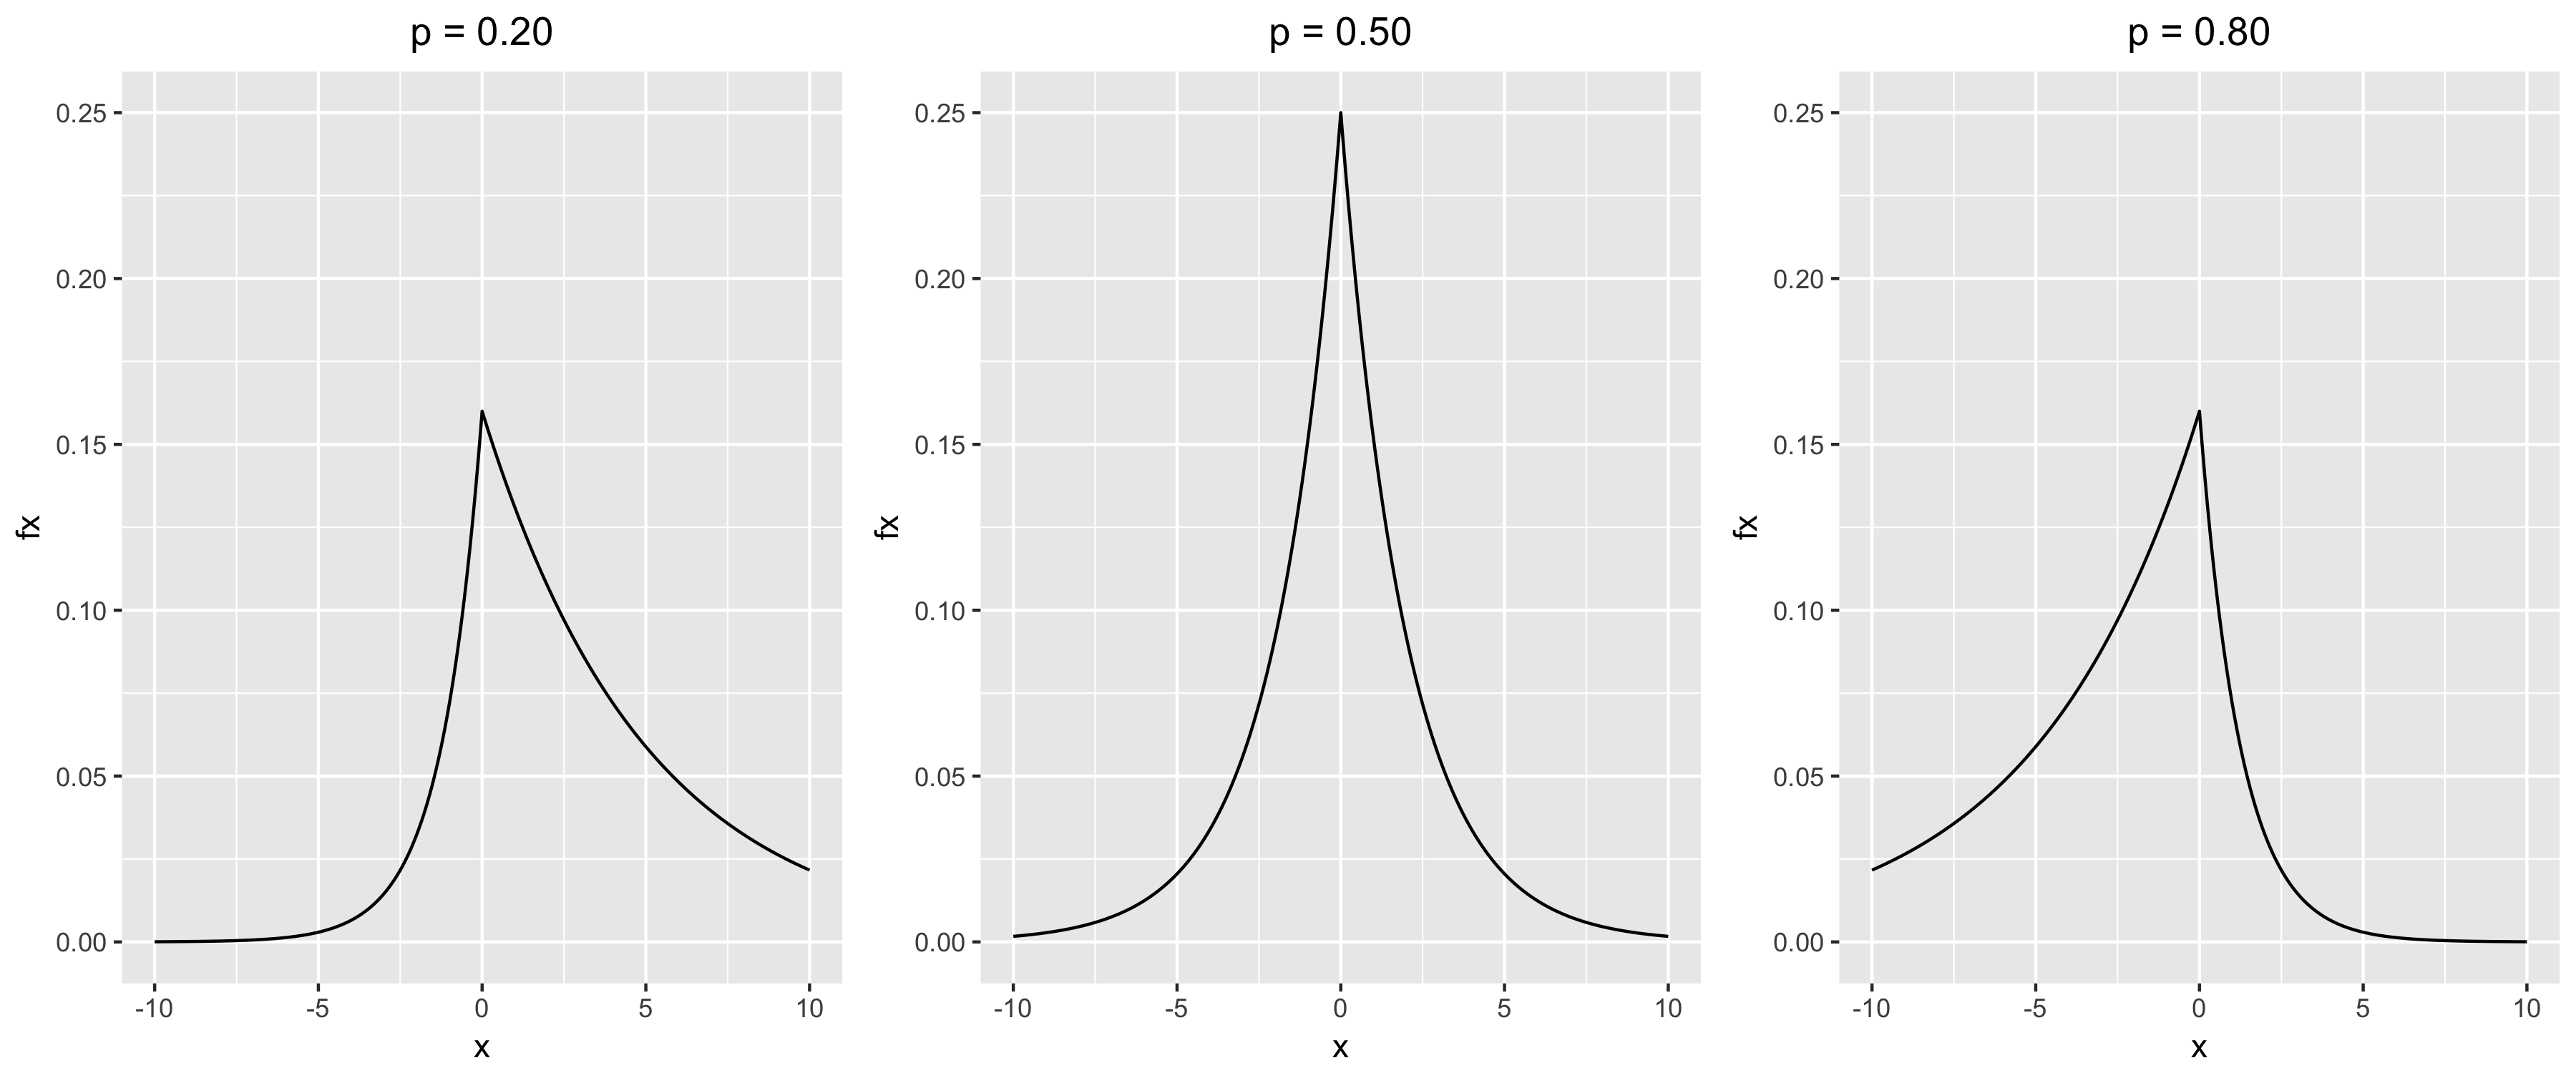
\includegraphics[width=1\textwidth]{Figures/ALD/p_plots.png}
	\label{p_plots}
\end{figure}

\begin{figure}[H]
	\centering
	\caption{Funci\'on de densidad de la distribuci\'on asim\'etrica de Laplace, con $p = 0.25$ y $\sigma$ variable.}
	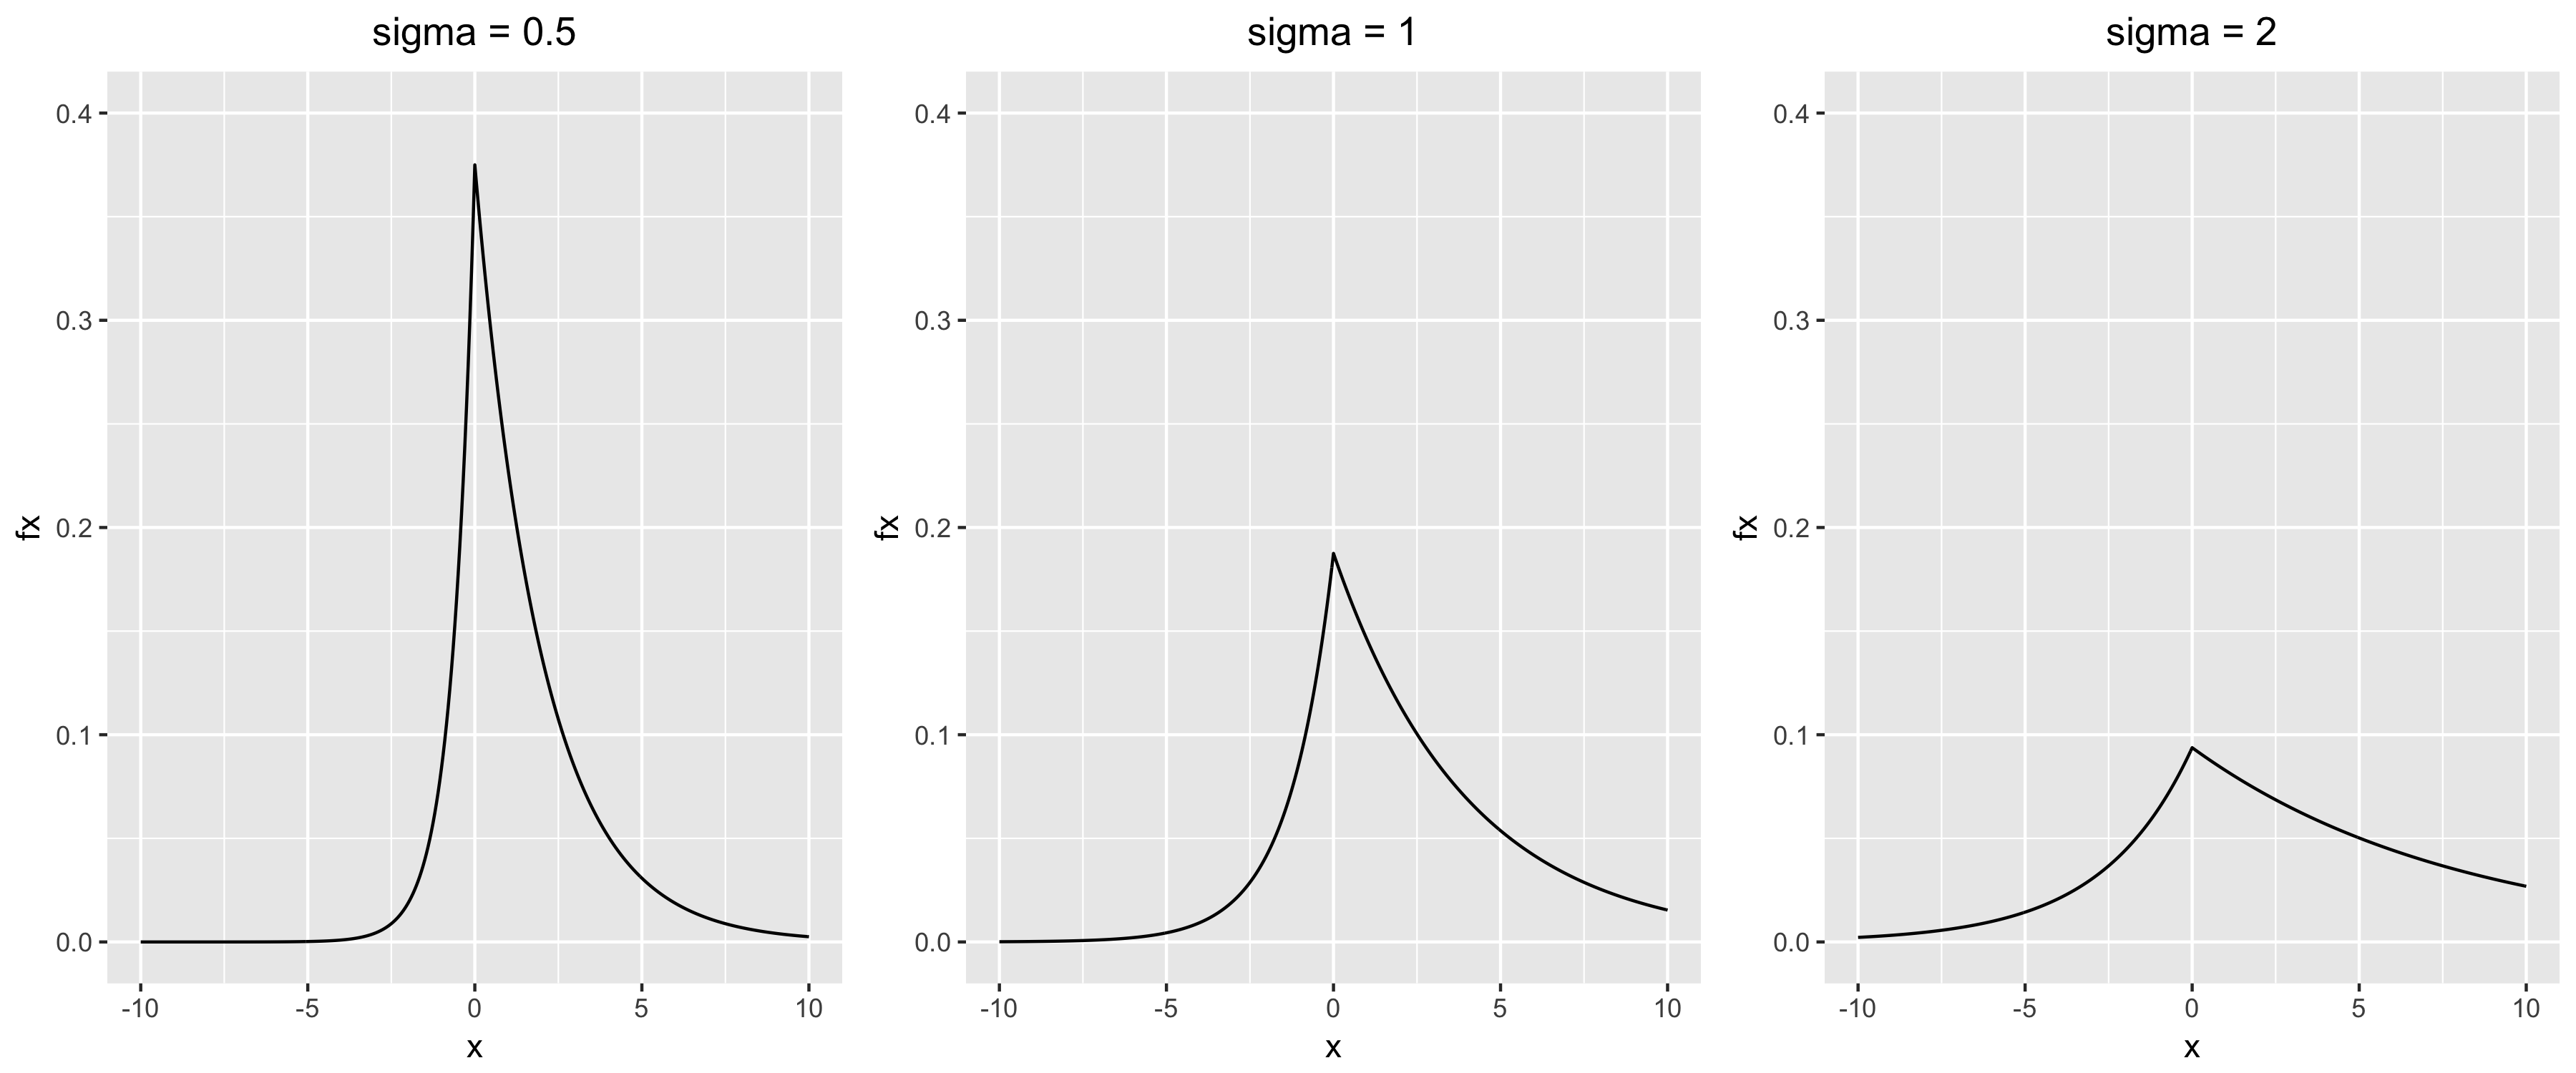
\includegraphics[width=1\textwidth]{Figures/ALD/sigma_plots.png}
	\label{p_plots}
\end{figure}

Como se puede observar, el par\'ametro $p$ representa la asimetr\'ia de la distribuci\'on. Para valores por debajo de $0.5$, la distribuci\'on est\'a sesgada a la derecha, mientras que para valores superiores a $0.5$, presenta sesgo a la izquierda. El \'unico caso en el que es sim\'etrica, es cuando $p = 0.5$. 

Por otro lado, el par\'ametro $\sigma$ representa la dispersi\'on de la distribuci\'on. A menor $\sigma$, los datos, aunque sesgados, estar\'an m\'as concentrados; en cambio, conforme crezca $\sigma$, la cola de la distribuci\'on ser\'a m\'as pesada.

Dicho esto, la propiedad m\'as relevante para este trabajo es que si $\varepsilon_p|\sigma \sim AL_p(\sigma)$, entonces $q_p(\varepsilon_p|\sigma) = 0$, independientemente del valor de $\sigma$. Recordando que esa es la \'unica caracter\'istica que pide el modelo general, el modelo tradicional utiliza esta distribuci\'on para explicar la dispersi\'on del error.

Es posible, entonces, reescribir el modelo como
\begin{equation*}
    y | x, \beta_p, \sigma 
    \sim 
    AL_p(y - x^T\beta_p|\sigma).
\end{equation*}

Sea $\{X,Y | X \in \mathbb{R}^{m \times n}, Y \in \mathbb{R}^m\}$ el conjunto de datos observados. Por el Teorema de Bayes,
\begin{equation*}
\begin{aligned}
    \mathbb{P}(\beta_p,\sigma | Y, X) 
    &\propto \mathbb{P}(Y| X, \beta_p, \sigma) \times \mathbb{P}(\beta_p, \sigma), \\
\end{aligned}
\end{equation*}
donde $\mathbb{P}(Y| X, \beta_p, \sigma)$ es la verosimilitud, y debido a la independencia condicional, se puede calcular como 
\begin{equation*}
    \mathbb{P}(Y| X, \beta_p, \sigma)
    =
    \prod_{i=1}^m AL_p(y_i - x_i^T\beta_p|\sigma).
\end{equation*}

Por otro lado, $\mathbb{P}(\beta_p,\sigma^2)$ es la distribuci\'on inicial de los par\'ametros, para los que normalmente se usa
\begin{equation*}
    \beta_p,\sigma \sim \mathcal{NGI}(M,V,a,b). 
\end{equation*}

A diferencia del modelo tradicional de regresi\'on a la media, este modelo no es conjugado. Por lo tanto se requieren m\'etodos computacionales (como los que ser\'an descritos en el cap\'itulo \ref{chap:GPDP}) para aproximar la distribuci\'on posterior.

Adem\'as, es importante resaltar que, al igual que el modelo de regresi\'on sobre la media, la salida de este modelo es una distribuci\'on completa para $y$, dado el valor de las covariables $x$. Ambos modelos difieren \'unicamente en cu\'ales son los par\'ametros a aproximar y que son suficientes para expresar en su totalidad a la distribuci\'on respectiva.

Si bien este modelo de regresi\'on sobre cuantiles representa una buena alternativa, a\'un queda la posibilidad de retomar estas ideas y crear modelos m\'as flexibles, que capturen con mayor precisi\'on las particularidades de cada fen\'omeno y la interacci\'on entre las variables de salida y las explicativas. En el siguiente cap\'itulo se discutir\'a la importancia de capturar mayor complejidad en la distribuciones mediante el de uso de m\'etodos no param\'etricos.
\chapter[Especificaci\'on no param\'etrica]{Especificaci\'on no param\'etrica}

\section{Motivaci\'on}

En el cap\'itulo anterior se analizaron m\'etodos para realizar regresi\'on hacia una variable de respuesta $y$, dado un cierto conjunto de covariables $x$. Si bien son modelos con muchas ventajas, es relevante no olvidar que cuentan con un supuesto fuerte: la relación entre la variable dependiente $y$ y las variables independientes $x$ \'unicamente se da de forma lineal. Pero las funciones lineales s\'olo son un subconjunto del conjunto infinito no-numerable de funciones existentes. Por ello, valdr\'ia la pena analizar si es posible relajar este supuesto y tener un modelo m\'as general.

Una idea inicial para darle la vuelta es redefinir variables, de tal manera que se pueda obtener un polinomio. Por ejemplo, se supone que $\dot{x}$ es un buen predictor de $y$, pero como polinomio de orden 3, es decir:
\begin{equation*}
    y = \beta_0 + \beta_1\dot{x} + \beta_2\dot{x}^2 + \beta_3\dot{x}^3 + \varepsilon.
\end{equation*}

Entonces, se puede definir el vector $x$ de covariables como $x = (1,\dot{x},\dot{x}^2,\dot{x}^3)$ y aplicar las t\'ecnicas de regresi\'on lineal ya mencionadas.

Otra cr\'itica que se le podr\'ia hacer a este modelo es la rigidez en la interacci\'on entre variables. Para ejemplificar esto, se podr\'ia pensar en un modelo de la forma:
\begin{equation*}
    y = \beta_0 + \beta_1\dot{x}_1 + \beta_2\dot{x}_2 + \beta_3\dot{x_1}\dot{x_2} + \varepsilon.
\end{equation*}

Es posible entonces declarar el vector $x$ de variables de entrada de la forma $x = (1,\dot{x}_1,\dot{x}_2,\dot{x}_1\dot{x}_2)$, y el procedimiento ser\'ia an\'alogo.

Y a\'un es posible dar un siguiente paso, saliendo del terreno de los polinomios y entrando en el de las funciones biyectivas. Se podr\'ia pensar en un caso como el siguiente (donde siempre se cumpla que $\dot{y} > 1$):
\begin{equation*}
\begin{aligned}
    ln(\dot{y}) &= \dot{\beta_0}\dot{x}_1^{\beta_1}\dot{x}_2^{\beta_2} e^{\varepsilon} \\
    \implies ln(ln(\dot{y})) &= ln(\dot{\beta_0}) + \beta_1 ln(\dot{x}_1) + \beta_2 ln(\dot{x}_2) + \varepsilon \\
    \implies y &= \beta_0 + \beta_1 x_1 + \beta_2 x_2 + \varepsilon, 
\end{aligned}
\end{equation*}
con
\begin{equation*}
\begin{aligned}
    y &= ln(ln(\dot{y})), \\
    \beta_0 &= ln(\dot{\beta_0}), \\
    x_1 &= ln(\dot{x}_1), \\
    x_2 &= ln(\dot{x}_2),
\end{aligned}
\end{equation*}
y el procedimiento se convierte en el ya conocido.

Si bien estos ejemplos ampl\'ian el conjunto de funciones que es posible cubrir usando el modelo tradicional de regresi\'on lineal, tambi\'en permiten darse cuenta de c\'omo se puede complicar la relaci\'on de dependencia entre $y$ y las covariables $x$, de tal manera que muchas funciones pueden no ser descritas con el m\'etodo antes planteado.

As\'i surge la necesidad de buscar un m\'etodo que permita encontrar cualquier tipo de relaci\'on entre $y$ y $x$, sin restringirla a un subconjunto de funciones. El reto es que \'unicamente se tiene tiempo finito para encontrar la mejor estimaci\'on, entre una infinidad no-numerable de opciones.

Por otro lado, en cuanto la dispersi\'on $\varepsilon_p$, la distribuci\'on asim\'etrica de Laplace cumple el cometido de que el cuantil $p$-\'esimo sea igual a 0, es decir, impl\'icitamente provoca la asimetr\'ia necesaria para que el valor esperado de los valores por debajo de $f_p(x)$ sean el $p \times 100\%$, y por encima, el $(1-p) \times 100\%$.

Si bien esta es una caracter\'istica necesaria, puede no ser suficiente debido a que la forma de la distribuci\'on de la dispersi\'on podr\'ia ser distinta a la asim\'etrica de Laplace, por ejemplo, en el peso que le asigna a las colas. Dicha problem\'atica podr\'ia ser mitigada mediante el uso de una mezcla de distribuciones como aproximaci\'on de la distribuci\'on de la dispersi\'on.  Particularmente es posible usar asim\'etricas de Laplace con diferentes valores para $\sigma$ y probabilidad asociada a cada uno de esos valores de acuerdo a su factibilidad. 

Entonces surgen algunas preguntas como ¿cu\'antos valores de $\sigma$ deber\'ia de contener el modelo y cu\'ales deber\'ian ser esos valores? Normalmente no existe una respuesta definitiva a ambas preguntas y se deja la decisi\'on arbitraria al modelador. Pero, ¿qu\'e pasar\'ia si se planteara un modelo de mezclas infinitas de distribuciones? As\'i, se podr\'ia encontrar la mezcla \'optima, ya que cualquier mezcla con n\'umero fijo de par\'ametros ser\'ia un caso particular.

En resumen, tanto la estimaci\'on de la distribuci\'on de $f_p$, como la de $\varepsilon_p$, podr\'ian mejorarse usando modelos de infinitos par\'ametros, que generalizan a los modelos con un n\'umero de par\'ametros predefinido. Con los m\'etodos estad\'isticos tradicionales es imposible hacerlo, y m\'as si el tiempo es finito. Pero esto abre la puerta a una visi\'on menos explorada para hacer estad\'istica: los \textbf{m\'etodos no param\'etricos}.

Como menciona \cite{Wasserman_Nonparametric}: \textit{La idea b\'asica de la inferencia no param\'etrica es usar los datos para inferir una medida desconocida, haciendo los menos supuestos posibles. Normalmente esto significa usar modelos estad\'isticos de dimensi\'on infinita. De hecho, un mejor nombre para la inferencia no param\'etrica podr\'ia ser inferencia de dimensi\'on infinita.}

Y si bien esto puede sonar irreal, la idea intuitiva que est\'a detr\'as de este tipo de modelos es que el modelador no deber\'ia fijar el n\'umero de par\'ametros antes de analizar la informaci\'on, sino que los datos deben ser los que indiquen cu\'antos y cu\'ales son los par\'ametros significativos.

\section[En la distribuci\'on de $f_p$, v\'ia procesos gaussianos]{
    En $F_{f_p}$, v\'ia procesos gaussianos
    \footnote{Las ideas de esta secci\'on son inspiradas por \cite{Rasmussen_GauProc}.}
}

\subsection{Introducci\'on a los procesos gaussianos}

Retomando las ideas del cap\'itulo anterior, los modelos de regresi\'on tienen como objetivo describir la distribuci\'on de una variable aleatoria $y$, condicional a los valores de las covariables $x$, es decir $y|x \sim \mathbb{P}(y|x)$. Dado que es complicado aproximar con exactitud toda la distribuci\'on, com\'unmente se enfocan en una medici\'on particular representada por la funci\'on $f_p$, que en el caso de la \textit{regresi\'on sobre cuantiles} se define como $q_p(y|x) = f_p(x)$.

Con el objetivo de ajustar un modelo, se utiliza el supuesto que
\begin{equation*}
    y = f_p(x) + \varepsilon_p,
\end{equation*}
tal que $q_p(\varepsilon_p)=0$. 

En el modelo tradicional se utiliza el supuesto de relaci\'on lineal $f_p(x) = x^T\beta_p$, mismo que se buscar\'a relajar en esta secci\'on, para obtener un modelo m\'as general.

Es importante recordar que la función $f_p$ es pensada constante, pero desconocida. De nueva cuenta, para reflejar la incertidumbre del modelador, es posible darle una distribución de probabilidad. Pero a diferencia del modelo lineal, ya no existir\'a el parámetro $\beta_p$ al cual canalizarle esta incertidumbre, por lo que ahora tendrá que ser sobre toda la función. 

Es de utilidad entonces pensar a $f_p(x)$ como una variable aleatoria. Particularmente se le puede asignar una distribución \textit{Normal}, donde la media $m(x)$ y la covarianza $k(x,x')$ reflejen el conocimiento previo que se tenga del fenómeno de estudio. Cabe resaltar que dicha media $m(x)$ y covarianza $k(x,x')$ están en función de $x$, es decir, podrían variar de acuerdo al valor de las covariables. 

Para continuar con la notación matricial del cap\'itulo anterior, sean $Y \in \mathbb{R}^m$ y $X \in \mathbb{R}^{m \times n}$, y $\mathcal{E}_p \in \mathbb{R}^m$ el vector de errores aleatorios, es posible describir al modelo como
\begin{equation*}
    Y = f_p(X) + \mathcal{E}_p
\end{equation*}
donde
\begin{equation*}
\begin{aligned}
    f_p(X) =     
    \left[
        \begin{array}{c}
        f_p(x_1)  \\
        ... \\
        f_p(x_m)
        \end{array}
    \right], \\
    x_i \in \mathbb{R}^n, \forall i \in \{1,...,m\}.
\end{aligned}
\end{equation*}

Por lo tanto, bajo el supuesto de que cada $f_p(x_i)$ es una variable aleatoria, $f_p(X) \in \mathbb{R}^n$ es un vector aleatorio. Adem\'as, depende de variables de entrada, por lo que $\bm{f_p(X)}$ \textbf{es un proceso estoc\'astico}. Asimismo, debido a que cada $f_p(x_i)$ tiene una distribuci\'on \textit{Normal univariada}, d\'andole una estructura de covarianza, $f_p(X)$ se distribuir\'a \textit{Normal Multivariada}, donde el vector de medias $M_{f_p}(X)$ y la matriz de covarianzas $K_{f_p}(X,X)$ reflejar\'an el conocimiento inicial del modelador.

Aunado a esto, dadas sus especificaciones concretas, $f_p(X)$ puede ser caracterizado como un proceso m\'as espec\'ifico que simplemente estoc\'astico. Para ello, se postula la siguiente definici\'on.

\begin{defin}
    Un \textbf{proceso gaussiano} ($Y \in \mathbb{R}^m$), es una colección finita de \texit{m}-variables aleatorias que tienen una distribución gaussiana (normal) conjunta.
\end{defin}

\begin{obs*}
    De acuerdo a la construcci\'on del vector $f_p(X) \in \mathbb{R}^m$, y tomando en cuenta la Definici\'on 3, $\bm{f_p(X)}$ \textbf{es un proceso gaussiano}.
\end{obs*}

% ****************************************************

\subsection{Definiciones y notaci\'on}

Para las siguientes definiciones se supondrá que $f_p(x)$ es una variable aleatoria y $f_p(X)$ un vector aleatorio, con medias y covarianzas conocidas y finitas.

\begin{defin*}
Sean $x,x' \in \mathbb{R}^n$.

La \textbf{función de medias de $\bm{f_p}$ (m\textsubscript{$\bm{f_p}$})} se define como 
\begin{equation*}
\begin{aligned}
    m_{f_p}&: \mathbb{R}^n \rightarrow \mathbb{R} 
    \mid\\
    m_{f_p}(x) &= \mathbb{E}[f_p(x)].
\end{aligned}
\end{equation*}

La \textbf{función de covarianzas de $\bm{f_p}$ (k\textsubscript{$\bm{f_p}$})} se define como 
\begin{equation*}
\begin{aligned}
    k_{f_p}&: \mathbb{R}^n \times \mathbb{R}^n \rightarrow \mathbb{R} 
    \mid\\
    k_{f_p}(x, x') &= Cov({f_p}(x),{f_p}(x')).
\end{aligned}
\end{equation*}
\end{defin*}

\begin{defin*}
Sea $X \in \mathbb{R}^m \times \mathbb{R}^n$ y $X' \in \mathbb{R}^r \times \mathbb{R}^n$, es decir,
\begin{equation*}
    X =     
    \left[
        \begin{array}{c}
        x_1  \\
        ... \\
        x_m
        \end{array}
    \right],
\end{equation*}
\begin{equation*}
    X' =     
    \left[
        \begin{array}{c}
        x_1  \\
        ... \\
        x_r
        \end{array}
    \right].
\end{equation*}

La \textbf{función vector de medias de $\bm{f_p}$ (M\textsubscript{$\bm{f_p}$})} se define como
\begin{equation*}
\begin{aligned}
    M_{f_p}&: \mathbb{R}^m \times \mathbb{R}^n \rightarrow \mathbb{R}^m
    \mid\\
    M_{f_p}(X) &=     
    \left[
        \begin{array}{c}
        m_{f_p}(x_1)  \\
        ... \\
        m_{f_p}(x_m)
        \end{array}
    \right].
\end{aligned}
\end{equation*}

La \textbf{función matriz de covarianzas de $\bm{f_p}$ (K\textsubscript{$\bm{f_p}$})} se define como
\begin{equation*}
\begin{aligned}
    K_{f_p}&: \mathbb{R}^m \times \mathbb{R}^n \rightarrow \mathbb{R}^m \times \mathbb{R}^m
    \mid\\
    K_{f_p}(X,X') &=     
    \left[
        \begin{array}{ccc}
        k_{f_p}(x_1,x_1') & ... & k_{f_p}(x_1,x_r')  \\
        ... & ... & ... \\
        k_{f_p}(x_m,x_1') & ... & k_{f_p}(x_m,x_r')
        \end{array}
    \right].
\end{aligned}
\end{equation*}
\end{defin*}

Dadas estas definiciones, se puede observar que el proceso gaussiano $f_p(X) \in \mathbb{R}^m$ está completamente caracterizado por su función de medias $m_{f_p}$ y su función de covarianzas $k_{f_p}$. Por lo tanto, la manera en que se definan estas dos funciones representar\'a el conocimiento inicial que se tiene del objeto de estudio. 

A partir de este punto, y cuando el contexto lo permita, por simplicidad de notaci\'on se omitirá el uso del subíndice $f_p$ en las funciones reci\'en definidas. Además, cuando se des\'ee referirse al proceso estoc\'astico $f_p(X)$ que se distribuye como un proceso gaussiano, se har\'a con la siguiente notaci\'on:
\begin{equation*}
    f_p(X) \sim \mathcal{GP} (m,k).
\end{equation*}

\subsection{Funciones de covarianza}

Hasta el momento, no se han descrito las caracter\'isticas de la funci\'on de covarianzas $k$. Cabe resaltar que $k$ no es una \textit{covarianza} en general, ni cumple con todas las propiedades, sino \'unicamente describe la covarianza entre dos vectores aleatorios $f_p(x)$ y $f_p(x')$, con la misma $f_p$, sin la intervenci\'on, por ejemplo, de constantes. Para explicar de mejor manera este punto, se da el siguiente ejemplo:
\begin{equation*}
\begin{aligned}
    Cov(af_p(x) + f_p(x'), f_p(x')) &=
    Cov(af_p(x), f_p(x')) + Cov(f_p(x), f_p(x'))\\
     &= a \times Cov(f_p(x), f_p(x')) +  Cov(f_p(x'), f_p(x')) \\
     &= a \times k(x,x') + k(x',x')
\end{aligned}
\end{equation*}

En este orden de ideas, las propiedades que $k(x,x')$ tiene que cumplir son
\begin{equation*}
\begin{aligned}
    k(x,x') &= k(x',x) \text{ (simetr\'ia),} \\
    k(x,x) &= Var({f_p}(x)) \geq 0.
\end{aligned}
\end{equation*}

Si bien es cierto que dadas esas restricciones hay una variedad muy grande de funciones con las que se puede describir $k(x,x')$, por practicidad, y tomando en cuenta que es un supuesto sensato para la mayor\'ia de los casos, es com\'un describir a la funci\'on $k$ en relaci\'on a la distancia entre $x$ y $x'$, escrita usualmente como $\norm{x,x'}$. Es decir, $k(x,x') = k(\norm{x,x'})$. A este tipo de funciones de covarianza se les denomina \textbf{estacionarias}.

Adem\'as, esta relaci\'on entre covarianza y distancia suele ser inversa, es decir, entre menor sea la distancia, mayor ser\'a la covarianza, y viceversa. De esta manera, para valores $x \approx x'$, se obtendr\'a que $f_p(x) \approx f_p(x')$, por lo que se tiene el supuesto impl\'icito de que $f_p$ es una funci\'on continua.

Un ejemplo de este tipo de funciones son las $\bm{\gamma}$\textbf{\textit{-exponencial}}, mismas que se definen de la siguiente manera:
\begin{equation*}
    k(x,x') = 
    k(\norm{x,x'}_\gamma;\gamma,\lambda, \tau) = 
    \lambda \times \exp\left(-
    \tau \norm{x,x'}_\gamma
    \right),
\end{equation*}
donde $\lambda$ es un par\'ametro de escala y $\tau$ de rango. 

Las de uso m\'as com\'un suelen ser la $1$ y $2$\textit{-exponencial}. Ambas tienen la ventaja de ser continuas, pero la $2$\textit{-exponencial} tiene adem\'as la peculiaridad de ser infinitamente diferenciable y, por lo tanto, es suave.

Otra posible funci\'on de covarianza es la \textbf{\textit{racional cudr\'atica}}, caracterizada como 
\begin{equation*}
    k(x,x') = k(\norm{x,x'}_2;\alpha,\lambda,\tau) = 
    \lambda \times \left(1 + \tau \frac{\norm{x,x'}_2^2}{2\alpha}\right)^{-\alpha},
\end{equation*}
con $\alpha,\lambda,\tau > 0$.

\subsection{Predicción}

Para esta subsecci\'on se supondr\'a que se cuenta con datos de $f_p(X)$, mismos que en la pr\'actica son imposibles de observar directamente y \'unicamente se pueden aproximar con el modelo descrito anteriormente. La intenci\'on de este supuesto es sentar las bases te\'oricas para realizar predicci\'on con el modelo central de esta tesis (GPDP), tema que ser\'a explorado con m\'as detalle en el siguiente cap\'itulo.

Sea un conjunto de observaciones $\{(x_i,f_p(x_i))|i=1,...,m \}$. De forma matricial, se puede escribir como $\{(X,f_p(X))|X \in \mathbb{R}^{m \times n},f_p(X) \in \mathbb{R}^{m}\}$. Por otro lado, se tiene un conjunto de covariables $X_* \in \mathbb{R}^{r \times n}$, y se desea predecir $f_p(X_*) \in \mathbb{R}^r$, suponiendo que sigue la misma función $f_p$ de los datos observados.

La distribución inicial conjunta de los datos de entrenamiento $f_p(X)$ y los datos a predecir $f_p(X_*)$ es: 
\begin{equation*}
    \left[
        \begin{array}{c}
        f_p(X)  \\
        f_p(X_*) 
        \end{array}
    \right]  
    \sim \mathcal{N}  
    \left(
        \left[
            \begin{array}{c} 
            M(X) \\ 
            M(X_*) 
            \end{array}
        \right],
        \left[
            \begin{array}{cc}
            K(X,X) & K(X,X_*)  \\
            K(X_*,X) & K(X_*,X_*) 
            \end{array}
        \right]
    \right) 
\end{equation*}


Bajo el supuesto que ya se conocen los valores de $f_p(X)$, es posible condicionar la distribución conjunta, dadas esas observaciones. Utilizando las propiedades de la distribución Normal condicional\footnote{La especificaci\'on de la distribuci\'on Normal condicional se puede encontrar en el \autoref{chap:Distributions}.}, se obtiene que:
\begin{equation*}
    f_p(X_*)|f_p(X) 
    \sim \mathcal{N}
    (\bar{M}(X,X_*),\bar{K}(X,X_*)),
\end{equation*}
con
\begin{equation*}
\begin{aligned}
    \bar{M}(X,X_*) &= M(X_*) + K(X_*,X)K(X,X)^{-1}(f_p(X) - M(X)), \\
    \bar{K}(X,X_*) &= K(X_*,X_*) - K(X_*,X)K(X,X)^{-1}K(X,X_*).
\end{aligned}
\end{equation*}

\begin{obs*}
    $f_p(X_*)|f_p(X)$ es una colección finita de r-variables aleatorias que tienen una distribuci\'on Normal multivariada conjunta, por lo tanto, $\bm{f(X_*)|f(X)}$ \textbf{es un proceso gaussiano}.
\end{obs*}

De esta manera quedan sentadas las bases de la distribuci\'on no param\'etrica de $f_p$. A continuaci\'on se analizar\'an las de la distribuci\'on de $\varepsilon_p$, y en el pr\'oximo cap\'itulo se estudiar\'a c\'omo hacer inferencia conjuntando ambas, mediante el uso del modelo central de esta tesis.

\section[En la distribuci\'on de $\varepsilon_p$, v\'ia procesos de Dirichlet]{
    En la distribuci\'on de $\varepsilon_p$, v\'ia Procesos de Dirichlet
    \footnote{Las ideas de esta secci\'on son retomadas de \cite{Yee_DirProc}.}
}

Un proceso de Dirichlet, visto de manera general, es una distribuci\'on sobre distribuciones. Es decir, cada realizaci\'on de él es en sí misma una distribuci\'on de probabilidad. Adem\'as, cada una de esas distribuciones ser\'a no param\'etrica, debido a que no ser\'a posible describirla con un n\'umero finito de par\'ametros.

En el caso particular de este trabajo y de su misi\'on de encontrar un modelo bayesiano y no param\'etrico para la regresi\'on sobre cuantiles, los procesos de Dirichlet ser\'an utilizados para ajustar la distribuci\'on de la dispersi\'on $\varepsilon_p$ alrededor de $f_p$.

\subsection{Definici\'on de los procesos de Dirichlet}

En t\'erminos generales, para que una distribuci\'on de probabilidad $G$ se distribuya de acuerdo a un proceso de Dirichlet, sus distribuciones marginales tienen que tener una distribuci\'on Dirichlet\footnote{Antes de revisar la definici\'on formal de los Procesos de Dirichlet, es conveniente recordar la definici\'on de la distribuci\'on de Dirichlet, misma que se ubica en el \autoref{chap:Distributions}.}. A continuaci\'on se enuncia una definici\'on m\'as detallada.

\begin{defin}
    Sean $G$ y $H$ dos distribuciones cuyo soporte es el conjunto $\Theta$ y sea $\alpha \in \mathbb{R}_+$. Entonces, si se toma una partici\'on finita cualquiera $(A_1,...,A_r)$ del conjunto $\Theta$, el vector $(G(A_1),...,G(A_r))$ es aleatorio, porque $G$ tambi\'en lo es.
    
    Se dice que $G$ se distribuye de acuerdo a un \textbf{proceso de Dirichlet} $\bm{(G \sim DP(\alpha,H))}$, con distribuci\'on media $H$ y par\'ametro de concentraci\'on $\alpha$, si
    \begin{equation*}
        (G(A_1),...,G(A_r)) \sim Dir(\alpha H(A_1),...,\alpha H(A_r)), 
    \end{equation*}
    para cualquier partici\'on finita $A_1,...,A_r$ del conjunto $\Theta$.
\end{defin}

Es momento de analizar el papel que juegan los par\'ametros. Sea $Ai \subset \Theta$, uno de los elementos de la partici\'on anterior, y recordando las propiedades de la distribuci\'on de Dirichlet, entonces
\begin{equation*}
\begin{aligned}
    E[G(A_i)] 
    &= \frac{\alpha H(A_i)}{\sum_{k=1}^p \alpha H(A_k)} \\
    &= H(A_i) \\
\end{aligned}
\end{equation*}

\begin{equation*}
\begin{aligned}
    Var(G(A_i)) 
    &= \frac{\alpha H(A_i)\left(\sum_{k=1}^p(\alpha H(A_k)) - \alpha H(A_i)\right)}
       {\left(\sum_{k=1}^p \alpha H(A_k)\right)^2\left(\sum_{k=1}^p(\alpha H(A_k)) + 1\right)} \\
    &= \frac{\alpha^2 [H(A_i)(1 - H(A_i))]}
       {\alpha^2 (1)^2(\alpha + 1)} \\
    &= \frac{H(A_i)(1 - H(A_i))}
       {\alpha + 1}.
\end{aligned}
\end{equation*}

En este orden de ideas, es posible darse cuenta que la distribuci\'on $H$ representa la \textit{distribuci\'on media} del proceso de Dirichlet. Por otro lado, el par\'ametro $\alpha$ tiene una relaci\'on inversa con la varianza. As\'i, a una mayor $\alpha$, corresponde una menor varianza del proceso de Dirichlet, y, por lo tanto, una mayor concentraci\'on respecto a la distribuci\'on media $H$. 

\subsection{Distribuci\'on posterior}

Sea $G \sim DP(\alpha,H)$. Dado que $G$ es (aunque aleatoria) una distribuci\'on, es posible obtener realizaciones de ella. Sean $(\phi_1,..., \phi_n)$ una secuencia de realizaciones independientes de $G$, que toman valores dentro de su soporte $\Theta$. Sea de nuevo $(A_1,...,A_r)$ una partici\'on finita cualquiera del conjunto $\Theta$, y sea $n_k = |\{i: \phi_i \in A_k\}|$ el n\'umero de valores observados dentro del conjunto $A_k$. Por la propiedad conjugada entre la distribuci\'on de \textit{Dirichlet} y la distribuci\'on \textit{Multinomial}, se obtiene que
\begin{equation*}
   (G(A_1),...,G(A_r))|\phi_1,...,\phi_n \sim Dir(\alpha H(A_1) + n_1,...,\alpha H(A_r) + n_r). 
\end{equation*}

Es posible reescribir $n_k = \sum_{i=1}^n \delta_i(A_k)$, donde $\delta_i(A_k) = 1$ si $\phi_i \in A_k$, y $0$ en cualquier otro caso. As\'i,
\begin{equation*}
\begin{aligned}
    \alpha H(A_k) + n_k 
    &= \alpha H(A_k) + \sum_{i=1}^n \delta_i(A_k) \\
    &= (\alpha + n)
    \left[
        \frac{\alpha \times H(A_k) + n \times \frac{\sum_{i=1}^n \delta_i(A_k)}{n}}{\alpha + n}
    \right] \\
    &= \bar{\alpha} \bar{H}(A_k),
\end{aligned}
\end{equation*}
con
\begin{equation*}
\begin{aligned}
    \bar{\alpha} &= \alpha + n \\
    \bar{H}(A_k) &=  
        \left(\frac{\alpha}{\alpha + n}\right)H(A_k) + 
        \left(\frac{n}{\alpha + n}\right)\frac{\sum_{i=1}^n \delta_i(A_k)}{n}.
\end{aligned}
\end{equation*}

Por lo tanto, $G|\phi_1,...,\phi_n \sim DP(\bar{\alpha},\bar{H})$. Es decir, la probabilidad posterior de $G$ sigue distribuy\'endose mediante un proceso de Dirichlet, con par\'ametros actualizados. Asimismo, se puede interpretar a la distribuci\'on media posterior $\bar{H}$ como una mezcla entre la distribuci\'on media inicial, con peso proporcional al par\'ametro de concentraci\'on inicial $\alpha$, y la distribuci\'on emp\'irica de los datos, con peso proporcional al n\'umero de observaciones $n$. 

\subsection{Distribuci\'on predictiva}

Continuando con la idea de la secci\'on anterior de que ya se conoce el valor de $\phi_i,...,\phi_n$ realizaciones provenientes de la distribuci\'on aleatoria $G$, se desea hacer predicci\'on de la observaci\'on $\phi_{n+1}$, condicionada a los valores observados. As\'i,
\begin{equation*}
\begin{aligned}
   P(\phi_{n+1} \in A_k|\phi_1,...,\phi_n)
   &= \int P(\phi_{n+1} \in A_k|G) P(G|\phi_1,...,\phi_n) dG \\ 
   &= \int G(A_k) P(G|\phi_1,...,\phi_n) dG \\ 
   &= \mathbb{E}[G(A_k)|\phi_1,...,\phi_n] \\
   &= \bar{H}(A_k),
\end{aligned}    
\end{equation*}
es decir, 
\begin{equation*}
    \phi_{n+1}|\phi_1,...,\phi_n \sim 
    \left(\frac{\alpha}{\alpha + n}\right)H(\phi_{n+1}) + 
    \left(\frac{n}{\alpha + n}\right)\frac{\sum_{i=1}^n \delta_i(\phi_{n+1})}{n}.
\end{equation*}

Cabe resaltar que dicha distribuci\'on predictiva tiene puntos de masa localizados en $\phi_1,...,\phi_n$. Esto significa que la probabilidad de que $\phi_{n+1}$ tome un valor que ya ha sido observado es mayor a $0$, independientemente de la forma de $H$. Yendo a\'un m\'as all\'a, es posible darse cuenta que si se obtienen realizaciones infinitas de $G$, cualquier valor obtenido ser\'a repetido eventualmente, con probabilidad igual a $1$. Por lo tanto, $G$ es una distribuci\'on discreta con probabilidad tambi\'en igual a $1$.

\subsection{Proceso estoc\'astico de rompimiento de un palo}

Dado que $G \sim DP(\alpha,H)$  es una distribuci\'on discreta, se puede expresar como una suma de centros de masa de la siguiente manera:
\begin{equation*}
\begin{aligned}
G(\phi) &= \sum_{k=1}^\infty \pi_k \delta_{\phi_k^*}(\phi),\\
   \phi_k^* &\sim H,
\end{aligned}
\end{equation*}
siendo $\pi_k$ la probabilidad de ocurrencia de $\phi_k$.

Dicha probabilidad de ocurrencia ser\'a generada con la siguiente met\'afora.\footnote{Una demostraci\'on de la equivalencia puede ser encontrada en \cite{Paisley_SB}.} Se piensa un palo de longitud 1. Se genera una n\'umero aleatorio $\beta_1 \sim Beta(1,\alpha)$, mismo que estar\'a en el intervalo $(0,1)$. Esa ser\'a la magnitud del pedazo que ser\'a separado del palo de longitud 1, y le ser\'a asignado a $\pi_1 = \beta_1$. As\'i, quedar\'a un palo de magnitud $(1-\beta_1)$ a repartir. Posteriormente se vuelve a generar un n\'umero aleatorio $\beta_2 \sim Beta(1,\alpha)$, que representar\'a la proporci\'on del palo restante que le ser\'a asignada a $\pi_2$. Es decir, $\pi_2 = \beta_2(1-\beta_1)$. En general, para $k \geq 2$,
\begin{equation*}
\begin{aligned}
   \beta_k &\sim Beta(1,\alpha),\\
   \pi_k &= \beta_k \prod_{i=1}^{k-1}(1 - \beta_i).
\end{aligned}
\end{equation*}
Dada su construcci\'on, es inmediato darse cuenta que $\sum_{k=1}^\infty \pi_k = 1$. En algunas ocasiones se nombra a esta distribuci\'on $\pi \sim GEM(\alpha)$, en honor a Griffiths, Engen y McCloskey.

\subsection{Modelo general de mezclas infinitas de Dirichlet}

Sean $\{y_1,...,y_n\}$ un conjunto de observaciones con distribuci\'on $F$, condicionalmente independientes, y que se suponen vienen del \textit{Modelo de mezclas de Dirichlet}:
\begin{equation*}
\begin{aligned}
   y_i | \phi_i &\sim F(y_i | \phi_i), \\
   \phi_i | G &\sim G(\phi_i), \\
   G | \alpha, H &\sim DP(\alpha,H).
\end{aligned}
\end{equation*}
Se dice que este es un \textit{modelo de mezclas} debido a que existen $y$'s que comparten un mismo valor para $\phi_i$ (por la propiedad discreta de $G$), y entonces pueden ser consideradas pertenecientes a una misma subpoblaci\'on.

Es posible reescribir este modelo usando la equivalencia entre los procesos de Dirichlet y el proceso estoc\'astico de rompimiento de un palo, visto anteriormente. Sea $z_i$ la subpoblaci\'on a la que pertenece $y_i$ entre las $\Phi_1^*,\Phi_2^*,...$ posibles, se tiene entonces que $P(z_i = \Phi_k^*) = \pi_k$. Y si $\phi_k^*$ es el valor que comparten los miembros de $\Phi_k^*$, se usar\'a la notaci\'on $\phi_{z_i} = \phi_k^*$, cuando $z_i = \Phi_k^*$. Por lo tanto, el modelo se puede ahora escribir como
\begin{equation*}
\begin{aligned}
   y_i | z_i, \phi_k^* &\sim F(y_i | \phi_{z_i}), \\
   z_i | \pi &\sim Mult(\pi), \\
   \pi | \alpha &\sim GEM(\alpha), \\
   \phi_k^* | H &\sim H.
\end{aligned}
\end{equation*}

De esta manera, el modelo de mezclas de Dirichlet es un modelo de mezclas infinitas, debido a que tiene un n\'umero infinito numerable de posibles subpoblaciones, pero donde intuitivamente la importancia realmente recae s\'olo en aquellas que tienen un peso $\pi$ posterior mayor a cierto umbral; pero dichos pesos son detectados hasta despu\'es de observar los datos, a diferencia de los modelos de mezclas finitas, que ya tienen un n\'umero de subpoblaciones definidas previamente.

\subsection{Modelo de mezclas infinitas de Dirichlet para la distribuci\'on asim\'etrica de Laplace}

Aterrizando las ideas anteriores al caso particular de los modelos de regresi\'on sobre cuantiles, se busca describir la distribuci\'on de $\varepsilon_p$ como producto de una mezcla infinita de distribuciones asim\'etricas de Laplace, de la manera siguiente. Sea $w_p^{AL} | \sigma$ la funci\'on de densidad de la distribuci\'on asim\'etrica de Laplace, condicional en el valor del par\'ametro $\sigma$. Sea $h_p|G$ la funci\'on de densidad de $\varepsilon_p$ condicional en una distribuci\'on $G(\sigma)$, realizaci\'on de un proceso de Dirichlet con par\'ametro de concentraci\'on $\alpha$ y distribuci\'on media $H$. Se tiene entonces que
\begin{equation*}
\begin{aligned}
    h_p(\varepsilon|G) &= \int w_p^{AL}(\varepsilon|\sigma)dG(\sigma), \\
    G &\sim DP(\alpha,H).
\end{aligned}
\end{equation*}
Cabe resaltar que a pesar de la mezcla, se sigue cumpliendo la condici\'on de que $q_p(\varepsilon_p|G) = 0$, para toda $G$.

Adem\'as, por construcci\'on, esta formulaci\'on es equivalente al modelo de mezclas infinitas de Dirichlet (visto en la subsecci\'on anterior), por lo que se puede reescribir como
\begin{equation*}
\begin{aligned}
   {\varepsilon_p}_i | z_i, \sigma_k^* &\sim AL_p({\varepsilon_p}_i | \sigma_{z_i}), \\
   z_i | \pi &\sim Mult(\pi), \\
   \pi | \alpha &\sim GEM(\alpha), \\
   \sigma_k^* | H &\sim H.
\end{aligned}
\end{equation*}

En este orden de ideas, la tarea del modelador \'unicamente consistir\'a en definir el valor del par\'ametro de concentraci\'on $\alpha$, as\'i como a la distribuci\'on de $H$ y sus respectivos hiper-par\'ametros, con la restricci\'on de que su soporte deber\'a ser un subconjunto de $\mathbb{R}_+$. Por lo tanto, la distribuci\'on \textit{Gamma} o la \textit{Gamma-Inversa} se postulan como opciones convenientes.

En el siguiente cap\'itulo se retomar\'a este modelo para especificar la dispersi\'on de la regresi\'on sobre cuantiles, y conjunt\'andolo con los procesos gaussianos (vistos antes en este cap\'itulo), se obtendr\'a el modelo GPDP, centro de esta tesis.

\newpage
\chapter[Modelo GPDP para regresi\'on sobre cuantiles]{Modelo GPDP para regresi\'on sobre cuantiles}
\label{chap:GPDP}

\section{Definici\'on}

Despu\'es de analizar la introducci\'on de componentes no param\'etricos en las distribuciones, tanto de $f_p$, como de $\varepsilon_p$, a continuaci\'on se enunciar\'a el modelo central de esta tesis, al cual se le denominar\'a \textbf{Modelo GPDP} (por las siglas en ingl\'es de procesos Gaussianos y procesos de Dirichlet).

Sea el \textit{p-\'esimo} cuantil aquel de inter\'es para el modelador, el cual predefine con anterioridad. Sea $\{(y_i,x_i)|i=1,...,m\}$ el conjunto de observaciones de la variable de respuesta y sus respectivas covariables, cuya relaci\'on se supone como
\begin{equation*}
    y_i = f_p(x_i) + {\varepsilon_{p_i}},
\end{equation*}
donde $f_p: \mathbb{R}^n \times \mathbb{R}$ es la funci\'on cuantil y ${\varepsilon_{p_i}} \in \mathbb{R}$ es el error aleatorio, ambos desconocidos.

Para reflejar la incertidumbre y el conocimiento previo del modelador, se supone a $f_p \sim \mathcal{GP}(m,k)$, con funci\'on de medias $m$ dada por el modelador y funci\'on de covarianza $k$ del tipo 2-\textit{exponencial}, con par\'ametro de rango fijo $\tau = 1$. Es decir,
\begin{equation*}
    k(x_i, x_j|\lambda) = \lambda \text{ } exp\{-\norm{x_i - x_j}_2\},
\end{equation*}
con $\lambda \sim GI(c_\lambda,d_\lambda)$, siendo $c_\lambda$ y $d_\lambda$ los par\'ametros de forma y escala, respectivamente, de una \textit{Gamma-Inversa}, mismos que deber\'an ser elegidos por el modelador. 

La raz\'on para fijar $\tau = 1$ es para simplificar el proceso computacional de inferencia que se ver\'a en la siguiente secci\'on, pero bien podr\'ia tambi\'en tener una distribuci\'on inicial que refleje la incertidumbre acerca de su valor.

En cuanto a la distribuci\'on inicial de $\varepsilon_p$, se supondr\'a un modelo de mezclas infinitas de Dirichlet, cuya distribuci\'on media $H$ del proceso de Dirichlet ser\'a una \textit{Gamma-Inversa}, con par\'ametros de forma $c_{DP}$ y escala $d_{DP}$, elegidos por el investigador.

En resumen, el Modelo GPDP queda descrito de la siguiente forma:
\begin{equation*}
\begin{aligned}
    y_i| f_p(x_i), z_i, \sigma_k^* &\sim AL_p({\varepsilon_p}_i = y_i - f_p(x_i) | \sigma_{z_i}), \\
    f_p|m, k, \lambda &\sim \mathcal{GP}(m,k(\lambda)|\lambda), \\
    \lambda &\sim GI(c_\lambda,d_\lambda), \\
    z_i | \pi &\sim Mult_\infty(\pi), \\
    \pi | \alpha &\sim GEM(\alpha), \\
    \sigma_k^* | c_{DP}, d_{DP} &\sim GI(\sigma_k|c_{DP}, d_{DP}),\\
    k(x_i, x_j | \lambda) &= \lambda \text{ } exp\{-\norm{x_i - x_j}_2\}.
\end{aligned}
\end{equation*}

Es posible notar que dicha representaci\'on del modelo tambi\'en podr\'ia incorporar a $p$ como un par\'ametro a estimar, d\'andole su respectiva distribuci\'on inicial. Eso ser\'ia particularmente \'util para mejorar la estimaci\'on de la distribuci\'on condicional $y|x$. Sin embargo, a pesar de que el modelo ajusta te\'oricamente tal distribuci\'on, el par\'ametro de mayor inter\'es para este trabajo es $f_p(x) = q_p(y|x)$, una vez que ya se predefini\'o que el cuantil \textit{p-\'esimo} es el de inter\'es para el modelador.

\section{Inferencia con el simulador de Gibbs}
\label{sec:Gibbs}

Dado que el modelo descrito no es conjugado, las distribuciones posteriores tienen que ser aproximadas mediante m\'etodos computacionales. Para hacer esto, es posible hacer uso de algoritmos MCMC (Markov chain Monte Carlo), y particularmente del simulador de Gibbs. \footnote{En caso de que el lector no est\'e familiarizado con este tipo de algoritmos, puede consultar una breve descripci\'on de ellos en el \autoref{chap:MCMC}.}

En este orden de ideas, a continuaci\'on se detallan las distribuciones condicionales posteriores de los par\'ametros del modelo, as\'i como la inclusi\'on de algunas variables latentes para permitir el funcionamiento del algoritmo. Es oportuno recordar que dichas distribuciones posteriores resultan de multiplicar la verosimilitud por la probabilidad inicial, como se revis\'o en el cap\'itulo \ref{chap:Bayesian} de este trabajo.

Antes de correr los algoritmos, usualmente resulta conveniente estandarizar los datos. En primer lugar, para que la estructura de covarianza tenga más sentido, ya que la escala de las covariables afectaría la correlación que existe entre los datos, al depender esta de la distancia entre ellas. Además, estandarizar los datos suele mejorar el rendimiento computacional de este tipo de algoritmos. Asimismo, vuelve m\'as sencillo definir el valor inicial de los hiper-par\'ametros, como se detallar\'a m\'as adelante.

\subsection{Actualizaci\'on del error}

Recordando que los centros de masa y los pesos de un proceso de Dirichlet son independientes, pueden ser actualizados por separado, con el inconveniente de que hay un n\'umero infinito de par\'ametros que actualizar. Para resolverlo, se utilizará el algoritmo de truncamiento del \textit{slice sampling}, propuesto por \cite{Kalli_Slice}, y adaptado para el modelo propuesto en esta tesis. A grandes rasgos consiste en truncar las posibles subpoblaciones a un número finito, el cual se actualizar\'a de forma din\'amica, de acuerdo a lo que vaya aprendiendo de los datos. 

Sea $\xi_1,\xi_2,\xi_3,...$ una secuencia positiva, generalmente elegida de forma determinista y decreciente. Sea $N$ una variable aleatoria auxiliar con soporte en los n\'umeros naturales, la cual representa el n\'umero de truncamiento de posibles distintas subpoblaciones, y se actualiza en cada iteraci\'on.

\subsubsection{Actualizaci\'on de los centros de masa}

Para cada $k \in \{1,2,...,N\}$, se obtiene que 
\begin{equation*}
\begin{gathered}
    \sigma_k | \{{\varepsilon_p}_i| z_i = k\}, c, d \sim GI(\bar{c}_{DP}, \bar{d}_{DP}),\\
    \bar{c}_{DP} = c_{DP} + |\{i| z_i = k\}|, \\
    \bar{d}_{DP} = d_{DP} 
    + p \left[\sum_{\{i| z_i = k,\text{ }{\varepsilon_p}_i \geq 0\}} {\varepsilon_p}_i\right]
    + (1-p) \left[\sum_{\{i| \text{ } z_i = k,\text{ }{\varepsilon_p}_i < 0\}}  -{\varepsilon_p}_i\right].
\end{gathered}
\end{equation*}

\subsubsection{Actualizaci\'on de los pesos}

Sea $\bar{\pi}_k = \beta_k \prod_{j=1}^{k-1}(1 - \beta_j)$, de modo que para cada $k \in \{1,2,...,N\}$, la distribuci\'on condicional posterior de $\beta_k$ es
\begin{equation*}
\begin{aligned}
    \beta_k|\{z_i\}, a,b &\sim Beta(\bar{a}, \bar{b}), \\
    \bar{a} &= 1 + |\{i|z_i = k\}|, \\
    \bar{b} &= \alpha + |\{i|z_i > k\}|.
\end{aligned}
\end{equation*}

Dado que existe un n\'umero finito de posibles subpoblaciones, ya no se sigue propiamente la distribuci\'on $GEM$, sino un truncamiento de ella hasta la $N$-\'esima subpoblaci\'on. Posteriormente se realiza un reescalamiento de las probabilidades para que sumen 1. Es decir, se calcula
\begin{equation*}
\begin{aligned}
    \pi_k = \frac{\bar{\pi_k}}{\sum_{j=1}^N \bar{\pi_j}}
\end{aligned}
\end{equation*}

\subsubsection{Actualizaci\'on de las clases y variables de truncamiento}

Siguiendo el algoritmo de \cite{Kalli_Slice}, para cada observaci\'on $i \in \{1,...,m\}$, se obtiene
\begin{equation*}
\begin{aligned}
   u_i \sim U(0, \xi_{z_i}),
\end{aligned}
\end{equation*}
valor que se utiliza para actualizar la probabilidad de pertenencia a cada clase de la siguiente forma. Para cada $k \in \{1,2,...,N\}$,
\begin{equation*}
\begin{aligned}
   P(z_i = k| {\varepsilon_p}_i, \pi_k, \sigma_k)
   \propto
   \mathds{1}(u_i < \xi_k)
   \cdot
   \frac{\pi_k}{\xi_k}
   \cdot
   AL_p({\varepsilon_p}_i | \sigma_k).
\end{aligned}
\end{equation*}

Posteriormente se actualiza
\begin{equation*}
\begin{aligned}
   N = \max\{
    N_i|N_i=\max\{j|\xi_j > u_i\}, 
    i \in \{1,...,m\}
   \}.
\end{aligned}
\end{equation*}

\subsection{Actualizaci\'on de la tendencia}

Se define la variable aleatoria auxiliar $b$, con la finalidad de anticipar si $\varepsilon_p = y - f_p(x)$ ser\'a positiva o negativa, y as\'i simplificar el c\'alculo de la actualizaci\'on de $f_p$.
\begin{equation*}
\begin{aligned}
    b_i | p, \sigma_i &\sim 
    \begin{cases}
        \frac{p}{\sigma_i} &prob = P({\varepsilon_p}_i \geq 0) = 1-p\\
        -\frac{1-p}{\sigma_i} &prob = P({\varepsilon_p}_i < 0) = p
    \end{cases},\\
\end{aligned}
\end{equation*}
de forma que $b = [b_1,...,b_m]^T$. 

\subsubsection{Actualizaci\'on de $\bm{f_p(X)}$}

Es pertinente recordar que la funci\'on de densidad de una observaci\'on $y_i$, debido a que sigue la distribuci\'on asim\'etrica de Laplace, se escribe
\begin{equation*}
\begin{aligned}
    P(y_i | f_p(x_i),\sigma_i) = 
    \frac{p(1-p)}{\sigma_i}
    exp \left\{-\rho_p
        \left(
            \frac{y_i-f_p(x_i)}{\sigma_i}
        \right)
    \right\}
    \mathds{1}_{(-\infty,\infty)}.
\end{aligned}
\end{equation*}

Una vez calculada la variable auxiliar $b$ que reci\'en se acaba de definir, dicha densidad se puede expresar de forma condicional como
\begin{gather*}
    P(y_i | f_p(x_i),\sigma_i,b_i) \propto
    \begin{cases}
        exp \left\{
            \frac{-p(y_i-f_p(x_i))}{\sigma_i}
        \right\} \mathds{1}_{\{y_i - f(x_i) \geq 0\}} 
        &\text{si } b_i > 0\\
        exp \left\{
            \frac{(1-p)(y_i-f_p(x_i))}{\sigma_i}
        \right\} \mathds{1}_{\{y_i - f(x_i) < 0\}} 
        &\text{si } b_i < 0\\
    \end{cases}.
\end{gather*}
Por lo tanto, la verosimilitud de las observaciones se puede calcular como
\begin{gather*}
    P(Y | f_p(X),\sigma,b) \\
    \propto exp \left\{
        -\sum_{\{i|b_i > 0\}} \frac{p}{\sigma_i}(y_i-f_p(x_i)) -
        \sum_{\{i|b_i < 0\}} -\frac{1-p}{\sigma_i}(y_i-f_p(x_i))
    \right\} \\
    \prod_{\{i|b_i > 0\}}\mathds{1}_{\{y_i \geq f(x_i)\}}
    \prod_{\{i|b_i < 0\}}\mathds{1}_{\{y_i < f(x_i)\}}\\
    = exp \left\{
        -\sum_{\{i|b_i > 0\}} b_i(y_i-f_p(x_i)) -
        \sum_{\{i|b_i < 0\}} b_i(y_i-f_p(x_i))
    \right\} \\
    \prod_{\{i|b_i > 0\}}\mathds{1}_{\{y_i \geq f(x_i)\}}
    \prod_{\{i|b_i < 0\}}\mathds{1}_{\{y_i < f(x_i)\}}\\
    = exp \left\{-b^T(y-f_p(X))
    \right\}
    \prod_{\{i|b_i > 0\}}\mathds{1}_{\{y_i \geq f(x_i)\}}
    \prod_{\{i|b_i < 0\}}\mathds{1}_{\{y_i < f(x_i)\}}.\\
\end{gather*}
En esta peculiar verosimilitud, cada $f_p(x_i)$ estar\'a condicionada de manera excluyente a estar por arriba o por abajo de $y_i$. Por ese motivo, al multiplicar la verosimilitud por la distribuci\'on inicial Gaussiana de $f_p(X)$, se obtendr\'a como distribuci\'on posterior una Normal Truncada, misma que se detalla a continuaci\'on.
\begin{equation*}
\begin{aligned}
   f_p(X)|Y,X,M,b,\lambda &\sim TruncNormal(\bar{M}(X,b), K(X,X|\lambda), \gamma, \eta), \\
   \bar{M}(X,b) &= M(X) + K(X,X|\lambda)b, \\
   \gamma_i &= 
   \begin{cases}
    -\infty & \text{si }b_i > 0 \\
    y_i & \text{si }b_i < 0
   \end{cases},\\
   \eta_i &= 
   \begin{cases}
    y_i & \text{si }b_i > 0 \\
    \infty & \text{si }b_i < 0
   \end{cases},
\end{aligned}
\end{equation*}
donde $\gamma$ es el vector de l\'imites inferiores y $\eta$ es el vector de l\'imites superiores de la distribuci\'on Normal truncada.

Debido a que $f_p(X)$ se encuentra en la verosimilitud  \'unicamente como un elemento de primer orden, al hacer la multiplicaci\'on con la distribuci\'on inicial Normal, la varianza queda exactamente igual. La actualizaci\'on se da \'unicamente en la media, como una perturbaci\'on de la media inicial, dada por las covarianzas que tiene cada observaci\'on respecto a las dem\'as, as\'i como el signo de $b_i$ para cada una.

\subsubsection{Actualizaci\'on del par\'ametro de escala}

Condicional a los dem\'as valores obtenidos, se obtiene la distribuci\'on posterior  de $\lambda$ como
\begin{equation*}
\begin{gathered}
   P(\lambda|X,M(X),f_p(X),b,c_\lambda,d_\lambda) 
   \propto
   \lambda^{-\bar{c}_\lambda-1}
   \cdot
   exp\left\{- \frac{\bar{d}_\lambda}{\lambda}\right\}
   \cdot
   exp\left\{-\bar{B} \lambda\right\}, \\
   \bar{c}_\lambda = c_\lambda + \frac{p}{2}, \\
   \bar{d}_\lambda = d_\lambda + \bar{F}, \\
   \bar{F} = \frac{1}{2}(f_p(X)-M(X))^T [K(X,X|\lambda=1)^{-1}] (f_p(X)-M(X)), \\
   \bar{B} = \frac{1}{2}b^T [K(X,X|\lambda=1)] b.
\end{gathered}
\end{equation*}

\section{Predicci\'on}

Una de las desventajas de los modelos no param\'etricos es que, a diferencia de los modelos param\'etricos, es complicado interpretar los par\'ametros de ajuste del modelo. Por ello, resulta particularmente importante la faceta de la predicci\'on, que es donde m\'as se puede explotar la flexibilidad de los modelos no param\'etricos, debido a que su objetivo es tener precisi\'on en la estimaci\'on. Espec\'ificamente, esta secci\'on se enfocar\'a en la predicci\'on de $f_p$, que es el par\'ametro de mayor inter\'es del modelo, para efectos de este trabajo.

Debido al uso del simulador de Gibbs, despu\'es de realizar el ajuste, se cuenta con un conjunto grande de realizaciones aproximadas de $f_p(X)$, provenientes de las cadenas de Markov.

Recordando lo visto en la secci\'on \ref{subsec:GPPred}, cuando se tienen valores de $f_p(X)$, es posible usar la propiedad de la \textit{Normal condicional} para realizar predicci\'on. Sea $X \in \mathbb{R}^m \times \mathbb{R}^n$ la matriz de datos originales, $X_* \in \mathbb{R}^r \times \mathbb{R}^n$ la matriz de datos a predecir, $f_p(X)$ una realizaci\'on de la distribuci\'on posterior correspondiente a X, y $f_p(X_*)$ el vector aleatorio de los datos a predecir. Se tiene entonces que 
\begin{equation*}
    f_p(X_*)|f_p(X) 
    \sim \mathcal{N}
    (\bar{M}(X,X_*),\bar{K}(X,X_*|\lambda)),
\end{equation*}
con
\begin{equation*}
\begin{aligned}
    \bar{M}(X,X_*) &= M(X_*) + K(X_*,X)K(X,X)^{-1}(f_p(X) - M(X)), \\
    \bar{K}(X,X_*|\lambda) &= 
    \lambda
    \times
    \left[
    K(X_*,X_*) -
    K(X_*,X)K(X,X)^{-1}K(X,X_*)
    \right]
    .
\end{aligned}
\end{equation*}
donde $K(X_1,X_2) = K(X_1,X_2|\lambda=1)$, y $X_1$ y $X_2$ pueden ser $X$ o $X_*$.

Por lo antes descrito, es posible obtener una realizaci\'on de $f_p(X_*)$ simulando de dicha distribuci\'on Normal. De esta manera, por cada valor de $f_p(X)$ y $\lambda$ en la cadena de Markov, se simula una realizaci\'on de $f_p(X_*)$, y entonces es posible aproximar la distribuci\'on posterior de $q_p(y|x) = f_p(x)$, para los datos $X_*$.

\section{Hiper-par\'ametros iniciales del modelo}

Una complicaci\'on que puede tener un modelo jer\'arquico, como el GPDP, es que es no es sencillo darle una interpretaci\'on intuitiva a los hiper-par\'ametros de las diversas capas, de forma que el conocimiento previo del modelador pueda reflejarse en valores asignados a ellos.

Para mitigar este problema, a continuaci\'on se proponen una serie de heur\'isticas para definirlos, mismas que se derivan de algunas ideas que me parecen sensatas, pero no se originan de ning\'un cuerpo axiom\'atico y bien podr\'ian ser mejoradas. Tambi\'en es importante aclarar que por lo comentado al inicio de la secci\'on \ref{sec:Gibbs}, para todas ellas se pensar\'a que los datos est\'an estandarizados.

\subsection{Funci\'on de medias $m$}

Este es el hiper-par\'ametro al que se le puede dar una mayor interpretaci\'on, debido a que representa el nivel donde el modelador estima que se encontrar\'a el cuantil \textit{p-\'esimo} de $y$, para cada valor de las covariables $x$.

Para simplificar el proceso de definici\'on de la funci\'on de medias $m$, se puede partir de la hip\'otesis que es constante, y, por lo tanto, las variaciones son \'unicamente producto de la varianza de $\varepsilon_p$. Dada la estructura de probabilidad posterior, la media de $f_p$ podr\'a actualizarse si los datos brindan informaci\'on suficiente para suponer lo contrario. 

Una vez aceptada esta estructura, resta asignar el valor constante que tomar\'a. Si el modelador tiene una idea del nivel donde espera los datos, puede asignar la constante $c$. En caso de no tenerla, un valor que se suele usar en diversos contextos es el de $c=0$, de forma que
\begin{equation*}
\begin{aligned}
    m:\mathbb{R}^n &\rightarrow \mathbb{R}, \text{tal que }\\
    m&(x) = c.
\end{aligned}
\end{equation*}

\subsection{\textit{Gamma-Inversa}s de $\lambda$ y el Proceso de Dirichlet}

Tanto $c_\lambda$ y $d_\lambda$, como $c_{DP}$ y $d_{DP}$ son par\'ametros de distribuciones \textit{Gamma-Inversa}. Es oportuno recordar que si $U \sim \mathcal{GI}(c,d)$, entonces
\begin{equation*}
\begin{aligned}
    \mathbb{E}[U] &= \frac{d}{c-1}, \text{ } c>1,\\
    Var(U) &= \frac{d^2}{(c-1)^2(c-2)}, \text{ } c>2.
\end{aligned}
\end{equation*}

En este orden de ideas, si se elige $c = 2$, $Var(U)$ ser\'a infinita y $\mathbb{E}[U] = d$. Asignar a $c_\lambda$ y $c_{DP}$ de esta manera permitir\'a darle a $d_\lambda$ y $d_{DP}$ el valor que se piense como el mejor estimador puntual \textit{a priori} de $\lambda$ y $\sigma$, pero con una varianza holgada, que permitir\'a a los datos tener el peso principal en la actualizaci\'on del modelo. 

Debido a la estandarizaci\'on de los datos, la varianza muestral de $y$ es igual a 1. Es posible pensarla como el resultado de sumar la varianza de $f_p(x)$ y la de $\varepsilon_p$, que adem\'as se suponen independientes. Entonces, se puede definir una heur\'istica tal que $Var(f_p(x)) = \frac{1}{2}$ y $Var(\varepsilon_p) = \frac{1}{2}$, a falta de mayor informaci\'on.

La varianza de $f_p(x)$ es igual a $\lambda$, por lo que lo coherente con lo dicho en los p\'arrafos anteriores ser\'a asignar $d_\lambda = \frac{1}{2}$. 
Por el otro lado, si \'unicamente para este ejercicio, y con el af\'an de volver an\'alitico el c\'alculo, se piensa a $\varepsilon_p \sim AL_p(\sigma = d_{DP})$. Entonces, su varianza estar\'ia dada por
\begin{equation*}
    Var(\varepsilon_p) = 
    \left[\frac{d_{DP}}{p(1-p)}\right]^2
    (1-2p(1-p)).
\end{equation*}
Dado que se fijar\'a $Var(\varepsilon_p) = \frac{1}{2}$, por la heur\'istica antes mencionada, despejando es posible obtener que
\begin{equation*}
    d_{DP} = \frac{p(1-p)}{\sqrt{2(1-2p(1-p))}}.
\end{equation*}

\subsection{Par\'ametro de concentraci\'on $\alpha$}

Este es el par\'ametro m\'as dif\'icil de definir, por su complejidad de interpretaci\'on. Pero cabe recordar que el valor de $\alpha$ tiene una relaci\'on positiva con el n\'umero de subpoblaciones. 

De hecho, sea $\bar{m}$ el n\'umero de subpoblaciones y $m$ el n\'umero de datos de entrenamiento, \cite{Yee_DirProc} expone que
\begin{equation*}
    \mathbb{E}[\bar{m}|\alpha, m] 
    \simeq 
    \alpha
    \log 
    \left(
        1 + \frac{m}{\alpha}
    \right)
    \text{, para } m, \alpha \gg 0.
\end{equation*}

Si se define $\alpha = \frac{\sqrt{m}}{2}$, se tiene que
\begin{equation*}
\begin{aligned}
    \mathbb{E}[\bar{m}|m] 
    &\simeq 
    \frac{\sqrt{m}}{2}
    \times
    \log 
    \left(
        1 + 2\sqrt{m}
    \right)\\
    &\simeq
    \frac{m}{7} 
    \text{, para } m \approx 100.
\end{aligned}
\end{equation*}

Es decir, si se tienen alrededor de 100 observaciones, el n\'umero esperado de subpoblaciones ser\'a alrededor de la s\'eptima parte de las observaciones. Valor que a falta de mayor exploraci\'on en este tema, no suena descabellado. De nuevo, vale la pena tener presente que a mayor cantidad de datos, se tendr\'a una menor dependencia de esta arbitraria decisi\'on inicial.

\section{Consideraciones sobre la bondad de ajuste}

El modelo GPDP descrito en este trabajo pretende ser una opci\'on m\'as de modelo de regresi\'on, particularmente \'util cuando es inter\'es del modelador aproximar alg\'un cuantil en espec\'ifico de la variable de respuesta, dados los valores de las variables explicativas.

Sin embargo, no est\'a de m\'as recordar que existen muchos otros modelos de regresi\'on, a la media y sobre cuantiles, lineales y no lineales, param\'etricos y no param\'etricos. Todos ellos cumplen el mismo cometido de estimar la distribuci\'on condicional de $y|x$.

En la siguiente secci\'on se har\'a un an\'alisis de los resultados obtenidos por el modelo GPDP, que har\'a uso de herramientas b\'asicas, como la exploraci\'on visual, la correlaci\'on o el error cuadr\'atico medio. En este sentido, hay una evidente \'area de mejora, ya que se podr\'ia encontrar alguna medida robusta, estad\'isticamente hablando, de bondad de ajuste. \'Esta permitir\'ia saber qu\'e tan bueno resulta el modelo para describir un conjunto dado de datos, y permitir\'ia compararlo con otros, para seleccionar cu\'al es el que presenta mejores resultados. 

Desafortunadamente, realizar esto con un modelo con la estructura del GPDP resulta complejo y la literatura para medir la bondad de ajuste de modelos de regresi\'on bayesianos, sobre cuantiles y no param\'etricos, est\'a apenas en sus pininos. Por lo tanto, una estimaci\'on robusta de la bondad de ajuste del modelo GPDP y la selecci\'on del mejor modelo quedan fuera del alcance de este trabajo.


\section{Paquete \textit{GPDPQuantReg} en R}

Todas las ideas expuestas en este cap\'itulo han sido implementadas en el paquete \textit{GPDPQuantReg} del lenguaje de programaci\'on R, mismo que puede ser encontrado en el repositorio de Github\faGithub \space titulado: \textbf{opardo/GPDPQuantReg}.

Al momento de escribir este trabajo, cuenta con tres funciones p\'ublicas: \textit{GPDPQuantReg}, para ajustar el modelo con el simulador de Gibbs; \textit{predict}, para realizar predicci\'on en un nuevo conjunto de datos del modelo ajustado; y \textit{diagnose}, para realizar el diagn\'ostico de la ergodicidad, la autocorrelaci\'on, la correlaci\'on cruzada y la traza de las cadenas de Markov, para los distintos par\'ametros.

A continuaci\'on se expone un ejemplo de uso, el cual es similar a lo que se realiz\'o para obtener los resultados del cap\'itulo siguiente.

\lstinputlisting{R/package_example.R}

\newpage
\chapter[Aplicaciones]{Aplicaciones}

A continuaci\'on se exponen los resultados de utilizar el paquete \textit{GPDPQuantReg} en R, mismo que, como se detalló en el cap\'itulo anterior, implementa el modelo \textit{GPDP} para la regresi\'on sobre cuantiles.

En primer lugar se presenta el ajuste del modelo en datos simulados, con el fin de comparar los resultados con los valores conocidos de antemano. Posteriormente se presenta para un conjunto de datos reales, con la intenci\'on de obtener conclusiones en aplicaciones pr\'acticas, mediante el uso del modelo central de esta tesis.

\section{Simulaci\'on}

Los datos de esta secci\'on se obtuvieron de la siguiente manera. Sea $y \in \mathbb{R}$ el valor de la variable de respuesta, $x \in \mathbb{R}$ su respectiva covariable, $g: \mathbb{R} \rightarrow \mathbb{R}$ la funci\'on denominada \textit{tendencia} y $E \in \mathbb{R}$ una dispersi\'on aleatoria, se simul\'o:
\begin{equation*}
    y = g(x) + E.
\end{equation*}
Las diferencias entre las subsecciones siguientes radican en variaciones del valor de $g$ y la distribuci\'on de $E$.

Dada esta construcci\'on, la funci\'on real del cuantil p-\textit{\'esimo} de $y|x$ se puede obtener como
\begin{equation*}
    q_p(y|x) = g(x) + q_p(E),
\end{equation*}
la cual se estimar\'a para diversos valores de $p$.

En todos los casos se ajust\'o el modelo para los cuantiles $0.5$\textit{-\'esimo}, por ser la mediana y una medida de tendencia central; el $0.95$\textit{-\'esimo}, dado que es un valor extremo, y el $0.25$\textit{-\'esimo}, debido a que es el primer cuartil, y no es ni medida de tendencia central, pero tampoco un valor extremo.

Por otro lado, para todos los casos se simularon 40 datos sin reemplazo, dentro del intervalo $(-15,15)$, con un refinamiento de 3 decimales.

\subsection{Tendencia simple, dispersi\'on simple}

Para obtener este conjunto de datos se utiliz\'o una tendencia $g$ considerada simple: la cuadr\'atica
\begin{equation*}
    g(x) = \frac{1}{40}x^2 - \frac{1}{20}x - 2.
\end{equation*}
Por otro lado, la distribuci\'on de la dispersi\'on $E \sim \mathcal{N}(0,1)$ tambi\'en fue sencilla, debido a que fue sim\'etrico y no acotado. Los datos simulados se pueden observar en la figura \ref{sample_sgse}.

Posteriormente se ajust\'o el modelo y se realiz\'o predicci\'on sobre un refinamiento del intervalo simulado de $x$, obteniendo buenos resultados (figura \ref{fitted_sgse}), ya que las funciones reales de los diversos cuantiles cayeron en su totalidad dentro del intervalo de probabilidad al 90\%, estimado por el modelo. Adem\'as, las medianas de la distribuciones posteriores siguieron un comportamiento similar a las originales.

\begin{figure}[H]
	\centering
	\caption{Datos simulados y cuantiles de referencia, para tendencia simple y dispersi\'on simple.}
	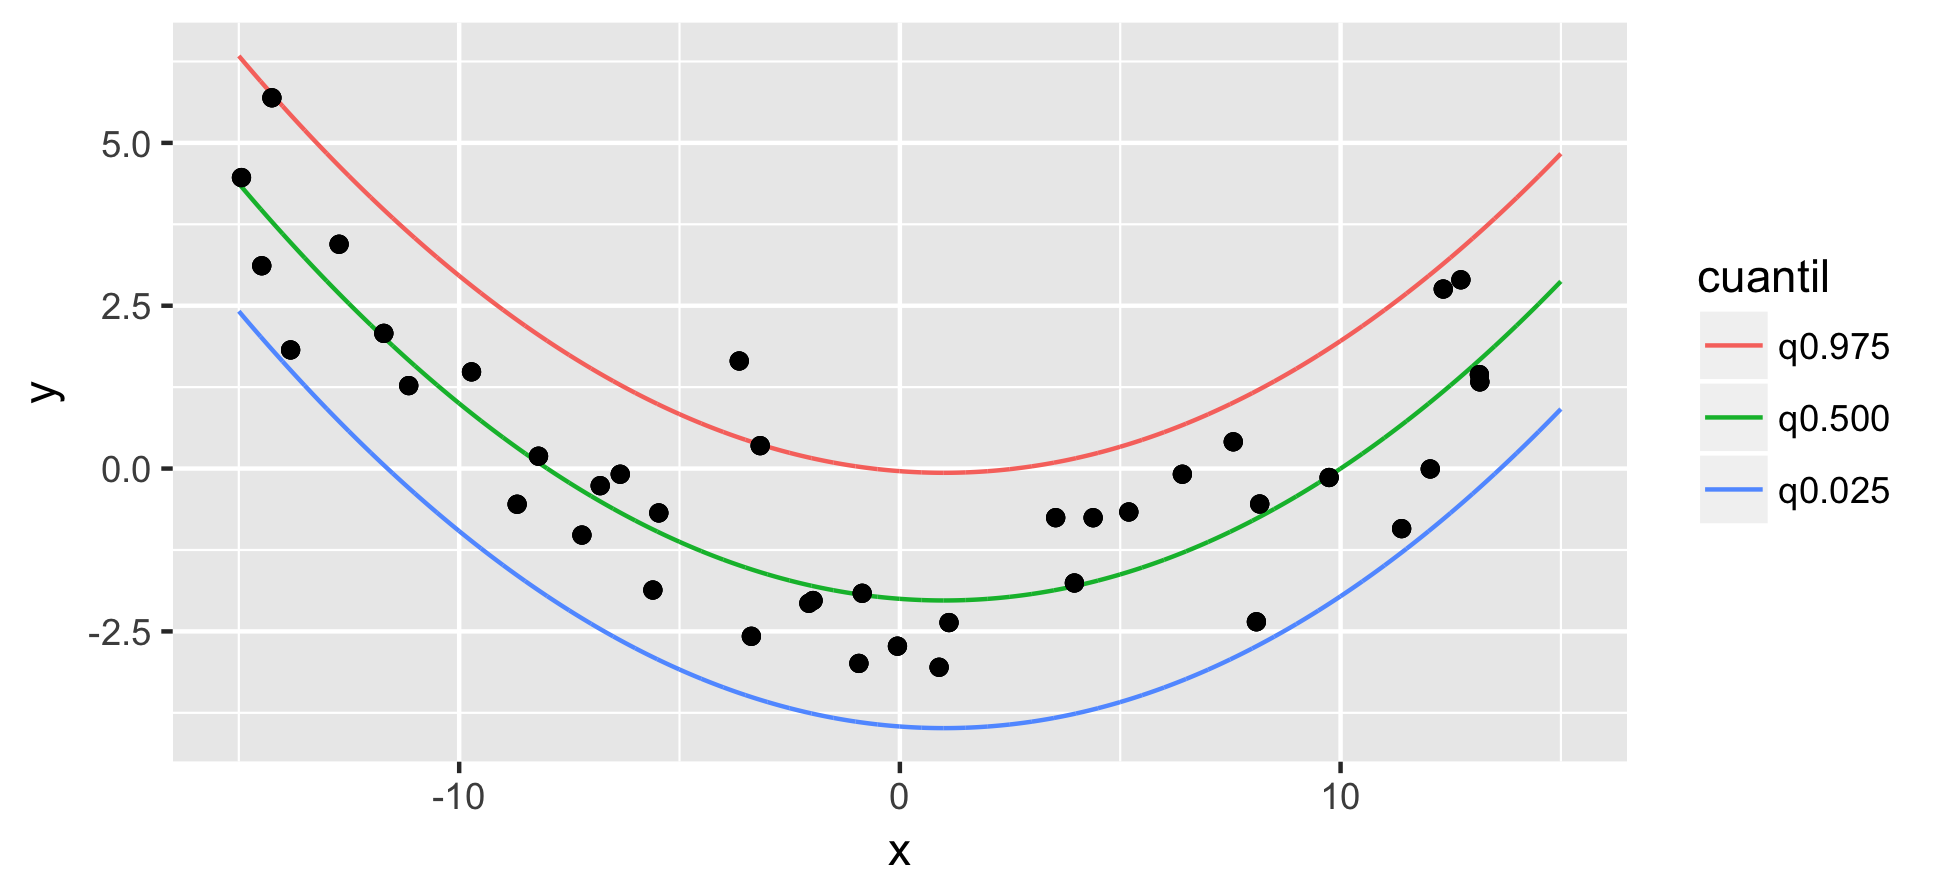
\includegraphics[width=0.60\textwidth]{Figures/Simulation/simple_g_simple_error/sample.png}
	\label{sample_sgse}
\end{figure}

\begin{figure}[H]
	\centering
	\caption{Ajuste del modelo \textit{GPDP}, para tendencia simple y dispersi\'on simple.}
	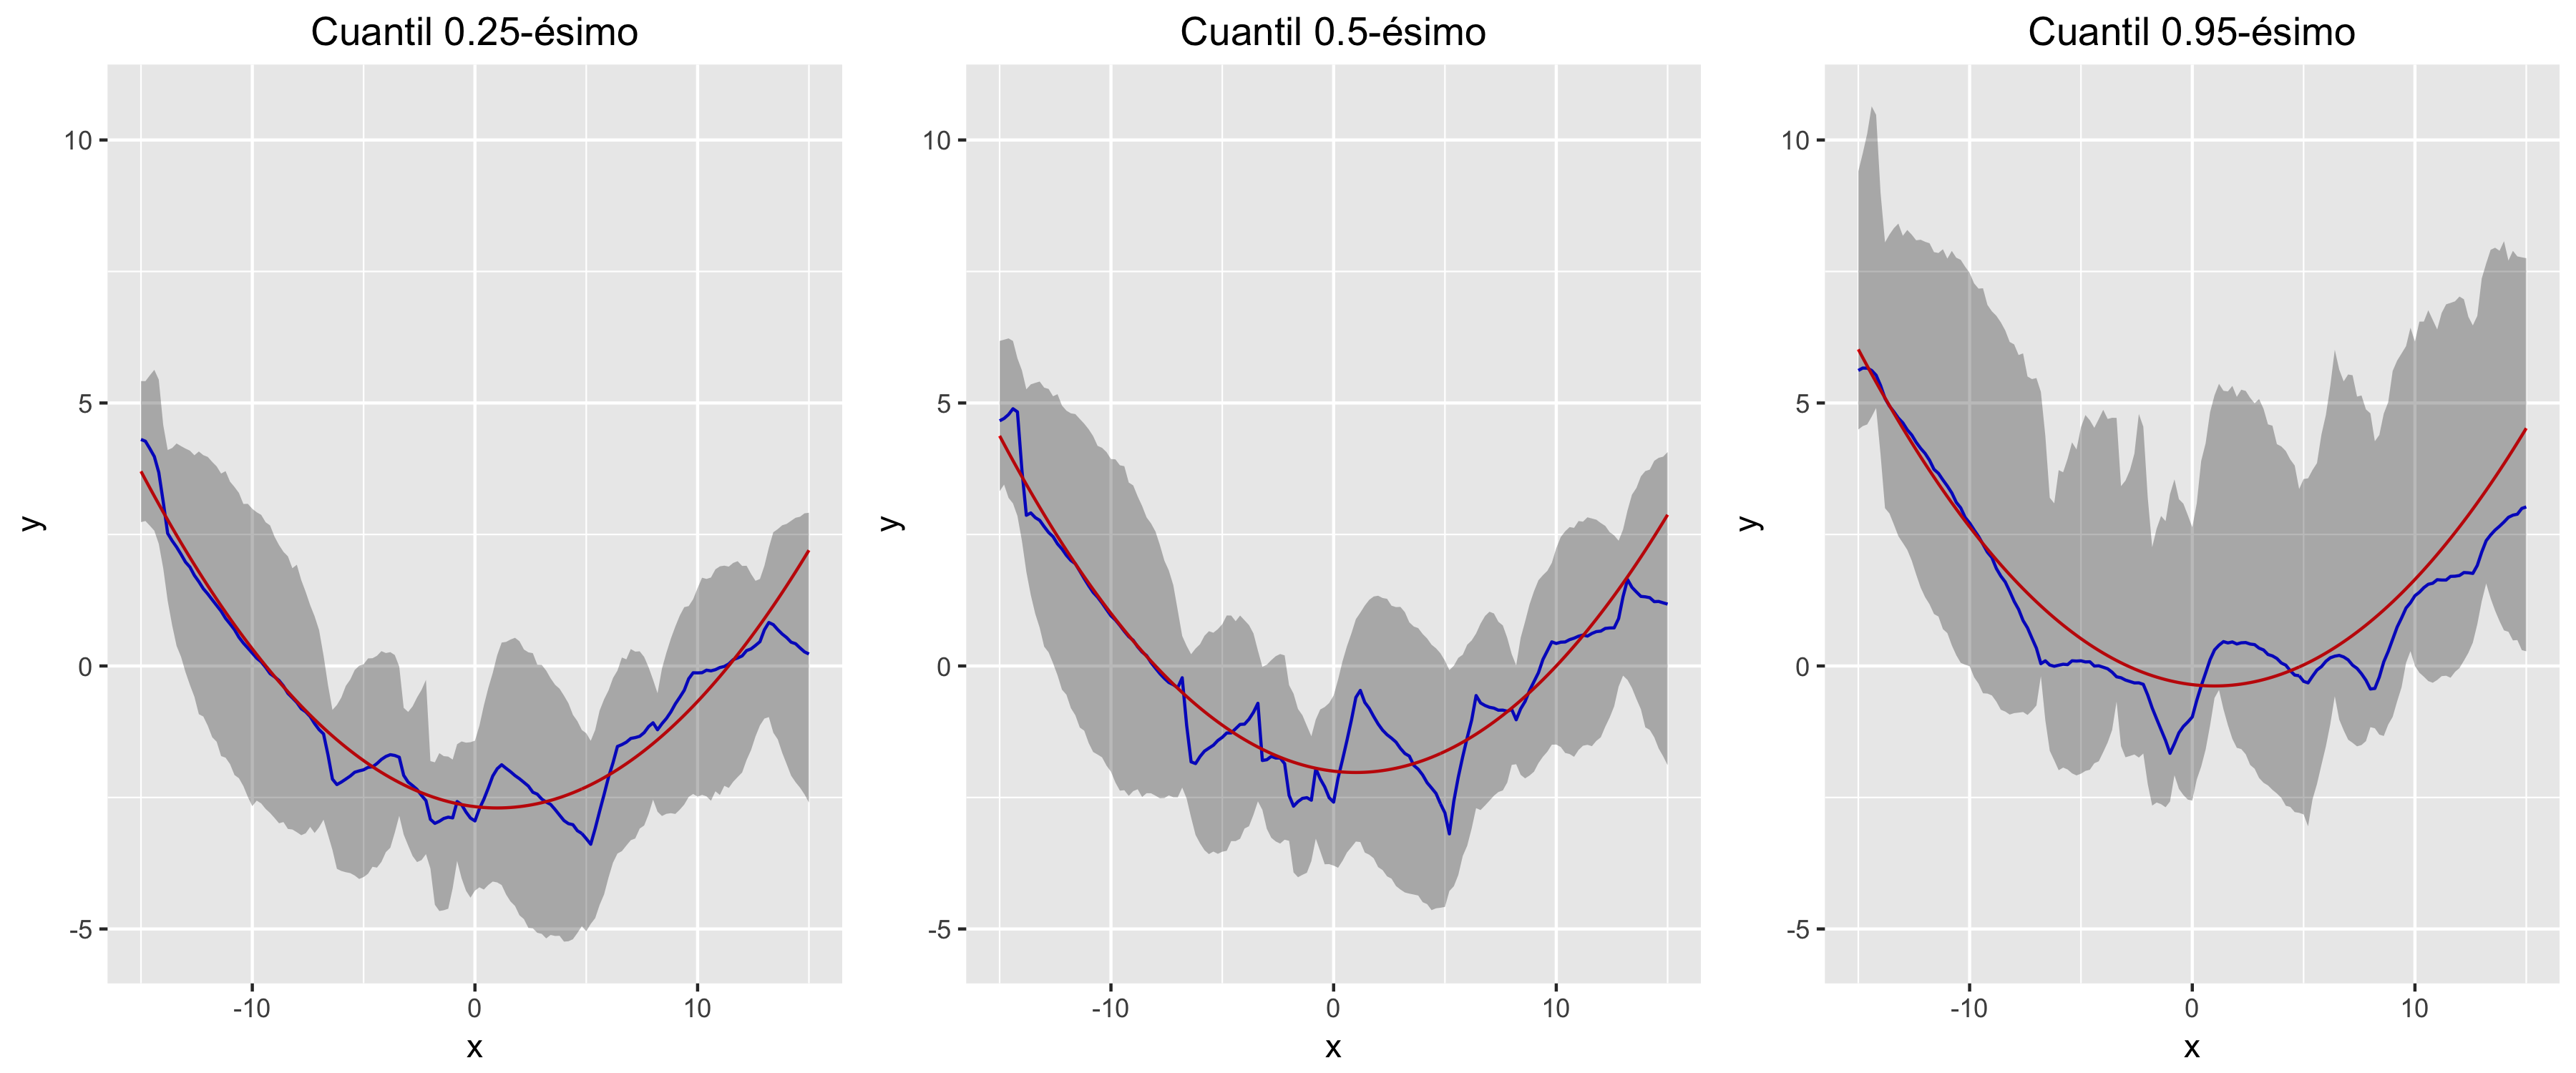
\includegraphics[width=\textwidth]{Figures/Simulation/simple_g_simple_error/fitted_models.png}
	\captionsetup{singlelinecheck=off,font=footnotesize}
    \caption*{Nota: La l\'inea roja representa el valor real de cada cuantil, la l\'inea azul representa la mediana de la distribuci\'on posterior predictiva y el \'area gris su intervalo de probabilidad al 90\%.}
	\label{fitted_sgse}
\end{figure}

Por otro lado, como se detall\'o en el cap\'itulo anterior, con el uso del paquete \textit{GPDPQuantReg} tambi\'en es posible algunos de los diagn\'osticos de las cadenas de Markov, los cuales se detallan en el \autoref{chap:MCMC}. Por ejemplo, se presentan los del cu\'antil $0.5$-\textit{\'esimo} en la figura \ref{diag_sgse}, mismos que reflejan un buen desempeño del algoritmo.

\begin{figure}[H]
	\centering
	\caption{Diagn\'osticos de las cadenas de Markov del cu\'antil $0.5$-\textit{\'esimo}, para tendencia simple y dispersi\'on simple.}
	\subfloat[Ergodicidad]{
	    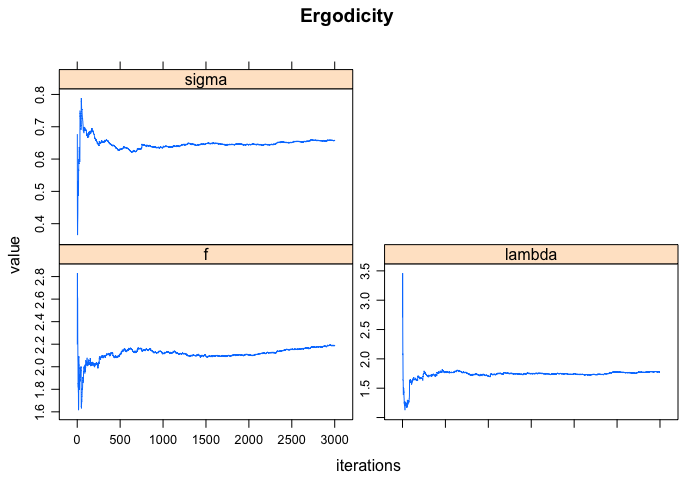
\includegraphics[width=0.45\textwidth]{Figures/Simulation/simple_g_simple_error/ergodicity.png}
	}
	\subfloat[Autocorrelaci\'on]{
	    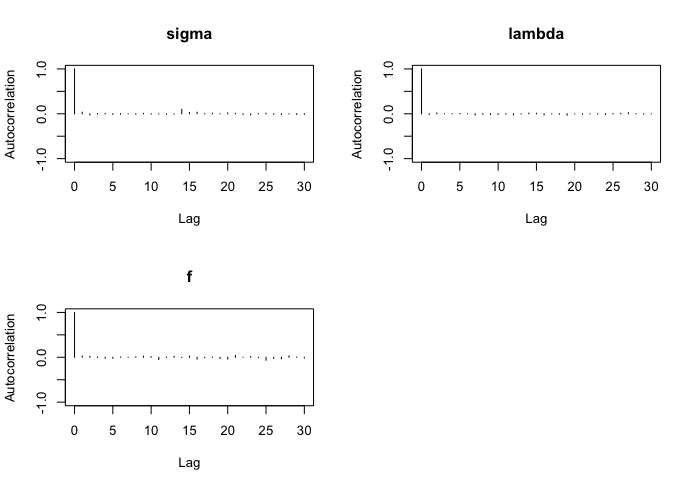
\includegraphics[width=0.45\textwidth]{Figures/Simulation/simple_g_simple_error/autocorrelation.png}
	}\\
	\subfloat[Correlaci\'on cruzada]{
	    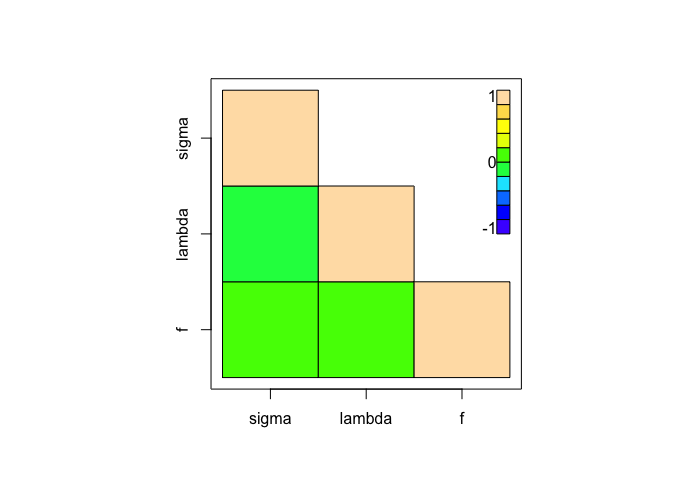
\includegraphics[width=0.45\textwidth]{Figures/Simulation/simple_g_simple_error/crosscorrelation.png}
	}
	\subfloat[Traza]{
	    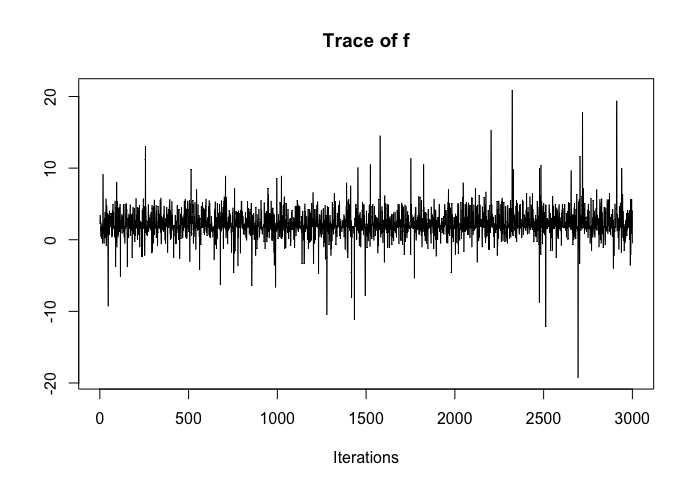
\includegraphics[width=0.45\textwidth]{Figures/Simulation/simple_g_simple_error/trace.png}
	}
	\label{diag_sgse}
\end{figure}

\subsection{Tendencia compleja, dispersi\'on simple}

En este caso, se mantuvo que $E \sim \mathcal{N}(1,0)$, pero la tendencia $g$ usada fue m\'as compleja:
\begin{equation*}
    g(x) = \frac{1}{2} x \cos(x) - \exp\left(\frac{1}{10}x\right).
\end{equation*}

Los datos simulados se pueden observar en la figura \ref{sample_cgse}, los cuales al ajustar el modelo mostraron de nuevo buenos resultados (figura \ref{fitted_cgse}), apareciendo la tendencia original adentro del intervalo de probabilidad al 90\% en pr\'acticamente todos los valores de $x$ en los que se realiz\'o predicci\'on, a excepci\'on de la \'ultima zona, en la que no hubo datos de entrenamiento.

\begin{figure}[H]
	\centering
	\caption{Datos simulados y cuantiles de referencia, para tendencia compleja y dispersi\'on simple.}
	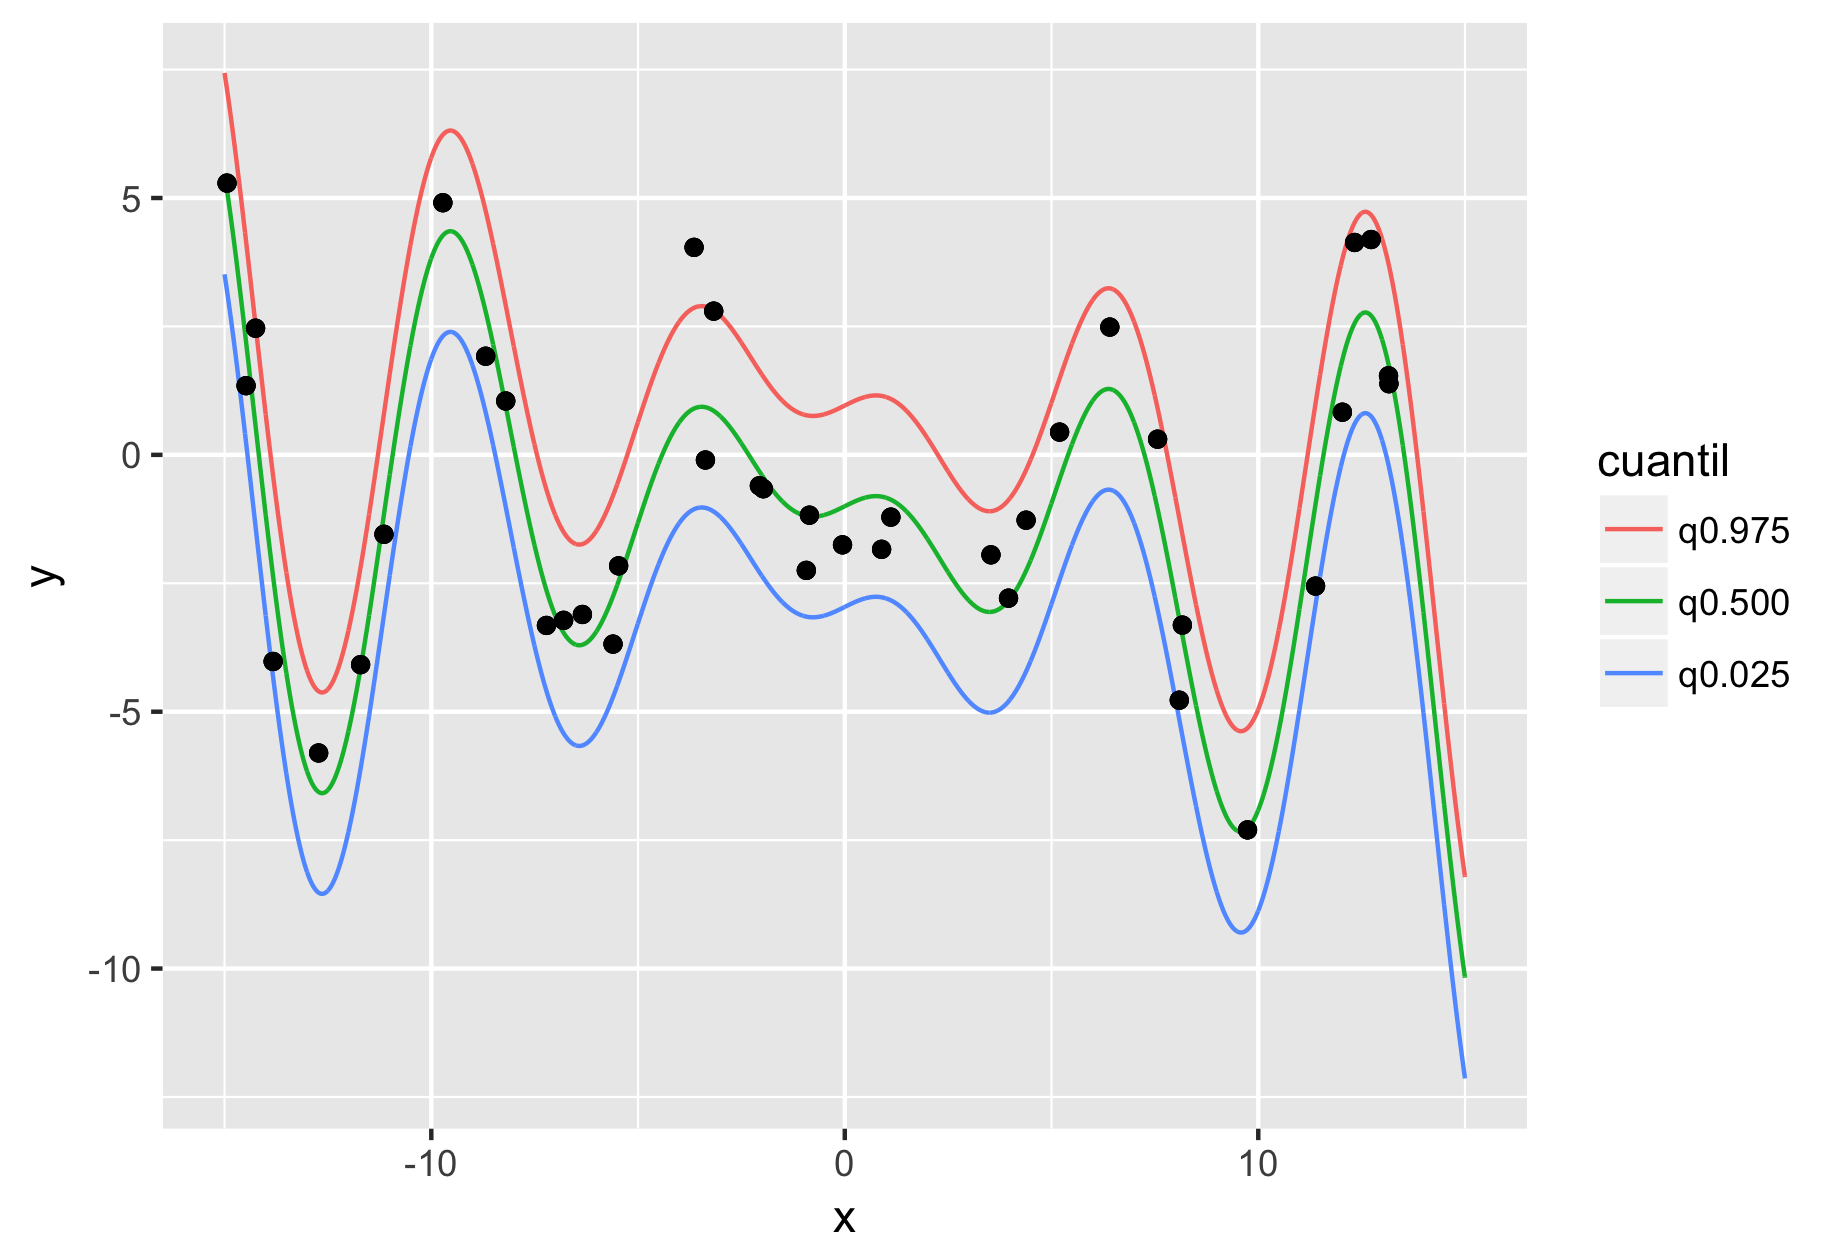
\includegraphics[width=0.60\textwidth]{Figures/Simulation/complex_g_simple_error/sample.png}
	\label{sample_cgse}
\end{figure}

\begin{figure}[H]
	\centering
	\caption{Ajuste del modelo \textit{GPDP}, para tendencia compleja y dispersi\'on simple.}
	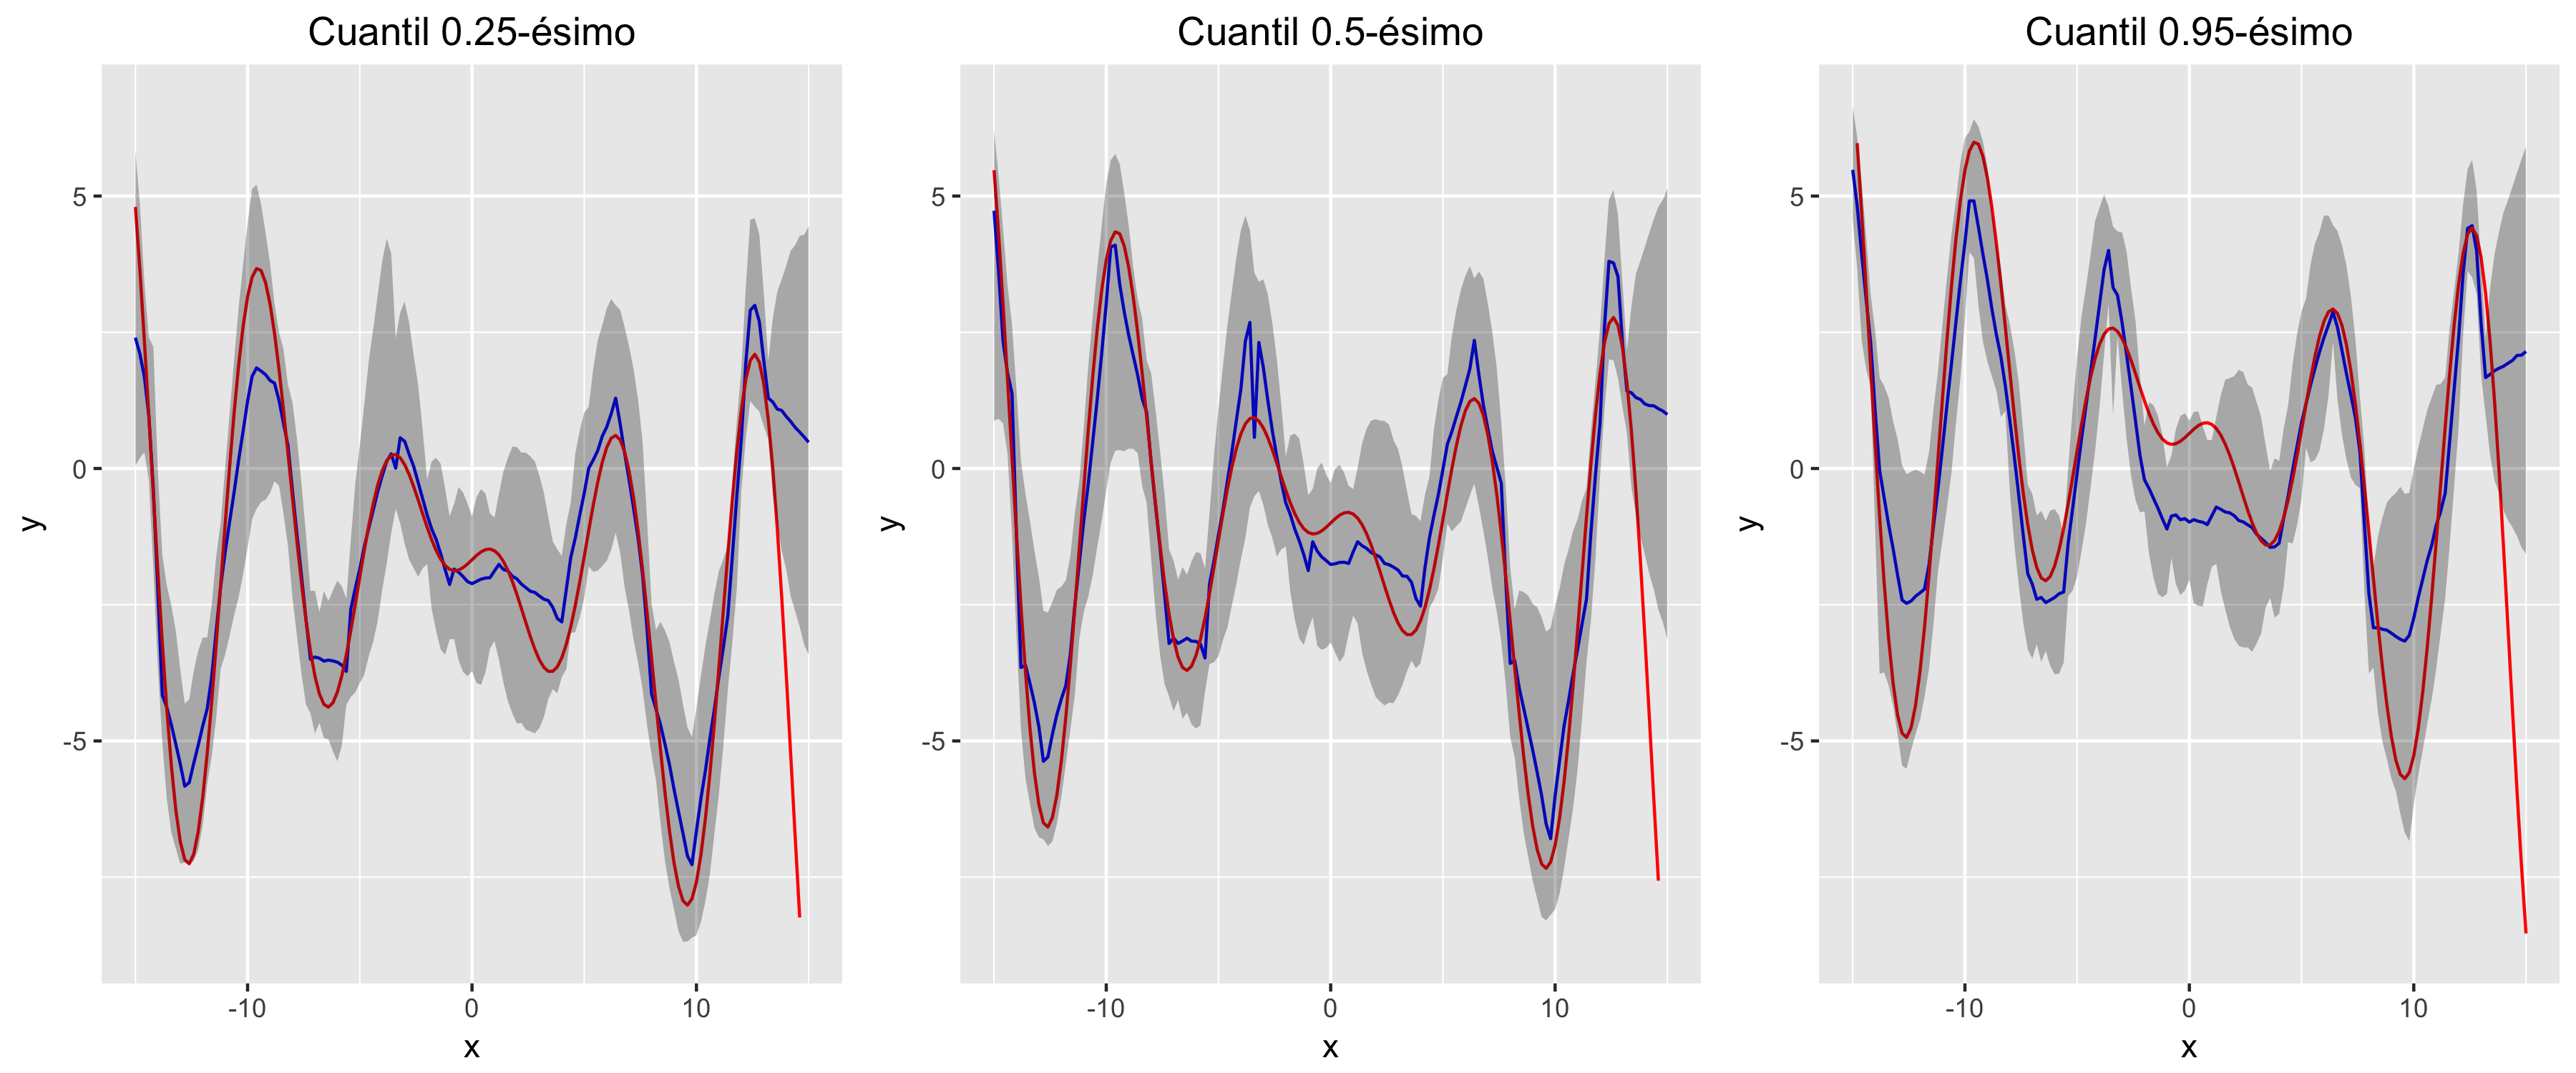
\includegraphics[width=\textwidth]{Figures/Simulation/complex_g_simple_error/fitted_models.png}
	\captionsetup{singlelinecheck=off, font=footnotesize}
    \caption*{Nota: La l\'inea roja representa el valor real de cada cuantil, la l\'inea azul representa la mediana de la distribuci\'on posterior predictiva y el \'area gris su intervalo de probabilidad al 90\%.}
	\label{fitted_cgse}
\end{figure}

\subsection{Tendencia simple, dispersi\'on compleja}

En este caso, se uso la tendencia lineal:
\begin{equation*}
    g(x) = \frac{1}{2} x.
\end{equation*}
La complejidad se introdujo en $E \sim \textit{Gamma}(\alpha = 2,\beta = 1)$, debido a que la dipersi\'on no fue sim\'etrica y fue acotada por la izquierda. 

El conjunto de datos usado para este modelo aparece en la figura \ref{sample_sgce}, y a pesar de la complejidad de la dispersi\'on, se obtuvieron buenos resultados (figura \ref{fitted_sgce}), debido a que nuevamente las funciones reales de los diversos cuantiles cayeron en su totalidad dentro del intervalo de probabilidad al 90\%, estimado por el modelo.

Un detalle notable es que, al igual que el caso de tendencia simple y dispersi\'on simple, la estimaci\'on de la funci\'on del cuantil 0.95\textit{-\'esimo} muestra una varianza m\'as grande que los otros dos cuantiles. Esto debido a que en valores extremos el modelo refleja mayor incertidumbre de lo que en realidad podr\'ia estar ocurriendo.

\begin{figure}[H]
	\centering
	\caption{Datos simulados y cuantiles de referencia, para tendencia simple y dispersi\'on compleja.}
	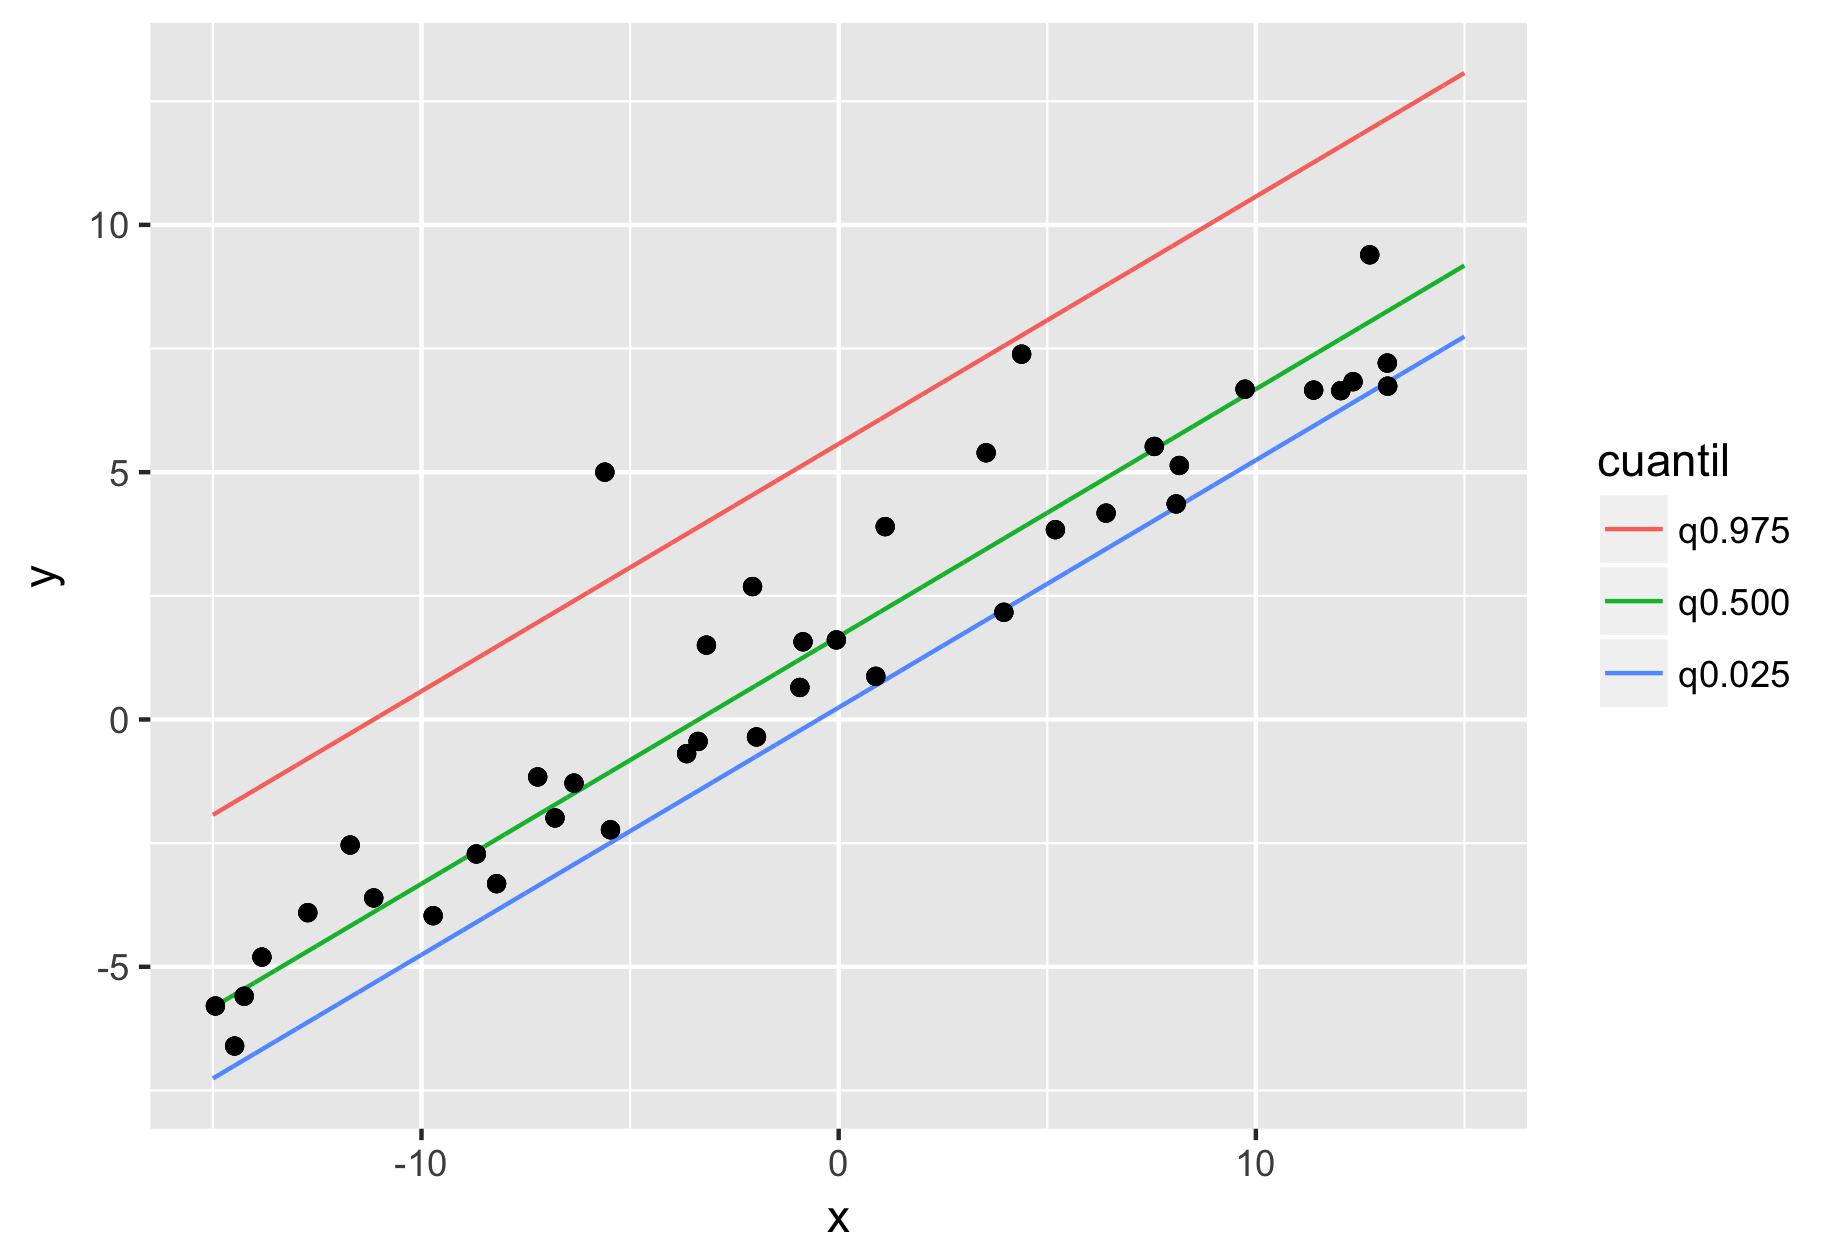
\includegraphics[width=0.60\textwidth]{Figures/Simulation/simple_g_complex_error/sample.png}
	\label{sample_sgce}
\end{figure}

\begin{figure}[H]
	\centering
	\caption{Ajuste del modelo \textit{GPDP}, para tendencia simple y dispersi\'on compleja.}
	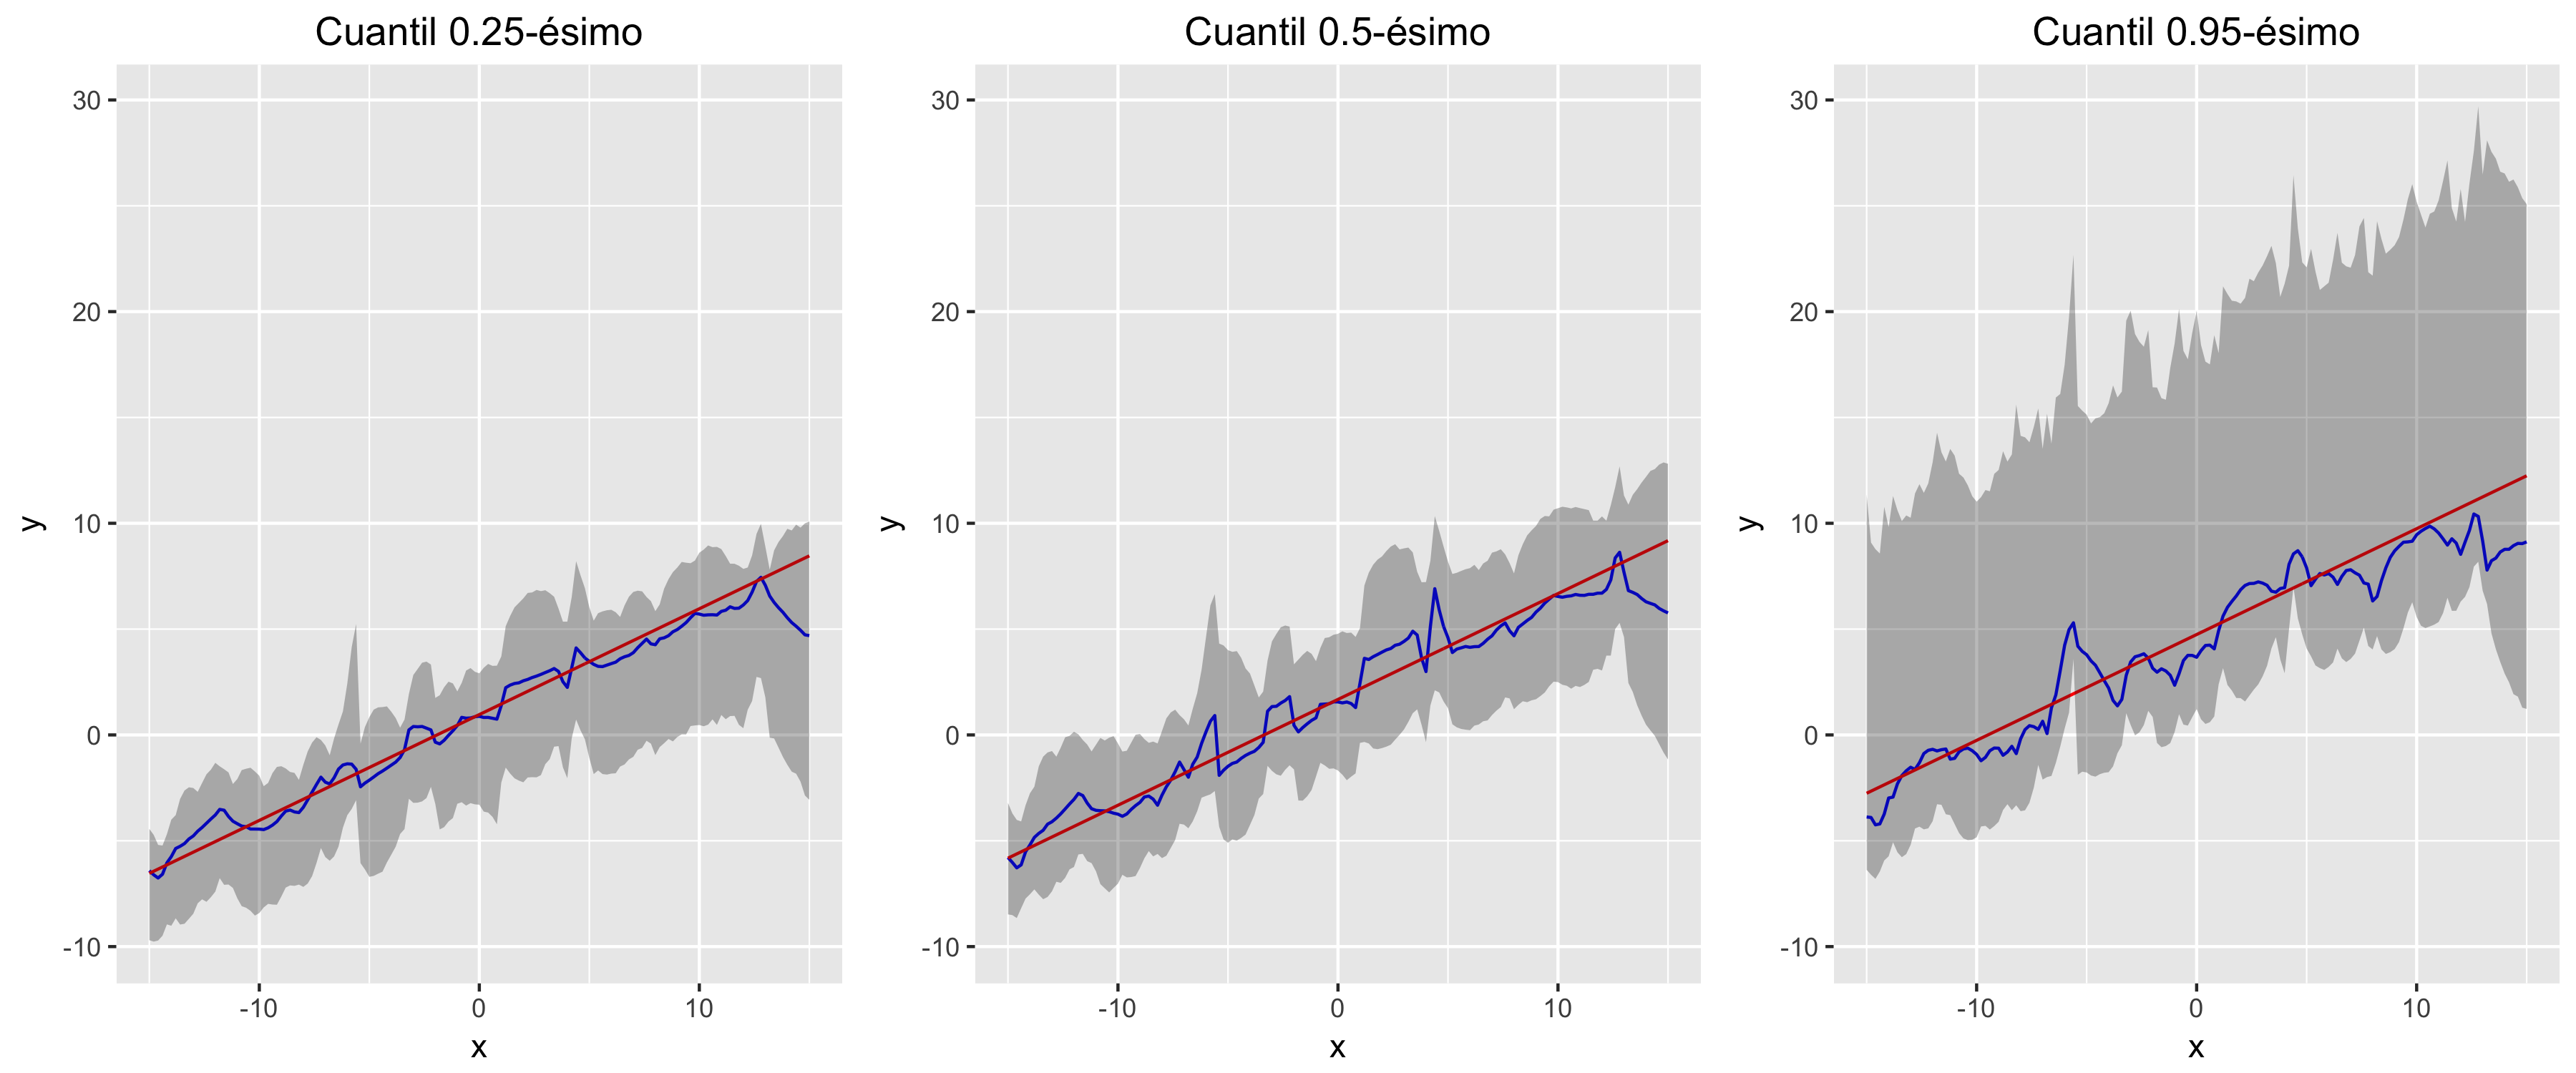
\includegraphics[width=\textwidth]{Figures/Simulation/simple_g_complex_error/fitted_models.png}
	\captionsetup{singlelinecheck=off,font=footnotesize}
    \caption*{Nota: La l\'inea roja representa el valor real de cada cuantil, la l\'inea azul representa la mediana de la distribuci\'on posterior predictiva y el \'area gris su intervalo de probabilidad al 90\%.}
	\label{fitted_sgce}
\end{figure}

\subsection{Tendencia compleja, dispersi\'on compleja}

En este modelo se usaron datos (figura \ref{sample_cgce}) provenientes tanto de una dispersi\'on compleja, $E \sim \textit{Gamma}(\alpha = 2,\beta = 1)$, como de una tendencia $g$ compleja:
\begin{equation*}
    g(x) = \frac{1}{2} x \cos(x) - \exp\left(\frac{1}{10}x\right).
\end{equation*}

Despu\'es del ajuste (figura \ref{fitted_cgce}), el balance fue positivo, debido a que las funciones reales de los diversos cuantiles cayeron en su totalidad dentro del intervalo de probabilidad al 90\%, del estimado por el modelo, a excepci\'
on de la zona de la que no se tuvieron datos, como en el caso de tendencia compleja y dispersi\'on simple. Pero a diferencia de ese modelo, la dispersi\'on compleja produce una mayor incertidumbre, particularmente notoria en el caso del cuantil 0.95\textit{-\'esimo}.

\begin{figure}[H]
	\centering
	\caption{Datos simulados y cuantiles de referencia, para tendencia compleja y dispersi\'on compleja.}
	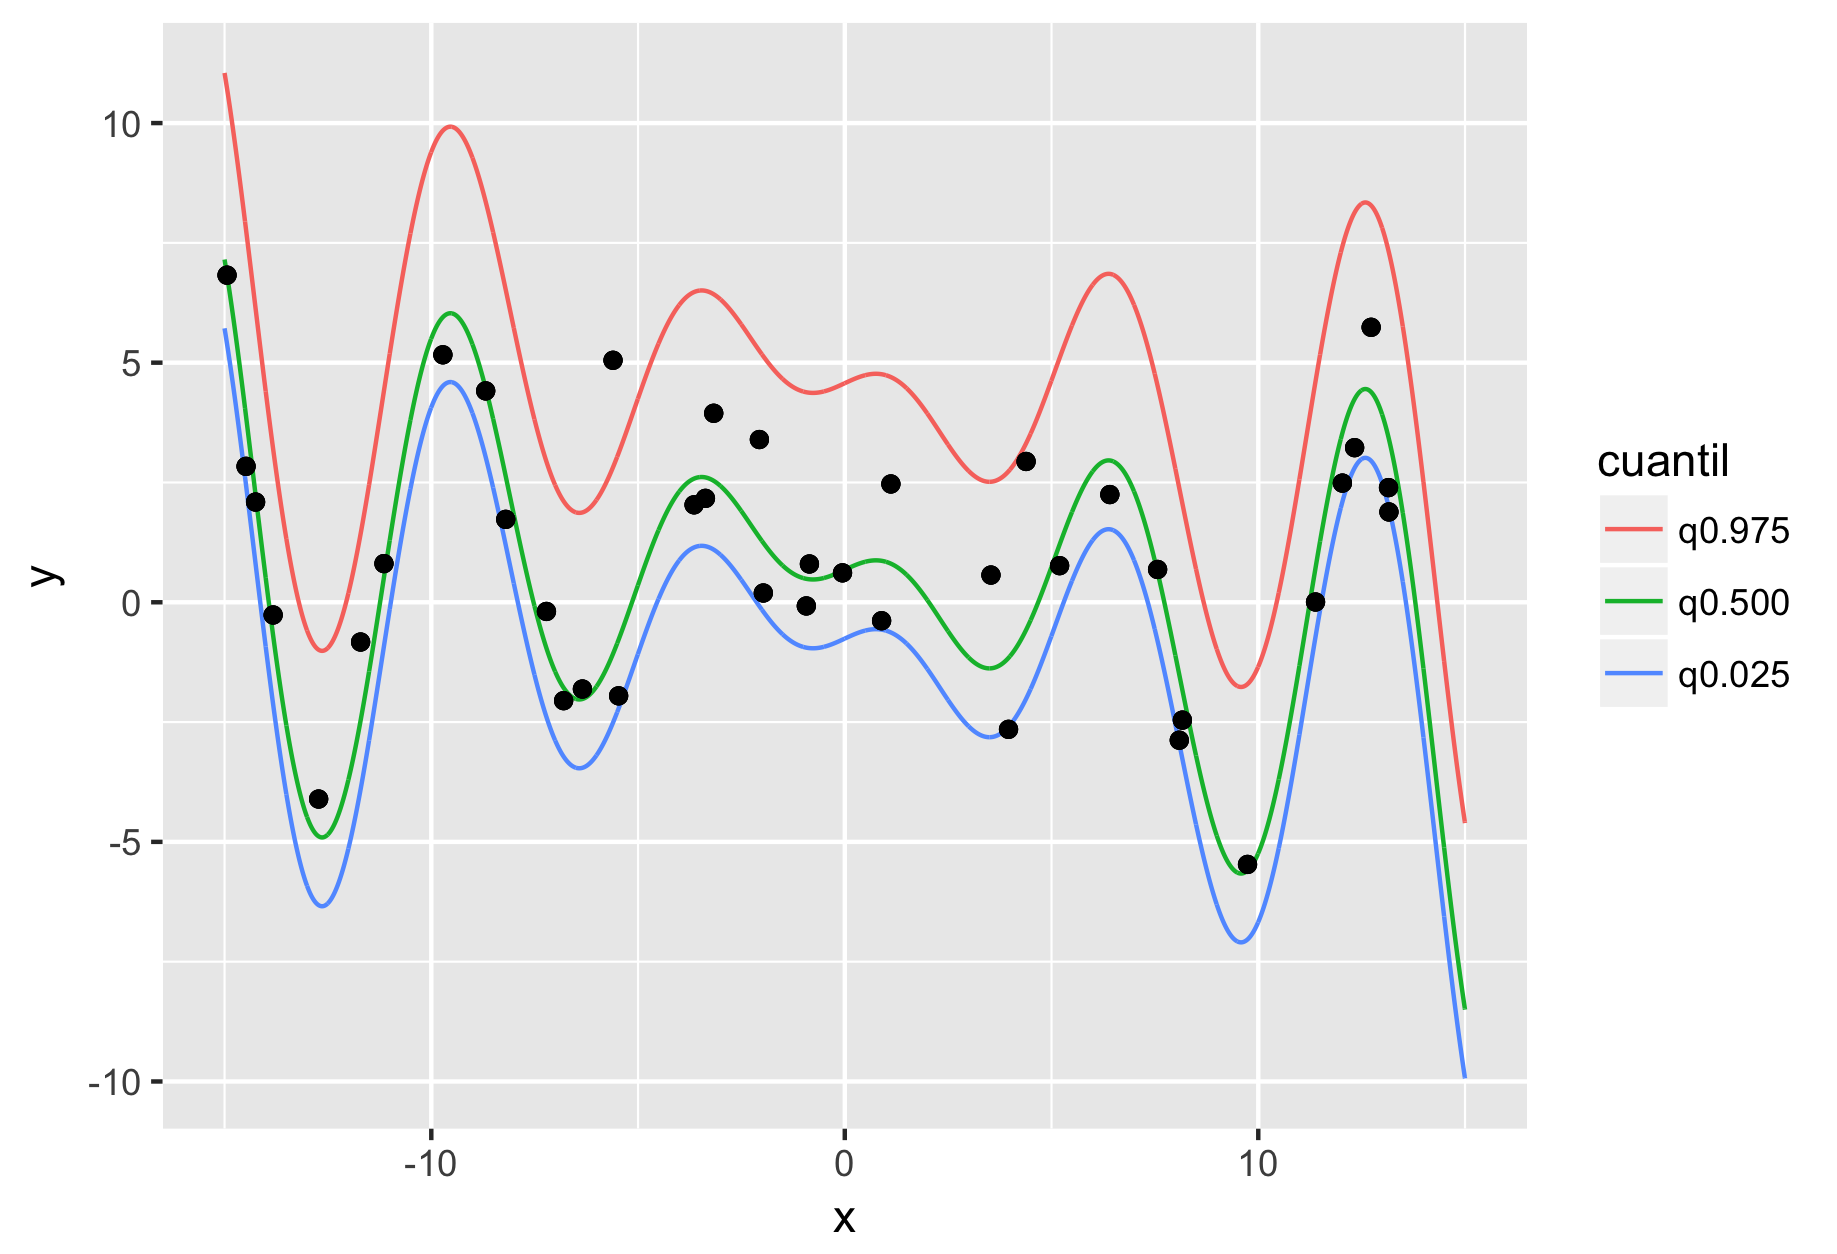
\includegraphics[width=0.60\textwidth]{Figures/Simulation/complex_g_complex_error/sample.png}
	\label{sample_cgce}
\end{figure}

\begin{figure}[H]
	\centering
	\caption{Ajuste del modelo \textit{GPDP}, para tendencia compleja y dispersi\'on compleja.}
	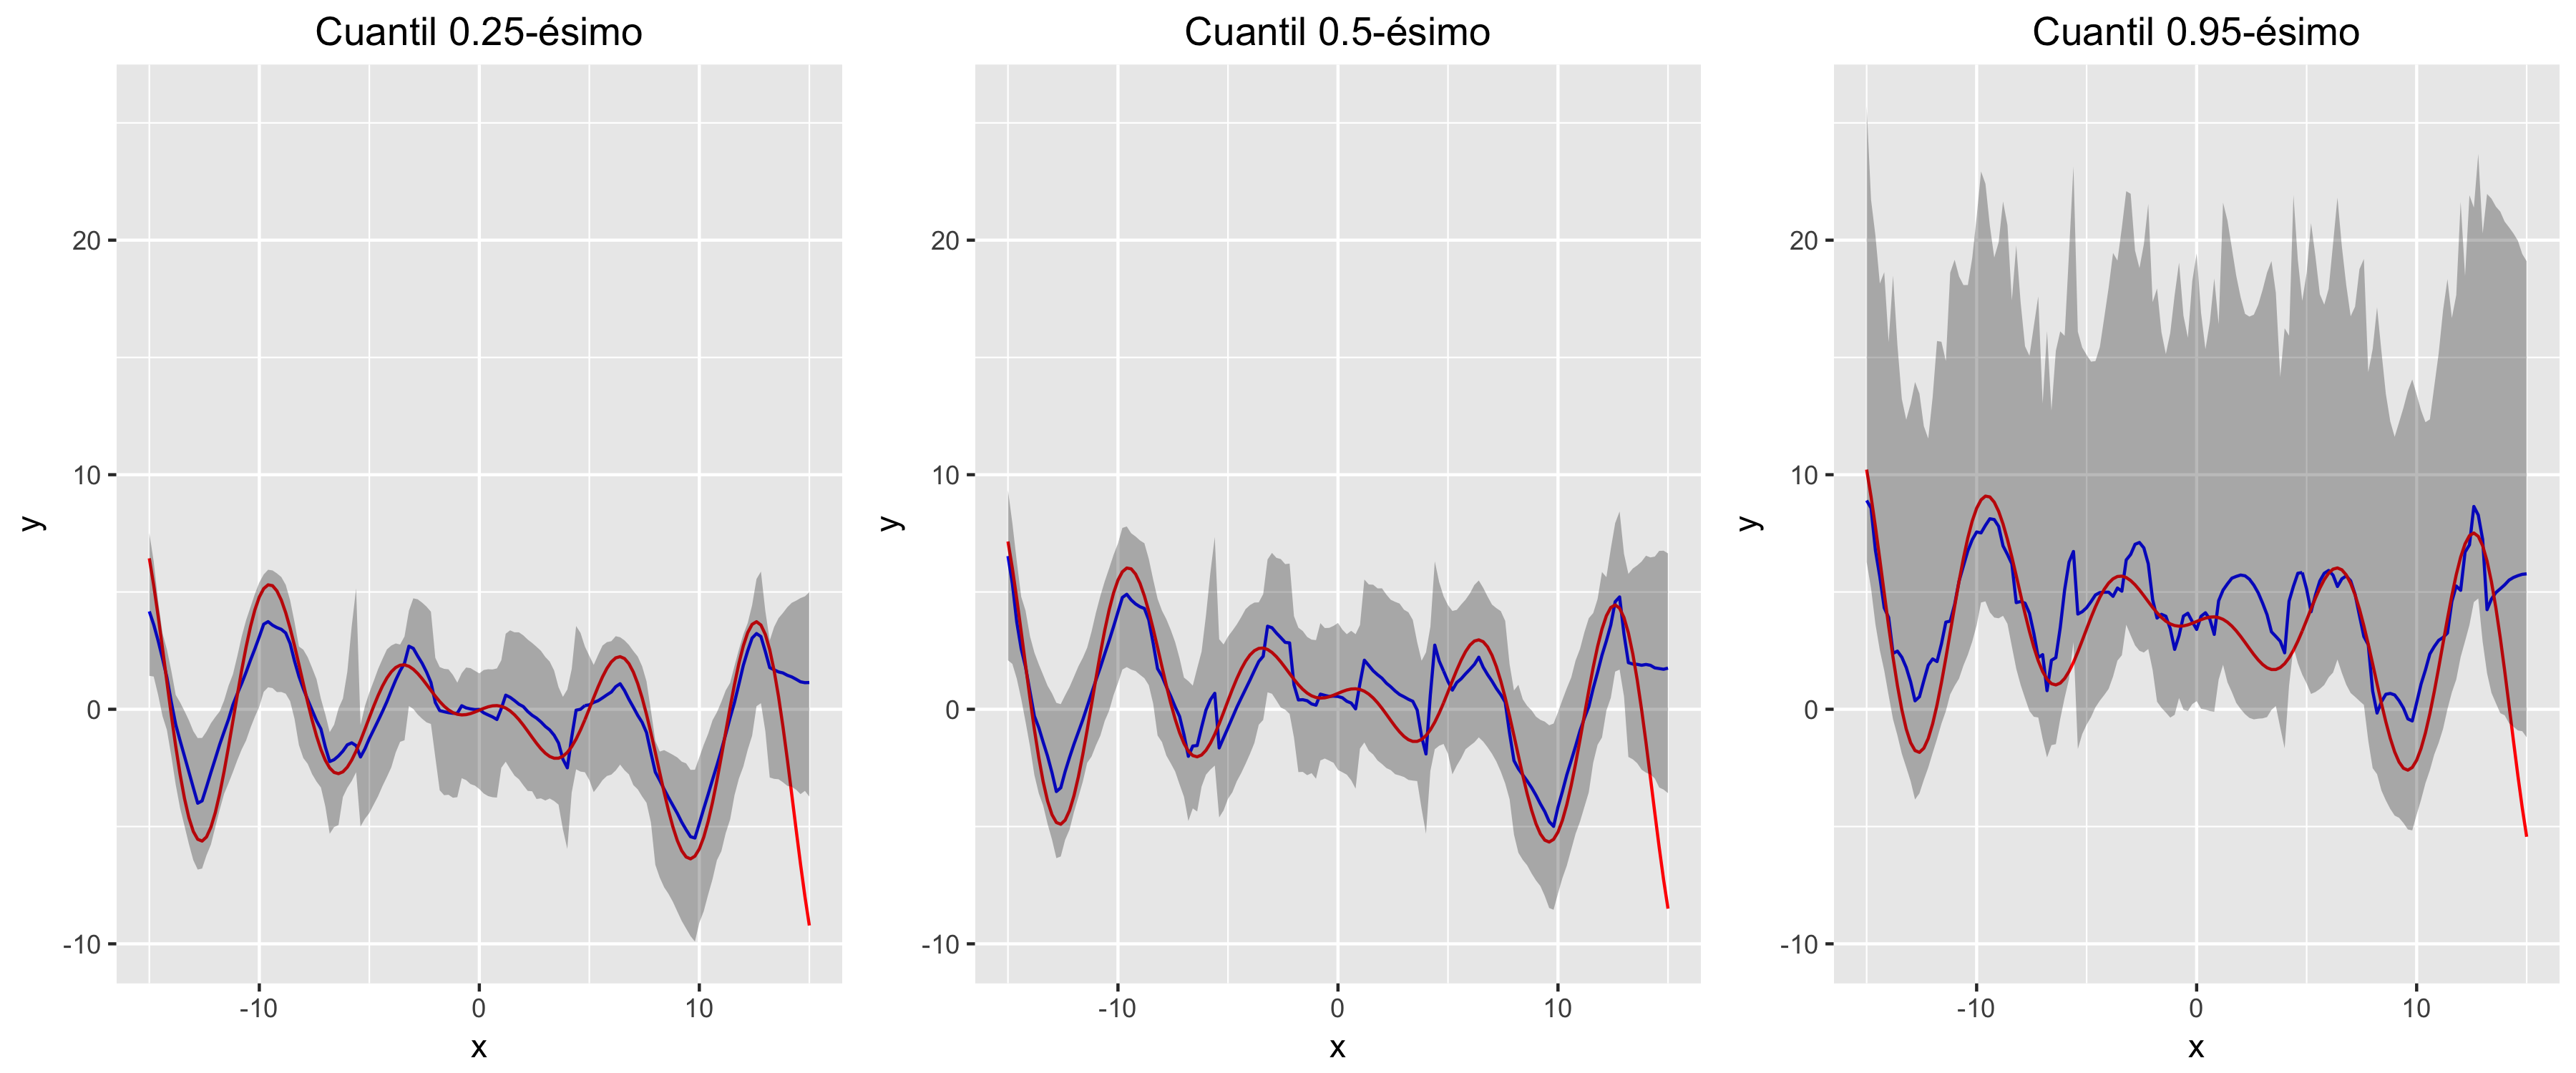
\includegraphics[width=\textwidth]{Figures/Simulation/complex_g_complex_error/fitted_models.png}
	\captionsetup{singlelinecheck=off,font=footnotesize}
    \caption*{Nota: La l\'inea roja representa el valor real de cada cuantil, la l\'inea azul representa la mediana de la distribuci\'on posterior predictiva y el \'area gris su intervalo de probabilidad al 90\%.}
	\label{fitted_cgce}
\end{figure}

Una vez corroborado que el modelo funciona bien con datos simulados, a continuaci\'on se presentan los resultados de su aplicaci\'on a un problema real, dentro de las tareas laborales del autor.

\section{Investigaci\'on de mercados}

\subsection{Conceptos iniciales}

En el contexto de la investigaci\'on de mercados una de las m\'etricas que se consideran m\'as importantes es la del \textit{Conocimiento de marca}, misma que se define como el porcentaje de una cierta poblaci\'on que declara conocer el nombre de la marca en cuesti\'on.

Dentro de dicho ambiente, la teor\'ia dice que esa m\'etrica normalmente depende de la publicidad pautada semana a semana. Cuando una marca \'unicamente se publicita en televisi\'on, el valor com\'unmente usado para medir esa inversi\'on se denomina \textit{Adstocked GRP}s, y, en esencia, se compone de cu\'antas veces se transmiti\'o el comercial y cu\'anta gente estaba viendo la televisi\'on cuando se transmiti\'o,  ponderado por qu\'e tan lejana en el tiempo sucedi\'o dicha transmisi\'on, respecto al d\'ia de hoy. Asimismo, tambi\'en se suelen usar las inversiones de los competidores para explicar el \textit{Conocimiento de marca}, debido a que es com\'un que las personas se confundan y asocien a la marca un comercial del competidor.

En el pasado, inversiones iguales han representado resultados ligeramente distintos en los niveles de \textit{Conocimiento de marca}, volatilidad que normalmente es asociada a la calidad de los comerciales, tanto los propios, como los del competidor. En otras palabras, comerciales m\'as memorables han generado un mayor \textit{Conocimiento de marca} a la que los pauta, y una aportaci\'on muy pequeña al competidor, cuando se han transmitido en aproximadamente la misma cantidad ocasiones y a una similar audiencia.

Adem\'as, tambi\'en es importante revisar el concepto de \textit{marca madre} y \textit{subvariantes}, para nuestra siguiente aplicaci\'on del modelo GPDP. Una \textit{marca madre} es aquella que tiene fama por su propio nombre, pero que se ofrece al consumidor mediante productos (tambi\'en llamados \textit{subvariantes}) que son publicitados por s\'i solos. Por ejemplo, se puede pensar en la empresa de tecnolog\'ia \textit{Pera} que tiene comerciales que posicionan su nombre, pero tiene tambi\'en comerciales donde promociona \'unicamente el celular que producen, y en otros, \'unicamente la tableta.

Dicho esto, normalmente se piensa que los comerciales de la \textit{marca madre} contribuyen m\'as al \textit{Conocimiento de marca} que aquellos de las \textit{subvariantes}, que tienen como prop\'osito vender los productos espec\'ificos, m\'as que posicionar la marca.

\subsection{Caso real}

Cierta \textit{marca madre} es cliente de la empresa de investigaci\'on de mercados en la que sol\'ia trabajar. Dicha marca registr\'o semana a semana los valores de inversi\'on en los comerciales que buscaban posicionar su nombre, los realizados para los de sus \textit{subvariantes}, los de su competencia y el \textit{Conocimiento de marca} reportado durante 2014 y 2015. Estos sirvieron para entrenar un modelo GPDP, bajo el supuesto que las mediciones semanales fueron independientes condicionalmente a la inversi\'on. Los valores predichos por el GPDP comparados contra los que en efecto se observaron se presentan a continuaci\'on.

\begin{figure}[H]
	\centering
	\caption{Modelo de \textit{Conocimiento de marca} para datos de entrenamiento (2014-2015).}
	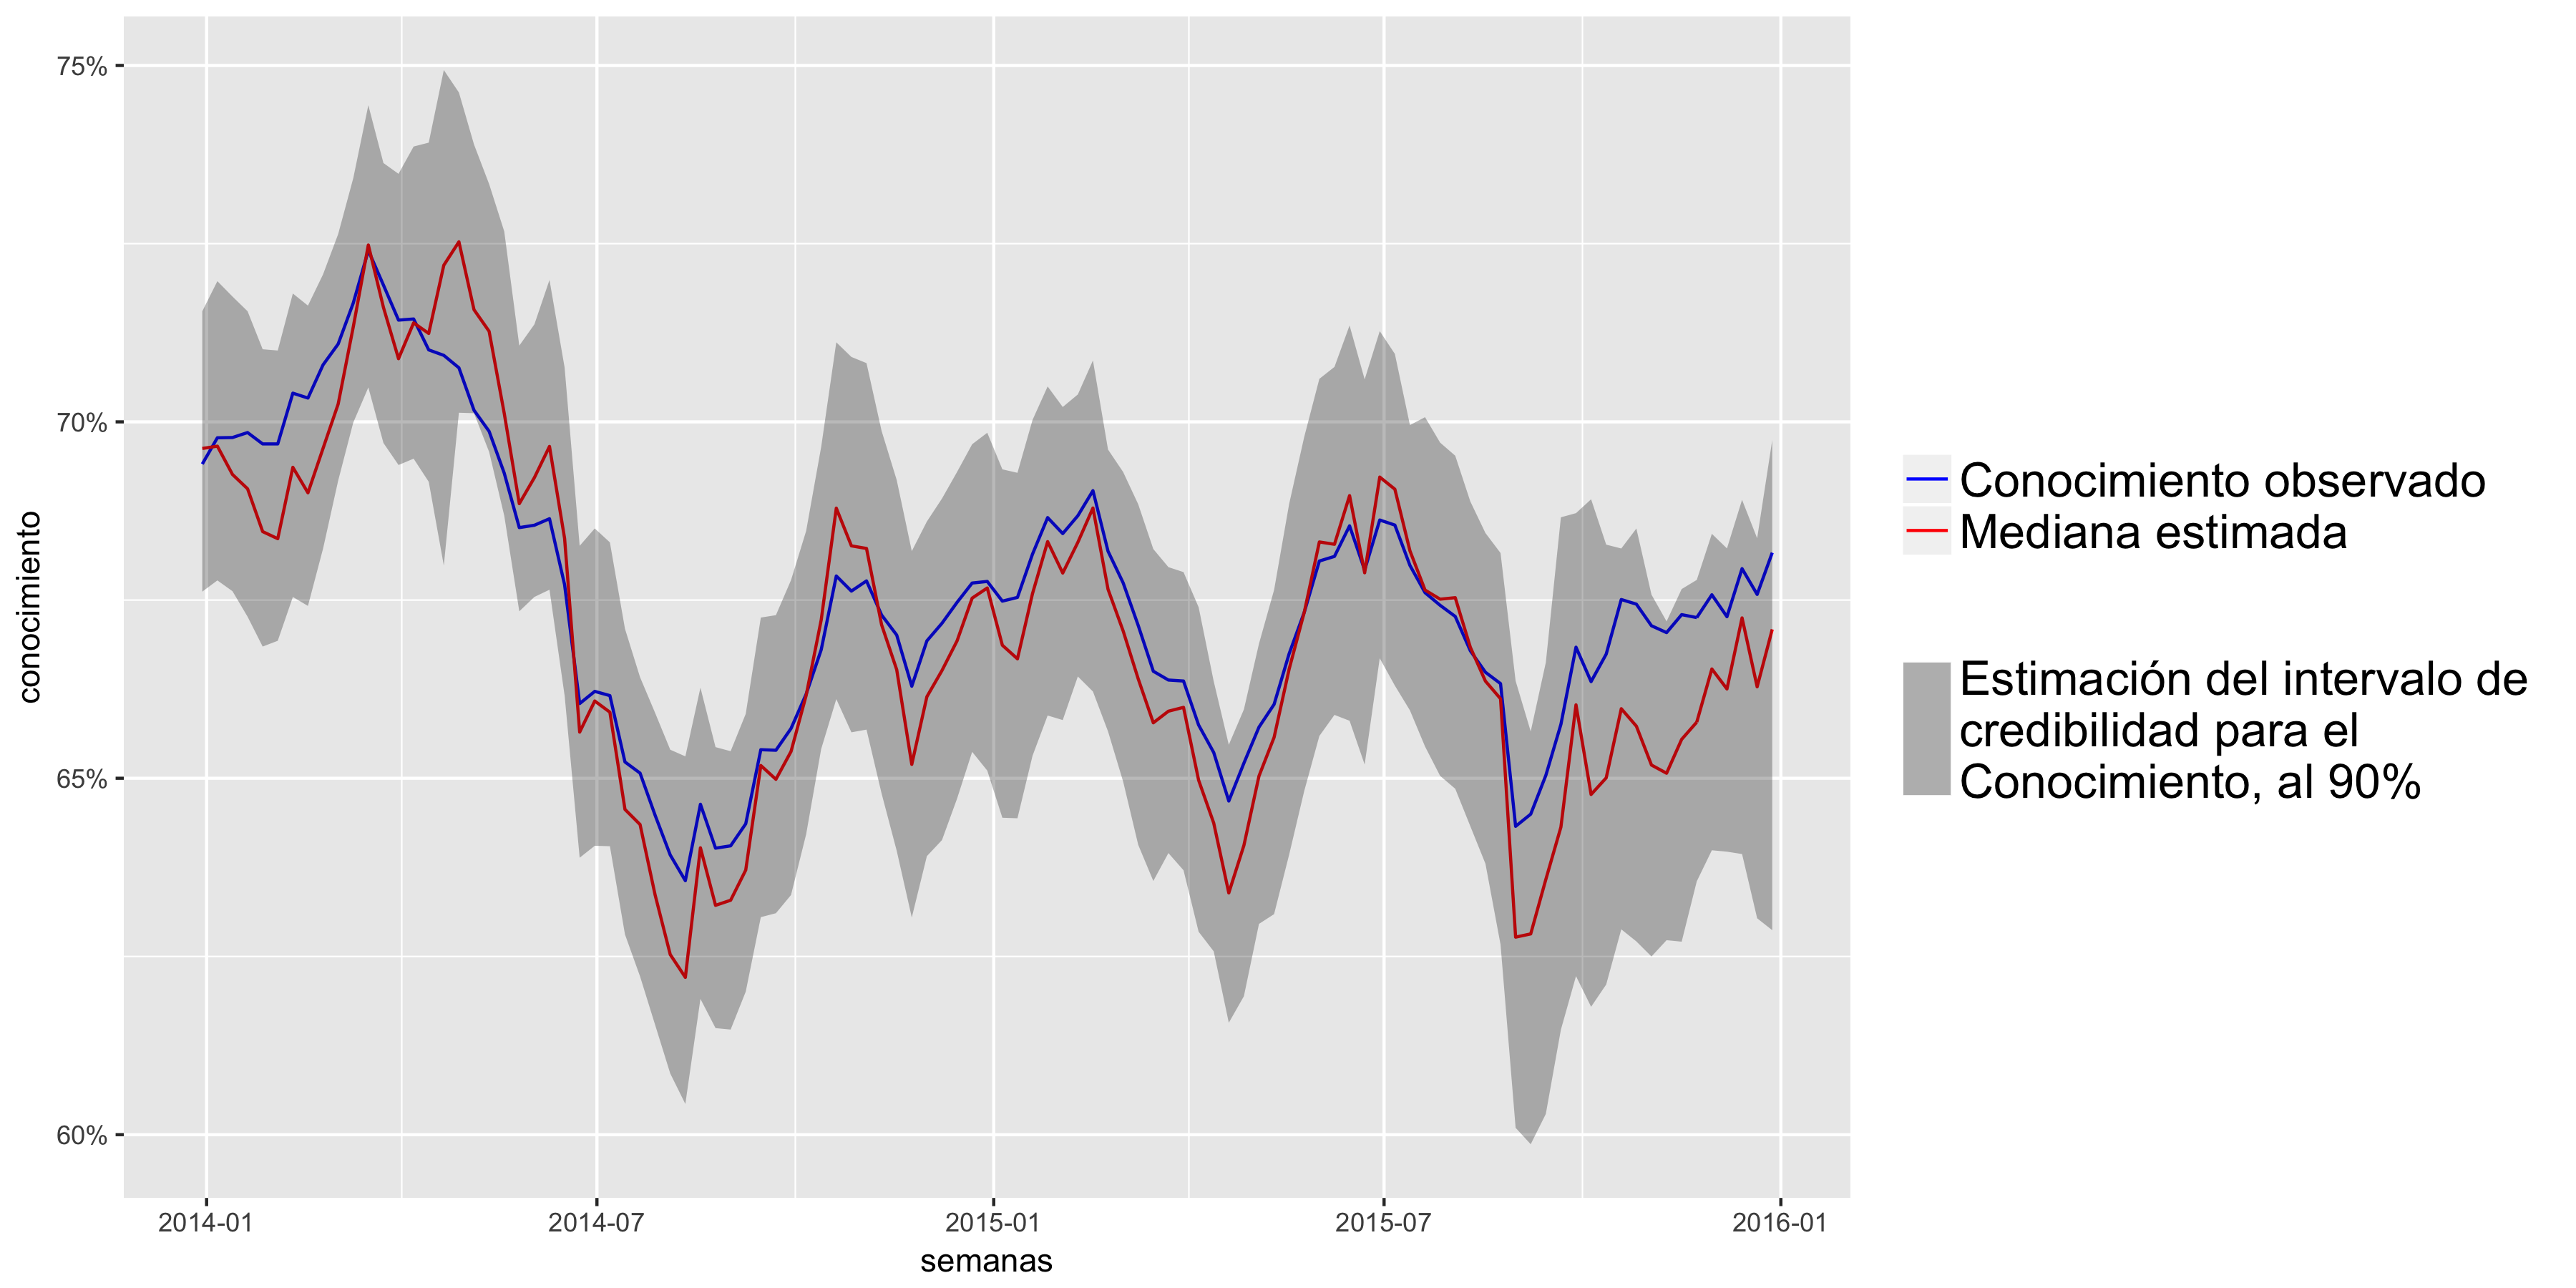
\includegraphics[width=1\textwidth]{Figures/MarketResearch/fit_review.png}
	\captionsetup{singlelinecheck=off,font=footnotesize}
	\caption*{Nota: El intervalo de credibilidad se construy\'o usando las estimaciones de la mediana de los cuantiles $0.05$-\'esimo y $0.95$-\'esimo.}
	\label{awareness_fit}
\end{figure}

Es verificable que el \textit{Conocimiento de marca} sigue un movimiento muy similar a la mediana que predijo el modelo durante el primer año y medio, y, de hecho, en los \'ultimos se ha despegado positivamente.

Todo lo anterior se hizo ignorando el hecho de que tambi\'en se ten\'ian los datos de 2016, con la intenci\'on de ver c\'omo funcionar\'ia el modelo. Al cliente particularmente le interesaba ver esto porque la m\'etrica tuvo una estrepitosa ca\'ida durante el 2016 y ten\'ia la duda si era por una estrategia desafortunada de su inversi\'on o por el hecho de que su competidor hab\'ia cambiado completamente el concepto de sus comerciales, situaci\'on que podr\'ia estar provocando que la gente ya no se confundiera y los relacionara err\'oneamente a los de la marca de nuestro cliente.

Traslado al lenguaje del modelo, se deseaba ver si el valor realmente observado pudo haber sido predicho por el modelo o si lo consideraba poco probable, situaci\'on en la que efectivamente se podr\'ia hablar de un cambio estructural ocurrido dentro de este contexto. Los resultados obtenidos fueron los siguientes.

\begin{figure}[H]
	\centering
	\caption{\textit{Conocimiento de marca} en 2016, comparado con el modelo GPDP.}
	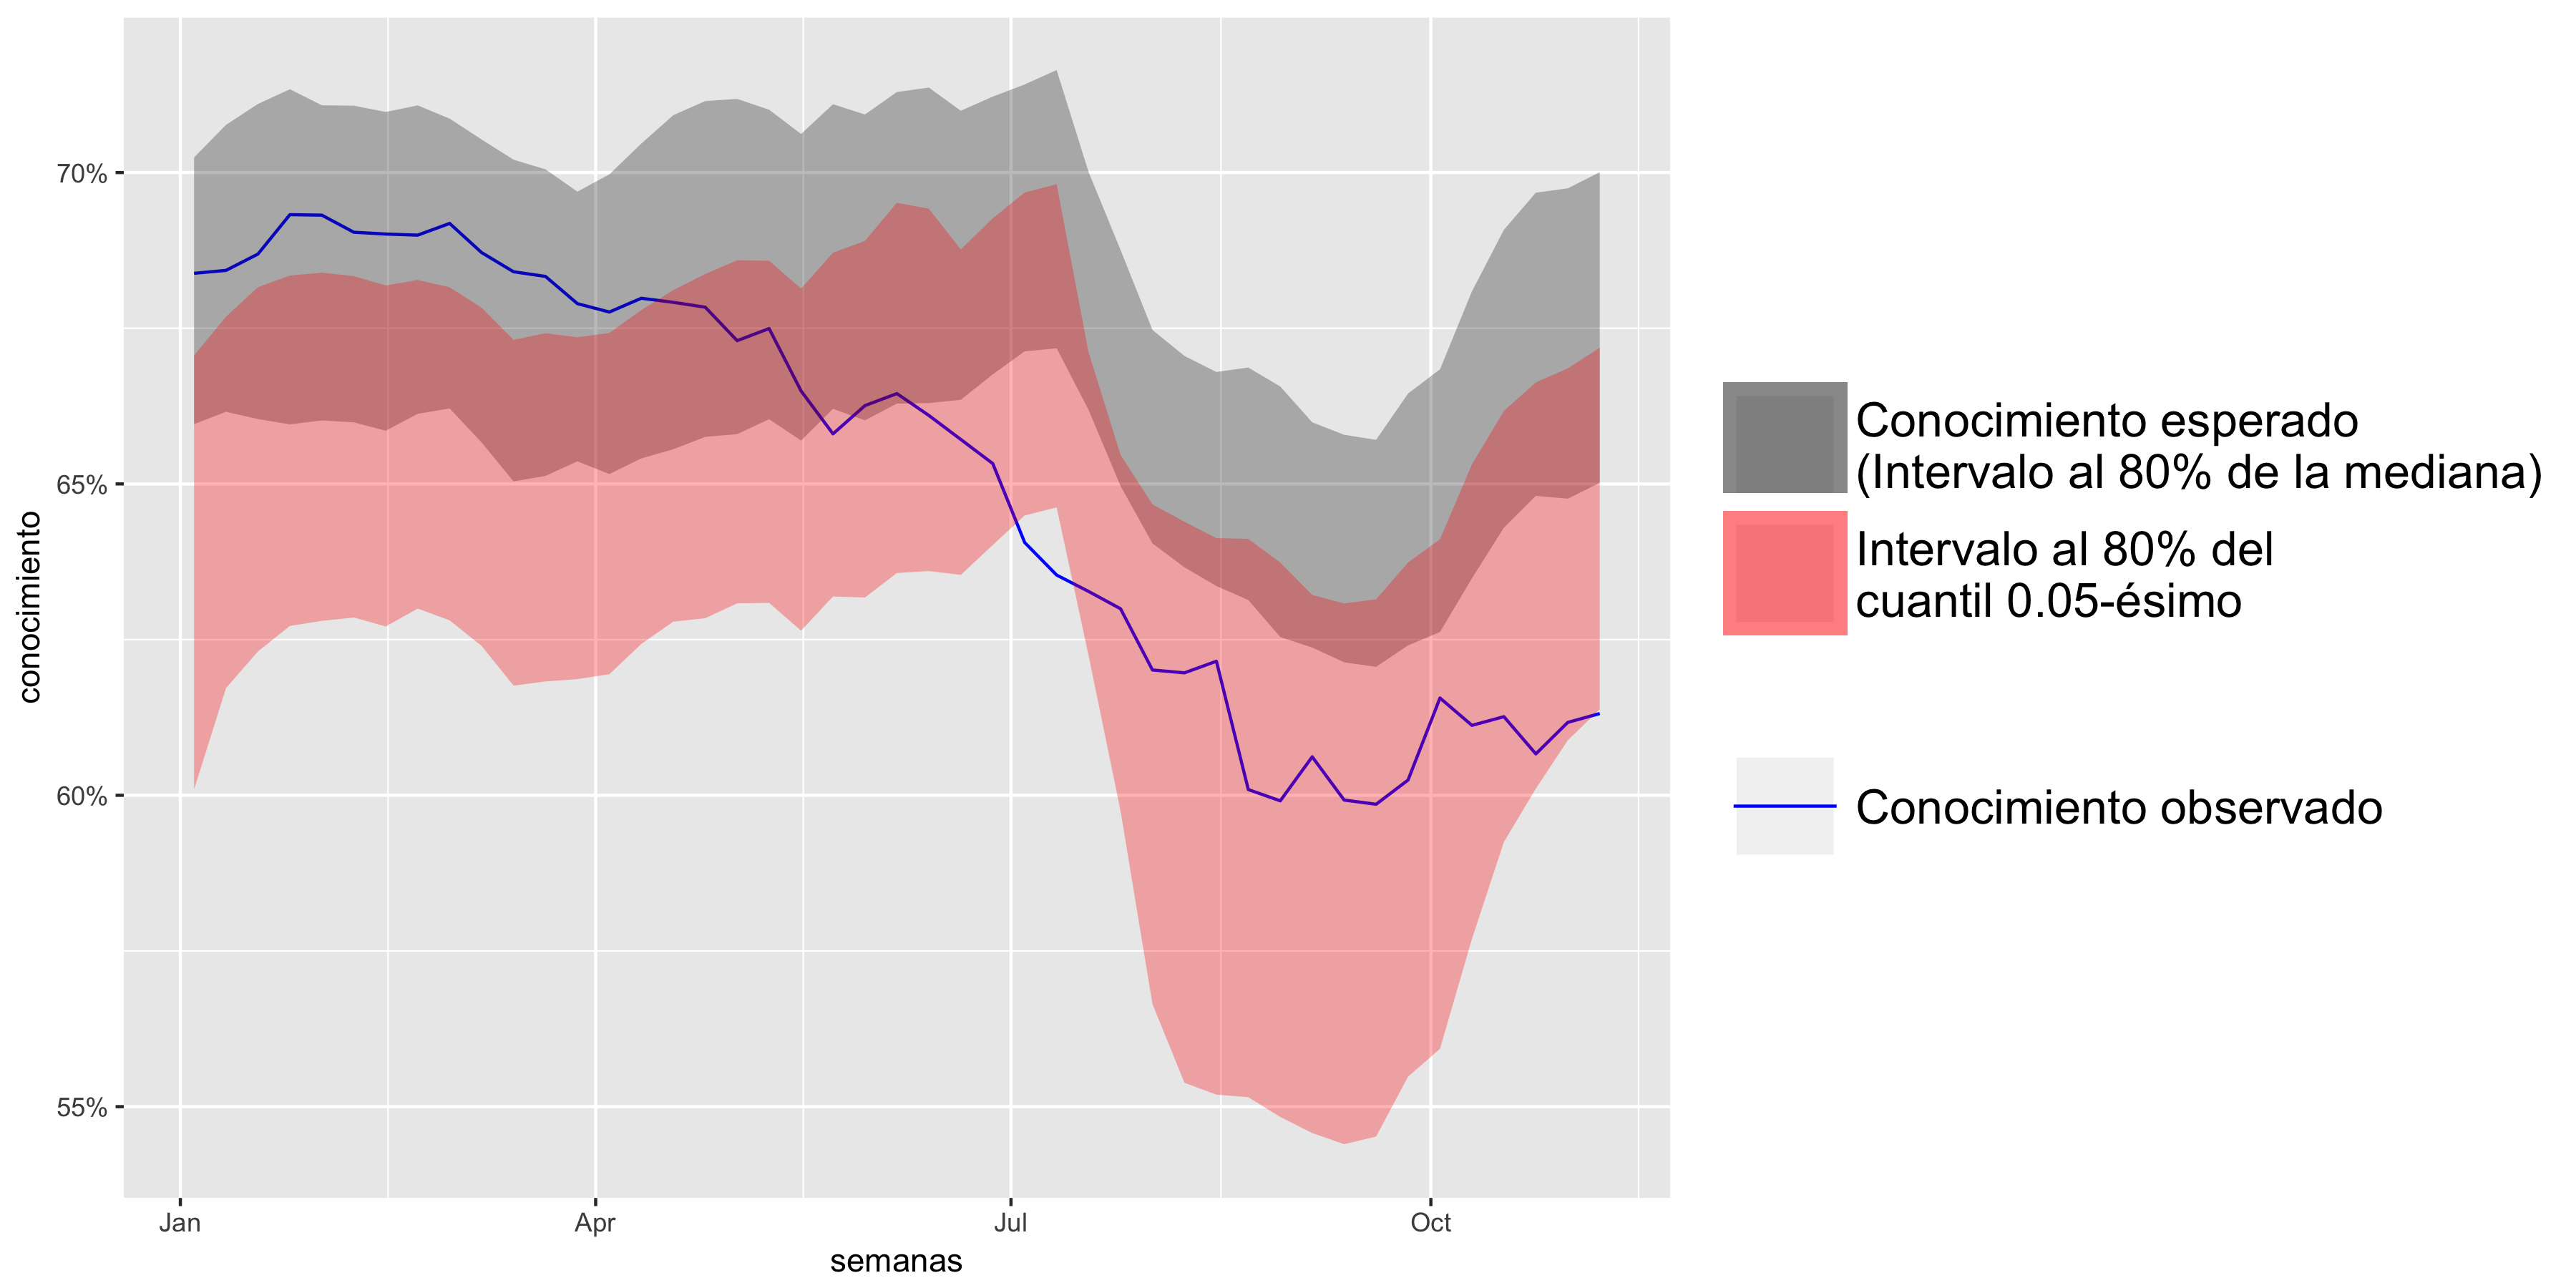
\includegraphics[width=1\textwidth]{Figures/MarketResearch/goals_2016.png}
	\captionsetup{singlelinecheck=off,font=footnotesize}
	\label{awareness_fit}
\end{figure}

Como se puede observar, hasta el mes de abril el \textit{Conocimiento de marca} se comport\'o de acuerdo a lo esperado, pero despu\'es tuvo una ca\'ida estrepitosa que, si bien el modelo hab\'ia anticipado para despu\'es de julio, coincidi\'o en mayor medida con lo que se hubiera esperado para el cuantil $0.05$-\'esimo. Es decir, suponiendo que no hubiera cambio estructural, se habr\'ia presenciado el peor de cada 20 casos.

En otras palabras, confiando en la construcci\'on del modelo, el supuesto de independencia entre las observaciones y un error modesto en la medici\'on del \textit{Conocimiento de marca}, hay informaci\'on suficiente para pensar que, en efecto, el cambio de concepto en los comerciales del competidor impact\'o la m\'etrica del cliente.


\newpage
\chapter[Conclusiones y trabajo futuro]{Conclusiones y trabajo futuro}

Si bien los modelos de regresi\'on a la media han sido de mucha utilidad en las \'ultimas d\'ecadas, principalmente cuando el poder computacional era menor, es importante darse cuenta que actualmente existen contextos en los que resultan insuficientes. Ya sea porque sea desea la mejor aproximaci\'on posible de alg\'un estad\'istico distinto a la media, o debido a que hay ocasiones en las que no se cumplen algunos de sus supuestos.

De manera similar, la relaci\'on lineal en los par\'ametros y la distribuci\'on Normal del error han sido fundamentales para que los modelos de regresi\'on hayan proliferado en una gran cantidad de industrias, tanto por su interpretabilidad, como por su bajo costo de estimaci\'on. Sin embargo, es imposible ignorar que \'unicamente representan un subconjunto del universo de funciones y errores aleatorios posibles. Crear modelos que permitan una mayor flexibilidad, como aquellos que utilizan m\'etodos no param\'etricos, lograr\'a una representaci\'on m\'as certera de la realidad de la que provienen los datos.

Al momento de hacer aproximaciones estad\'isticas, se dice que utilizar el paradigma Bayesiano muchas veces presenta la ventaja de poder introducir informaci\'on de las personas expertas en el fen\'omeno a estudiar. Desafortunadamente, en un modelo jer\'arquico, como lo es el expuesto en esta tesis, es complicado transmitir dicho conocimiento, debido a que los hiper-par\'ametros se encuentran varias capas abajo de aquellos par\'ametros que tienen una interpretaci\'on natural. A pesar de ello, vale la pena resaltar que dicha construcci\'on jer\'arquica, con la flexibilidad que brinda, es posible y es congruente gracias al paradigma Bayesiano, debido a que todas las expresiones son completamente probabil\'isticas y fundadas en un cuerpo axiom\'atico. 

Un reto importante que present\'o este trabajo fue el desarrollo del paquete en R para implementar el modelo GPDP. Primero, porque se requiri\'o plantear te\'oricamente la distribuciones condicionales necesarias para que corriera el simulador de Gibbs. Y segundo, porque tuve que buscar programar de forma general y eficiente, para que el paquete funcionara siempre que recibiera los par\'ametros predefinidos, y corriera lo m\'as r\'apido posible, ante la desventaja que representa s\'olo poder calcular una iteraci\'on de la cadena de Markov, a la vez. De hecho, dej\'e el n\'umero de iteraciones como un par\'ametro a elecci\'on del modelador, para que pueda decidir si prefiere precisi\'on o velocidad.

Si bien estos avances son significativos, a\'un existe mucho que explorar respecto a lo expuesto en esta tesis. Por ejemplo, el modelo planteado en este trabajo no es capaz de darle un peso distinto a cada variable explicativa, sino que las toma  a todas por igual al momento de calcular la distancia entre observaciones. Para mejorar esta situaci\'on se podr\'ia plantear una descomposici\'on de la funci\'on del cuantil en la suma de varios procesos Gaussianos, uno por covariable, lo que brindar\'ia un mayor peso a aquellas que en efecto sean m\'as significativas para explicar el fen\'omeno en cuesti\'on. 

Adem\'as, ser\'ia conveniente la inclusi\'on de un par\'ametro de rango que regule din\'amicamente la relaci\'on entre la distancia y la covarianza entre observaciones. Por ejemplo, a\'un cuando est\'en estandarizados los datos, una misma distancia podr\'ia significar una covarianza grande entre observaciones para alguna covariable o fen\'omeno, pero covarianza casi nula para otro. Lograr implementar este par\'ametro din\'amico seguramente mejorar\'a el ajuste.

Finalmente, tendr\'ia una gran utilidad el desarrollar una medida robusta de bondad de ajuste para este tipo de modelos. Esto brindar\'ia cualidades importantes al modelo GPDP, como el poder hacer selecci\'on de variables, y tambi\'en permitir\'ia saber qu\'e tan bueno o malo es el modelo, en comparaci\'on con lo dem\'as disponibles. 

\newpage 

%%%%%%%%%%%%%%%%%%%%%%%%%%%%%%%%%%%%%%%%%%%%%%%%%%%%%%%%%%%%%
%%    Bibliografia
%%%%%%%%%%%%%%%%%%%%%%%%%%%%%%%%%%%%%%%%%%%%%%%%%%%%%%%%%%%%%

\nocite{*} %Even non-cited BibTeX-Entries will be shown.
\bibliographystyle{authordate1}
%Style of Bibliography: plain / apalike / amsalpha / ...
\bibliography{Bibliography} 

%%%%%%%%%%%%%%%%%%%%%%%%%%%%%%%%%%%%%%%%%%%%%%%%%%%%%%%%%%%%%
%%  Apendices
%%%%%%%%%%%%%%%%%%%%%%%%%%%%%%%%%%%%%%%%%%%%%%%%%%%%%%%%%%%%%
\appendix
\chapter[Distribuciones de probabilidad]{Distribuciones de probabilidad }\label{chap:Distributions}

\section{Distribuci\'on Normal condicional}

\begin{prop*}
    Sea $X \in \mathbb{R}^m$ un vector aleatorio que tiene distribuci\'on Normal conjunta y est\'a particionado de la siguiente manera:

    \begin{equation*}
    \begin{aligned}
        X = 
        &\left[
        \begin{array}{c}
            X_1  \\
            X_2
        \end{array}
        \right], \\
        \text{ con dimensiones }
        &\left[
        \begin{array}{c}
            (m-q)  \\
            q
        \end{array}
        \right].
    \end{aligned}
    \end{equation*}
    
    Entonces, la media $\mu \in \mathbb{R}^m$ y varianza $\Sigma \in \mathbb{R}^{m \times m}$ de $X$ se pueden escribir
    \begin{equation*}
    \begin{aligned}
        \mu = 
        &\left[
        \begin{array}{c}
            \mu_1  \\
            \mu_2
        \end{array}
        \right], \\
        \text{ con dimensiones }
        &\left[
        \begin{array}{c}
            (m-q)  \\
            q
        \end{array}
        \right], y\\
        \Sigma = 
        &\left[
        \begin{array}{cc}
            \Sigma_{11} & \Sigma_{12}  \\
            \Sigma_{21} & \Sigma_{22}
        \end{array}
        \right], \\
        \text{ con dimensiones }
        &\left[
        \begin{array}{cc}
            (m-q) \times (m-q)  & (m-q) \times q  \\
            q \times (m-q) & q \times q
        \end{array}
        \right].
    \end{aligned}
    \end{equation*}
    
    La distribuci\'on condicional de $X_2$, sujeta a que $X_1 = a$ es Normal con $X_2|X_1=a \sim \mathcal{N}(X_2|\bar{\mu},\bar{\Sigma})$, donde
    
    \begin{equation*}
    \begin{aligned}
        \bar{\mu} &= \mu_2 + \Sigma_{2,1}\Sigma_{11}^{-1}(a-\mu_1) \\
        \bar{\Sigma} &= \Sigma_{22} - \Sigma_{21}\Sigma_{11}^{-1}\Sigma_{12}.
    \end{aligned}
    \end{equation*}
\end{prop*}

\section{Distribuci\'on de Dirichlet}

\begin{defin}
    Se dice que un vector aleatorio $x \in \mathbb{R}^n$ se distribuye de acuerdo a la \textbf{distribuci\'on de Dirichlet}  $\mathbf{(x \sim Dir(\alpha))}$ con vector de par\'ametros $\alpha$, espec\'ificamente,
    \begin{equation*}
        x = 
        \left(\begin{array}{c}
            x_1  \\
            \cdots \\
            x_n
        \end{array}\right),
        \qquad
        \alpha = 
        \left(\begin{array}{c}
            \alpha_1  \\
            \cdots \\
            \alpha_n
        \end{array}\right),
    \end{equation*}
    para los cuales se cumplen las restricciones
    \begin{equation*}
    \begin{aligned}
        x_i > 0, \forall i &\in \{1,...,n\} \\
        \sum_{i=1}^n x_i &= 1 \\
        \alpha_i > 0, \forall i &\in \{1,...,n\},
    \end{aligned}
    \end{equation*}
    si su funci\'on de densidad  es
    \begin{equation*}
        f(x|\alpha) = 
        \frac {1}{\mathrm {B} (\alpha)}
        \prod _{i=1}^{n}x_{i}^{\alpha _{i}-1},
    \end{equation*}
    donde $\mathrm{B}$ es la funci\'on Beta multivariada, y puede ser expresada en t\'erminos de la funci\'on $\Gamma$ como 
    \begin{equation*}
       \mathrm{B}(\alpha)=
       \frac {\prod _{i=1}^{n}\Gamma (\alpha _{i})}
       {\Gamma \left(\sum _{i=1}^{n}\alpha _{i}\right)},
       \qquad 
       \alpha =(\alpha _1,\cdots ,\alpha _n). 
    \end{equation*}
    
    La esperanza y varianza de cada $x_i$ son los siguientes:
    
    \begin{equation*}
    \begin{aligned}
        \mathbb{E}[x_i] &= \frac{\alpha_i}{\sum_{k=1}^n \alpha_k} \\
        Var(x_i) &= \frac
        {\alpha_i \left( \sum_{k=1}^n \alpha_k - \alpha_i \right)}
        {\left( \sum_{k=1}^n \alpha_k \right)^2 \left( \sum_{k=1}^n \alpha_k + 1 \right)}
    \end{aligned}
    \end{equation*}
    
\end{defin}

Es com\'un que esta distribuci\'on sea usada como la inicial conjugada de la distribuci\'on multinomial, debido a que el vector $x$ tiene las mismas propiedades de una distribuci\'on de probabilidad discreta (elementos positivos y que en conjunto suman 1).
\chapter[Algoritmos MCMC]{Algoritmos MCMC\footnote{Las ideas de este ap\'endice son retomadas de \cite{Robert_MCMC}} }\label{chap:MCMC}

\section {Introducci\'on}

Los algoritmos MCMC son utilizados para aproximar distribuciones de probabilidad, normalmente complejas. La idea es lograr simular una muestra de la distribuci\'on, para poder aproximar sus caracter\'isticas. Entre m\'as grande sea la muestra, mejor ser\'a la estimaci\'on.

Para hacer esto simula cadenas de markov de los distintos elementos de la distribuci\'on compleja, y, bajo el supuesto de que se alcanza la distribuci\'on estacionaria, toma al conjunto de dichas esas simulaciones como una muestra de la distribuci\'on original. De hecho, el nombre MCMC viene del ingl\'es \textit{Monte Carlo Markov Chains}, haciendo tambi\'en referencia a la simulaci\'on de Monte Carlo para cada iteraci\'on.

\section{Simulador de Gibbs}

Se trata de un caso particular de los algoritmos \textit{MCMC}, y a continuaci\'on se analizan dos tipos, siendo el segundo una generalizaci\'on del primero.

\subsection{Simulador de Gibbs de dos pasos}

Funciona de la siguiente manera: si dos variables aleatorias $X$ y $Y$ tienen una densidad conjunta $f(x,y)$, con sus correspondientes densidades condicionales $f_{Y|X}$ y $f_{X|Y}$, se genera una cadena de markov $(X_t,Y_t)$ de acuerdo al siguiente algoritmo:
\\ \\
\begin{algorithm}[H]
 {Tomar $X_0 = x_0$ arbitraria \;
     \For{$t=1,2,...,n$}
     {
        $1. \text{ } Y_t \sim f_{Y|X}(y|x_{t-1})\;$\\
        $2. \text{ } X_t \sim f_{X|Y}(x|y_{t})\;$
     }
 }
 \caption{Simulador de Gibbs de dos pasos}
\end{algorithm}
\BlankLine

La convergencia de la cadena de markov está asegurada, a menos que los soportes de las condicionales no estén conectados.

\subsection{Simulador de Gibbs de múltiples pasos}

Sea $\mathbb{X} \in \mathcal{X}$ una variable aleatoria que puede ser escrita como $\mathbb{X} = (X_1,...,X_p)$, con $p \in \mathbb{Z}^+$, y donde las $X_i$'s bien pueden ser unidimensionales o multidimensionales. Además, es posible encontrar las distribuciones condicionales, de forma que
\begin{equation*}
\begin{aligned}
X_i|x_1,...,x_{i-1},x_{i+1},...,x_p &\sim f_i(x_i|x_1,...,x_{i-1},x_{i+1},...,x_p) \text{, }\\
i &\in \{1,...,p\}.
\end{aligned}
\end{equation*}

El correspondiente algoritmo de Gibbs está dado por:
\\ \\
\begin{algorithm}[H]
 Tomar $\textbf{x}^{(0)} = (x_1^{(0)},...,x_p^{(0)})$ arbitraria\;
 \For{$t=1,2,...,n$}
 {
    $1. \text{ } X_1^{(t)} \sim f_1(x_1|x_2^{(t-1)},...,x_p^{(t-1)})\;$\\
    $2. \text{ } X_2^{(t)} \sim f_2(x_2|x_1^{(t)},x_3^{(t-1)},...,x_p^{(t-1)})\;$\\
    $...\;$\\
    $k.  \text{ } X_k^{(t)} \sim f_k(x_k|x_1^{(t)},...,x_{k-1}^{(t)},x_{k+1}^{(t-1)},...,x_p^{(t-1)})\;$\\
    $...\;$\\
    $p.  \text{ }X_p^{(t)} \sim f_p(x_p|x_1^{(t)},...,x_{p-1}^{(t)})\;$\\
 }
 \caption{Simulador de Gibbs de múltiples pasos}
\end{algorithm}
\BlankLine

Cabe resaltar que el desempeño puede estar fuertemente afectado por la parametrización del modelo. Por ello puede resultar una buena idea reparametrizar el modelo, buscando que las componentes sean lo más independientes posible.

\section {Monitoreo de convergencia y adaptación de los algortimos MCMC}

\subsection{Monitoreo de convergencia a la \textit{estacionariedad}}

El primer requisito de convergencia de un algoritmo MCMC es que la distribución de la cadena $(x^{(t)})$ sea la distribución estacionaria $f$. Una meta menos ambiciosa sería que sea independiente del punto inicial $x^{(0)}$, después de muchas realizaciones de la cadena. La principal herramienta para verificar \textit{estacionariedad} es correr varias cadenas en paralelo, para poder comparar sus rendimientos. 

Un primer acercamiento empírico al control de convergencia es el dibujar gráficas de las cadenas simuladas (componente a componente o juntas), para detectar valores muy desviados y comportamientos no estacionarios. 

Otro diagnóstico gráfico que se puede utilizar es la \textit{traza}, es decir, la gr\'afica de cada uno de los valores de la cadena en el eje $y$, contra su respectivo n\'umero de iteraci\'on en el eje $x$. As\'i ser\'a posible observar cuando la cadena tiene un comportamiento repetitivo en ciertos valores y a partir de qu\'e momento se distribuye sobre todo el soporte, es decir, a partir de qu\'e iteraci\'on alcanza la distribuci\'on estacionaria. 

\subsection{Monitoreo de convergencia a los promedios}

Una vez cubierta la distribución estacionaria, se verifica la convergencia del promedio aritmético
\begin{equation*}
    \frac{1}{T}\sum_{t=1}^T h(x^{(t)})
\end{equation*}
a la esperanza $\mathbb{E}_f[h(x)]$, para una función $h$ arbitraria. Esto propiedad se denomina com\'unmente \textit{ergodicidad}.

La herramienta inicial y más natural suele ser el graficar la evolución del estimador del promedio, conforme crece $T$. Si dicha curva no se ha estabilizado después de $T$ iteraciones, habría que incrementar la longitud de la cadena de markov.

\subsection{Monitoreo de convergencia a una muestra \textit{iid}}

Para finalizar, idealmente, la aproximación de $f$ obtenida de los algortimos MCMC se debería extender a la producción (aproximada) de muestras $iid$ de $f$. La técnica más usada para lograr esto es el \textit{submuestreo o refinamiento}, donde se consideran s\'olo los valores $y^{(t)} = x^{(kt)}$, para cierta $k$.

Como medidas diagn\'ostico normalmente se usan las siguientes: la autocorrelaci\'on dentro de cada variable aleatoria que es parte del simulador de Gibbs; y la correlaci\'on cruzada entre las distintas variables aleatorias, dado que se busca independencia entre ellas.

\newpage

\end{document}

